\setlength{\footskip}{8mm}

\chapter{PRELIMINARY RESULT}
    \section{Code Repository and Deployment}
        \subsection{GitHub Repository} 
        The GitHub repository provides all essential code, configurations, and documentation for the AIT Match project, offering a comprehensive overview of its technical setup. It includes database schemas, controller logic, feature implementations, Docker configurations, and dataset seeding files. This repository serves as a valuable resource for understanding the platform's infrastructure, design, and development processes.
        
        \begin{figure}[h]
        \centering
        
\includegraphics[width=1.2in]{figures/qr-code-github.png} 
        \captionsetup{justification=centering, singlelinecheck=false, labelsep=space}
        \caption{\href{https://github.com/werrnnnwerrrnnnnnn/AIT-Match}{GitHub Repository: AIT Match}}
        \label{fig:github_qr}
        \end{figure}

        \subsection{DockerHub Repository}
        The DockerHub repository hosts a pre-configured Docker image of the AIT Match platform, based on the source files from GitHub. This image allows quick deployment with all required dependencies and configurations, facilitating a seamless setup across various environments. The DockerHub repository streamlines deployment and ensures consistency in both development and production. Additionally, the platform is deployed on the CSIM (Computer Science \& Information Management) server at the Asian Institute of Technology (AIT), providing an institutionally supported and secure environment for the platform’s users within the university.

        \begin{figure}[h]
        \centering
        
\includegraphics[width=1.2in]{figures/qr-code-dockerhub.png} 
        \captionsetup{justification=centering, singlelinecheck=false, labelsep=space}
        \caption{\href{https://hub.docker.com/repository/docker/werrnnnwerrrnnnnnn/match_web/general}{Dockerhub Repository: AIT Match}}
        \label{fig:dockerhub_qr}
        \end{figure}

    \newpage
    \section{User Interface Results}
    
        \subsection{Landing Page: Welcome}
        \begin{figure}[h]
                \centering
                \captionsetup{justification=centering, singlelinecheck=false, labelsep=space}
                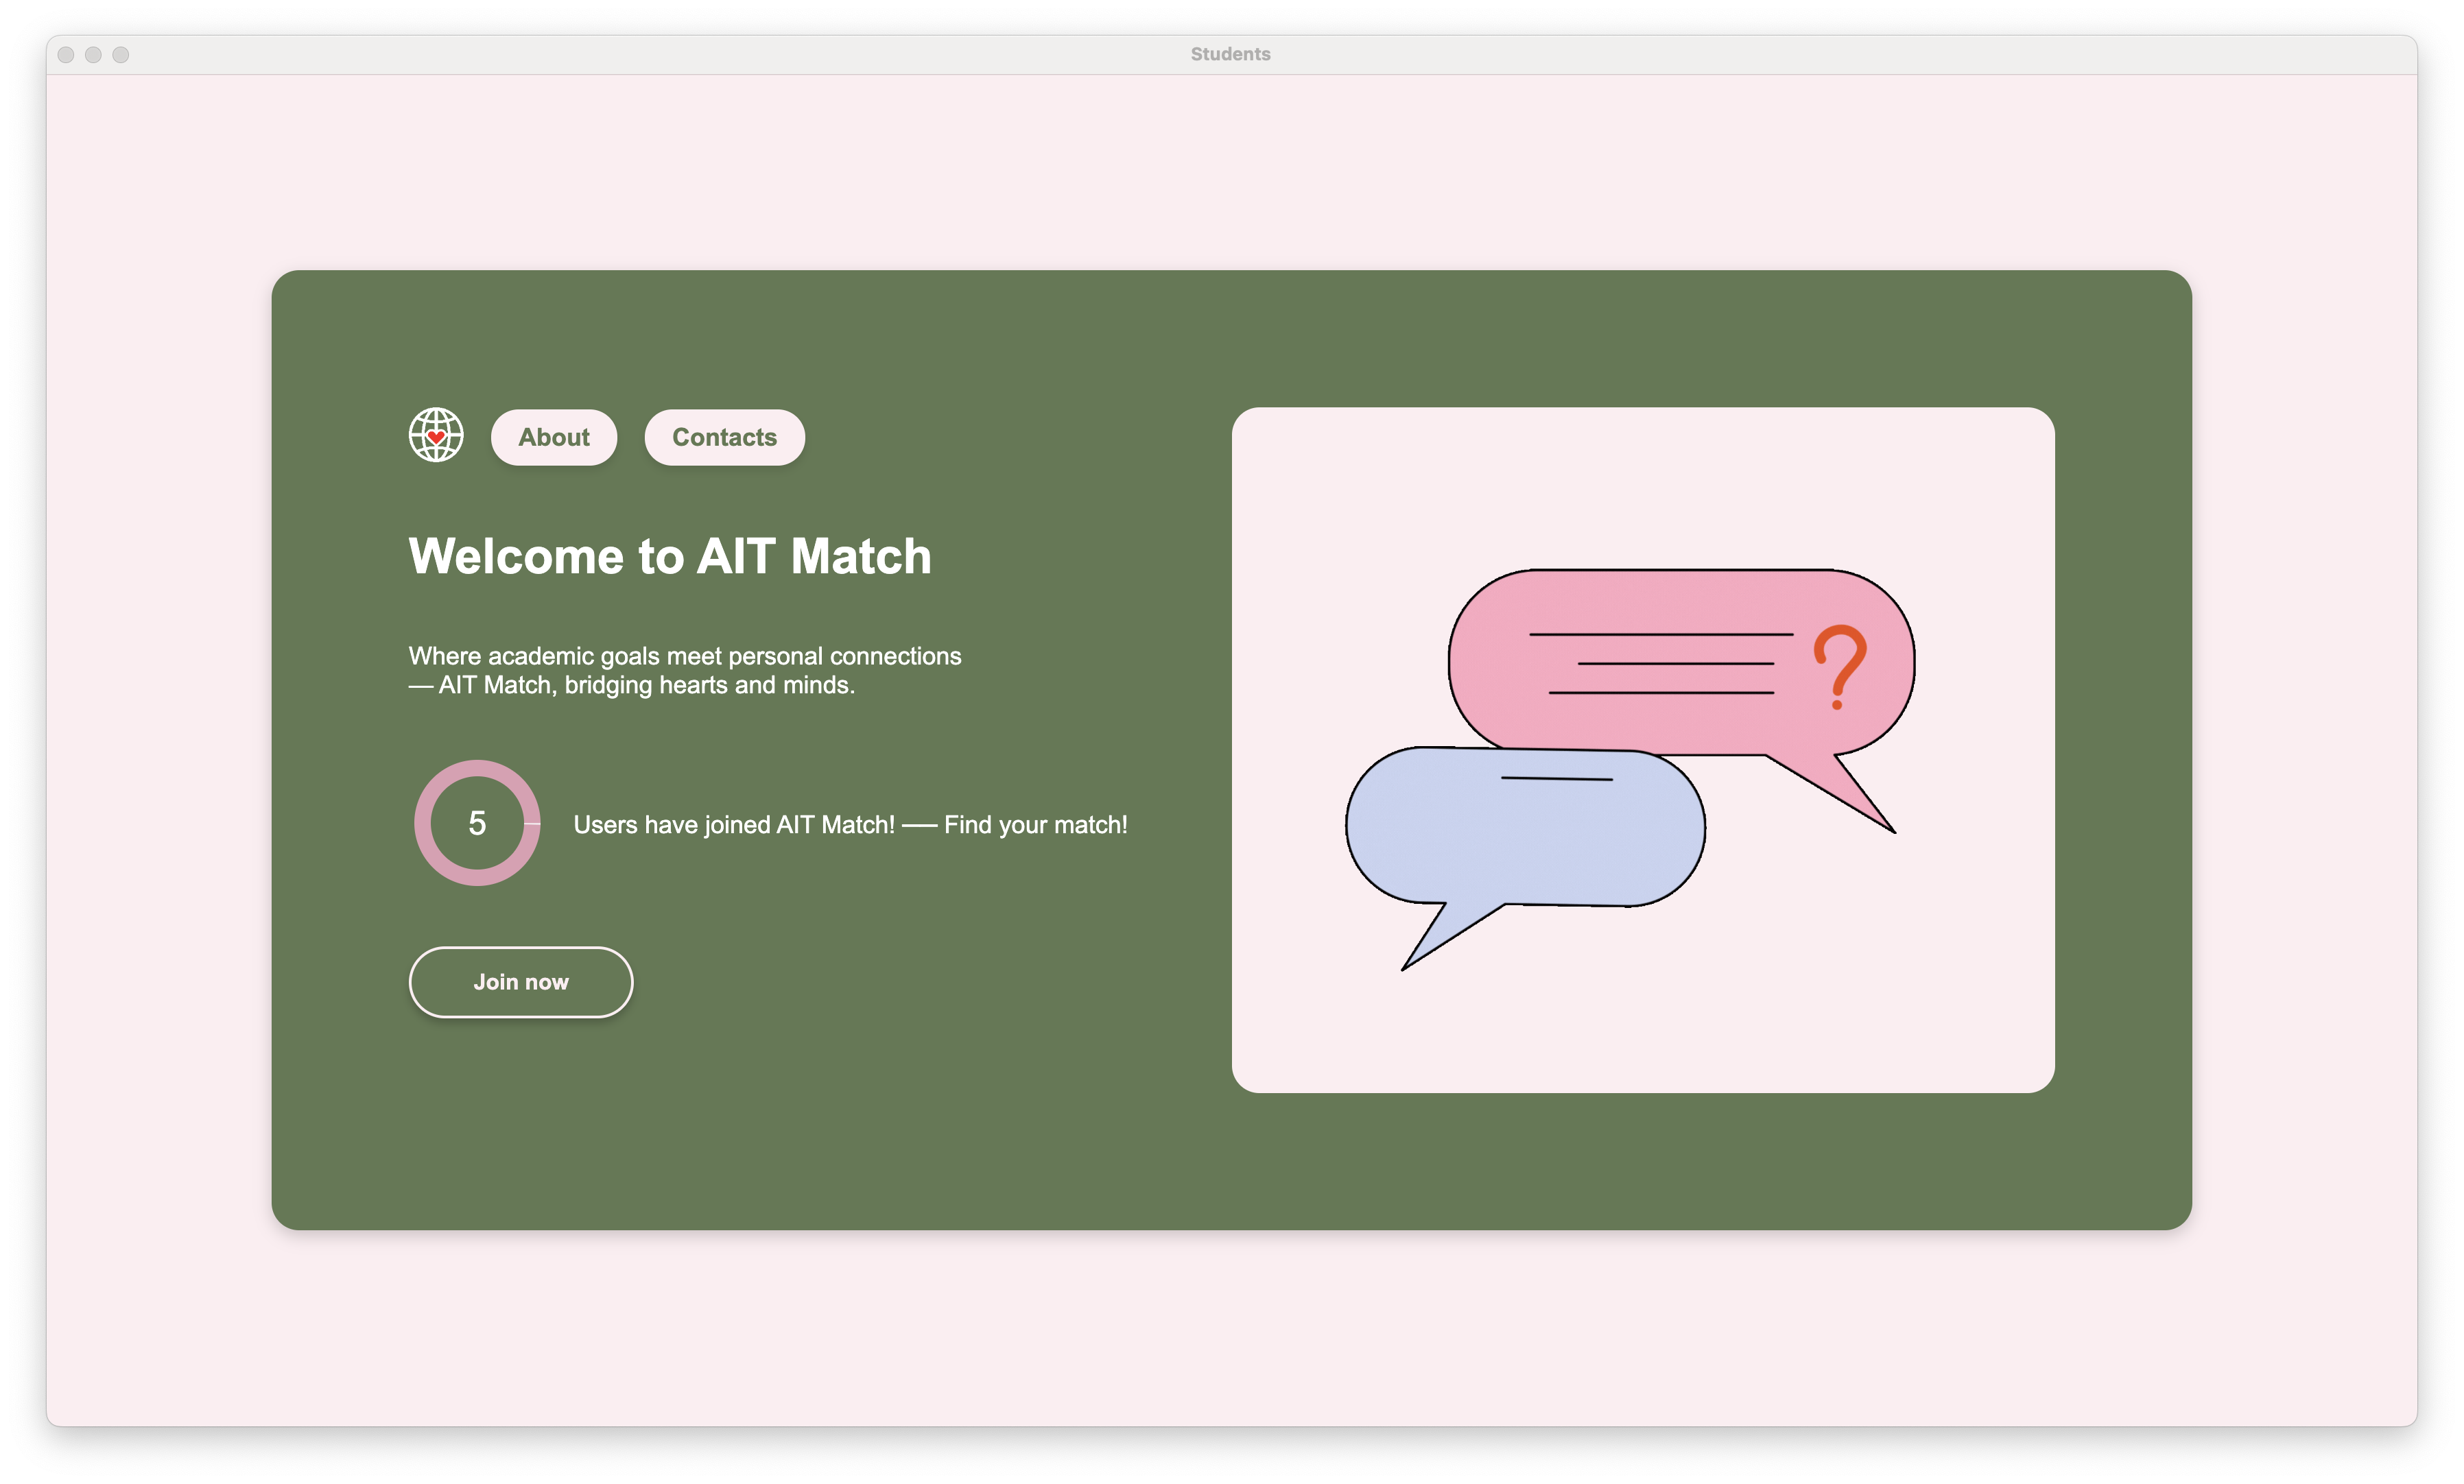
\includegraphics[width=5in]{figures/results/landing-page/welcome-page.png} 
                \caption{Welcome Page.}
                \label{fig:welcome-page}
            \end{figure}  

        \subsection{Landing Page: About}
        \begin{figure}[h]
                \centering
                \captionsetup{justification=centering, singlelinecheck=false, labelsep=space}
                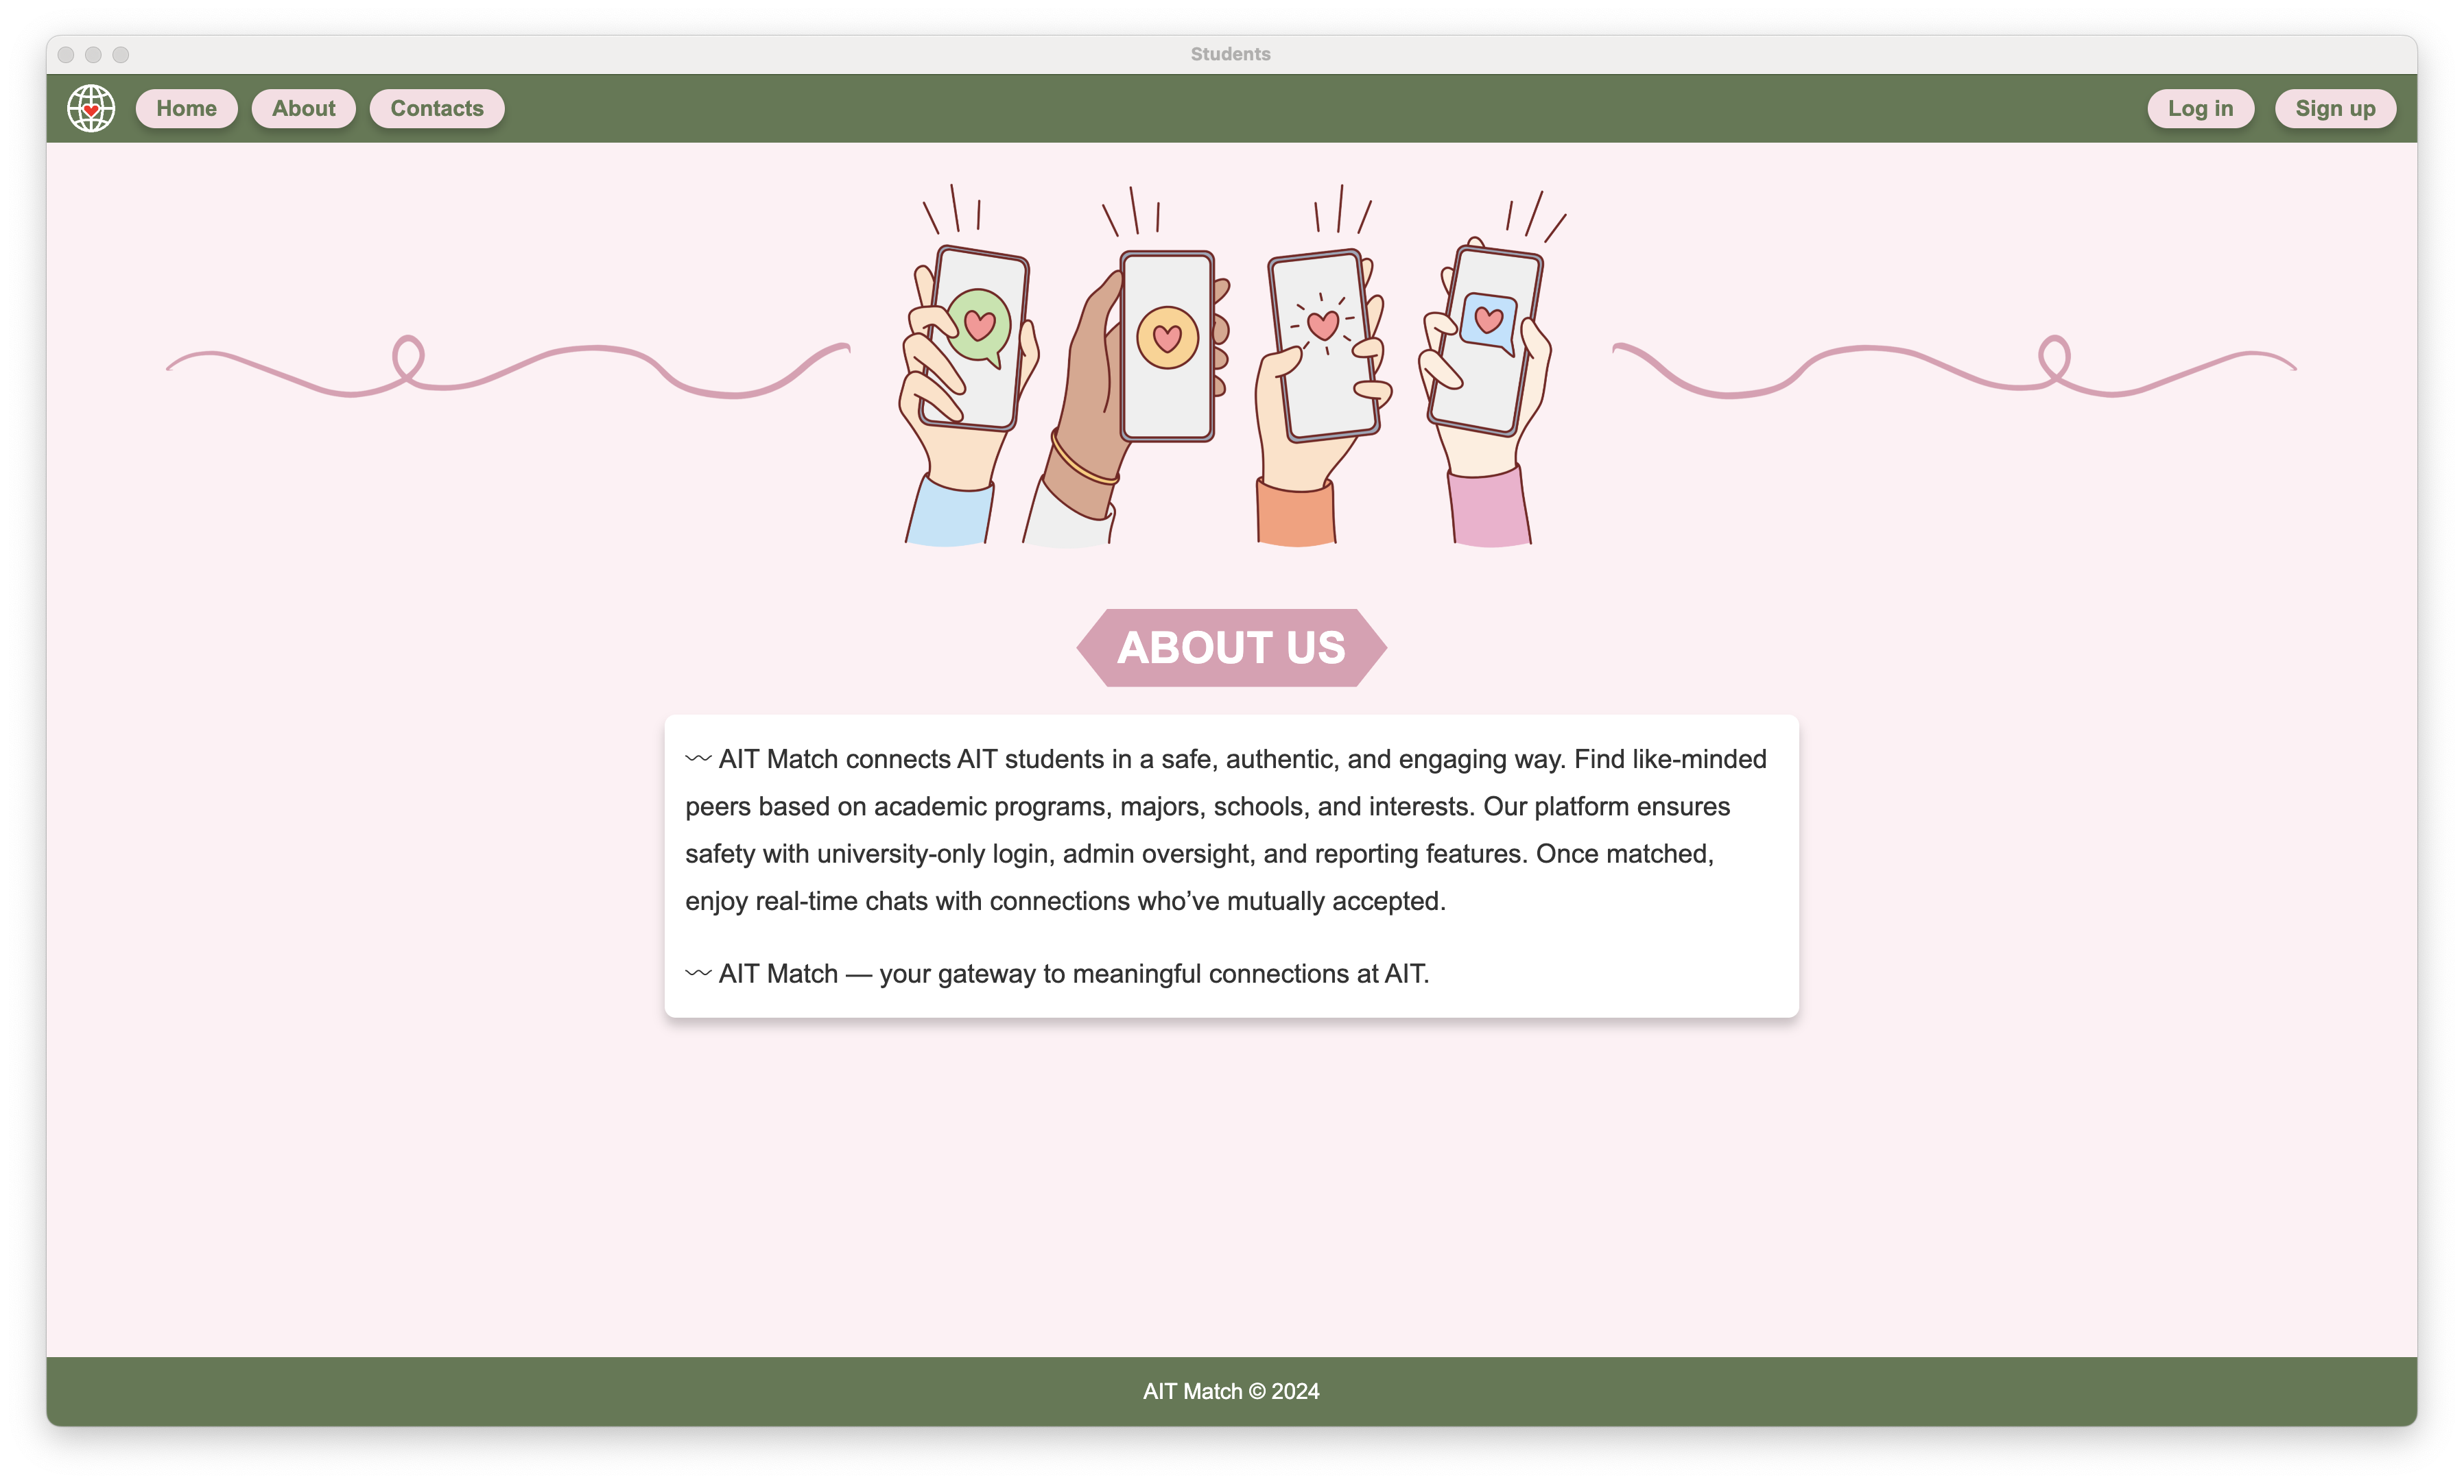
\includegraphics[width=5in]{figures/results/landing-page/about-page.png} 
                \caption{About Page.}
                \label{fig:about-page}
            \end{figure}  

        \newpage
        \subsection{Landing Page: Contact}
        \begin{figure}[h]
                \centering
                \captionsetup{justification=centering, singlelinecheck=false, labelsep=space}
                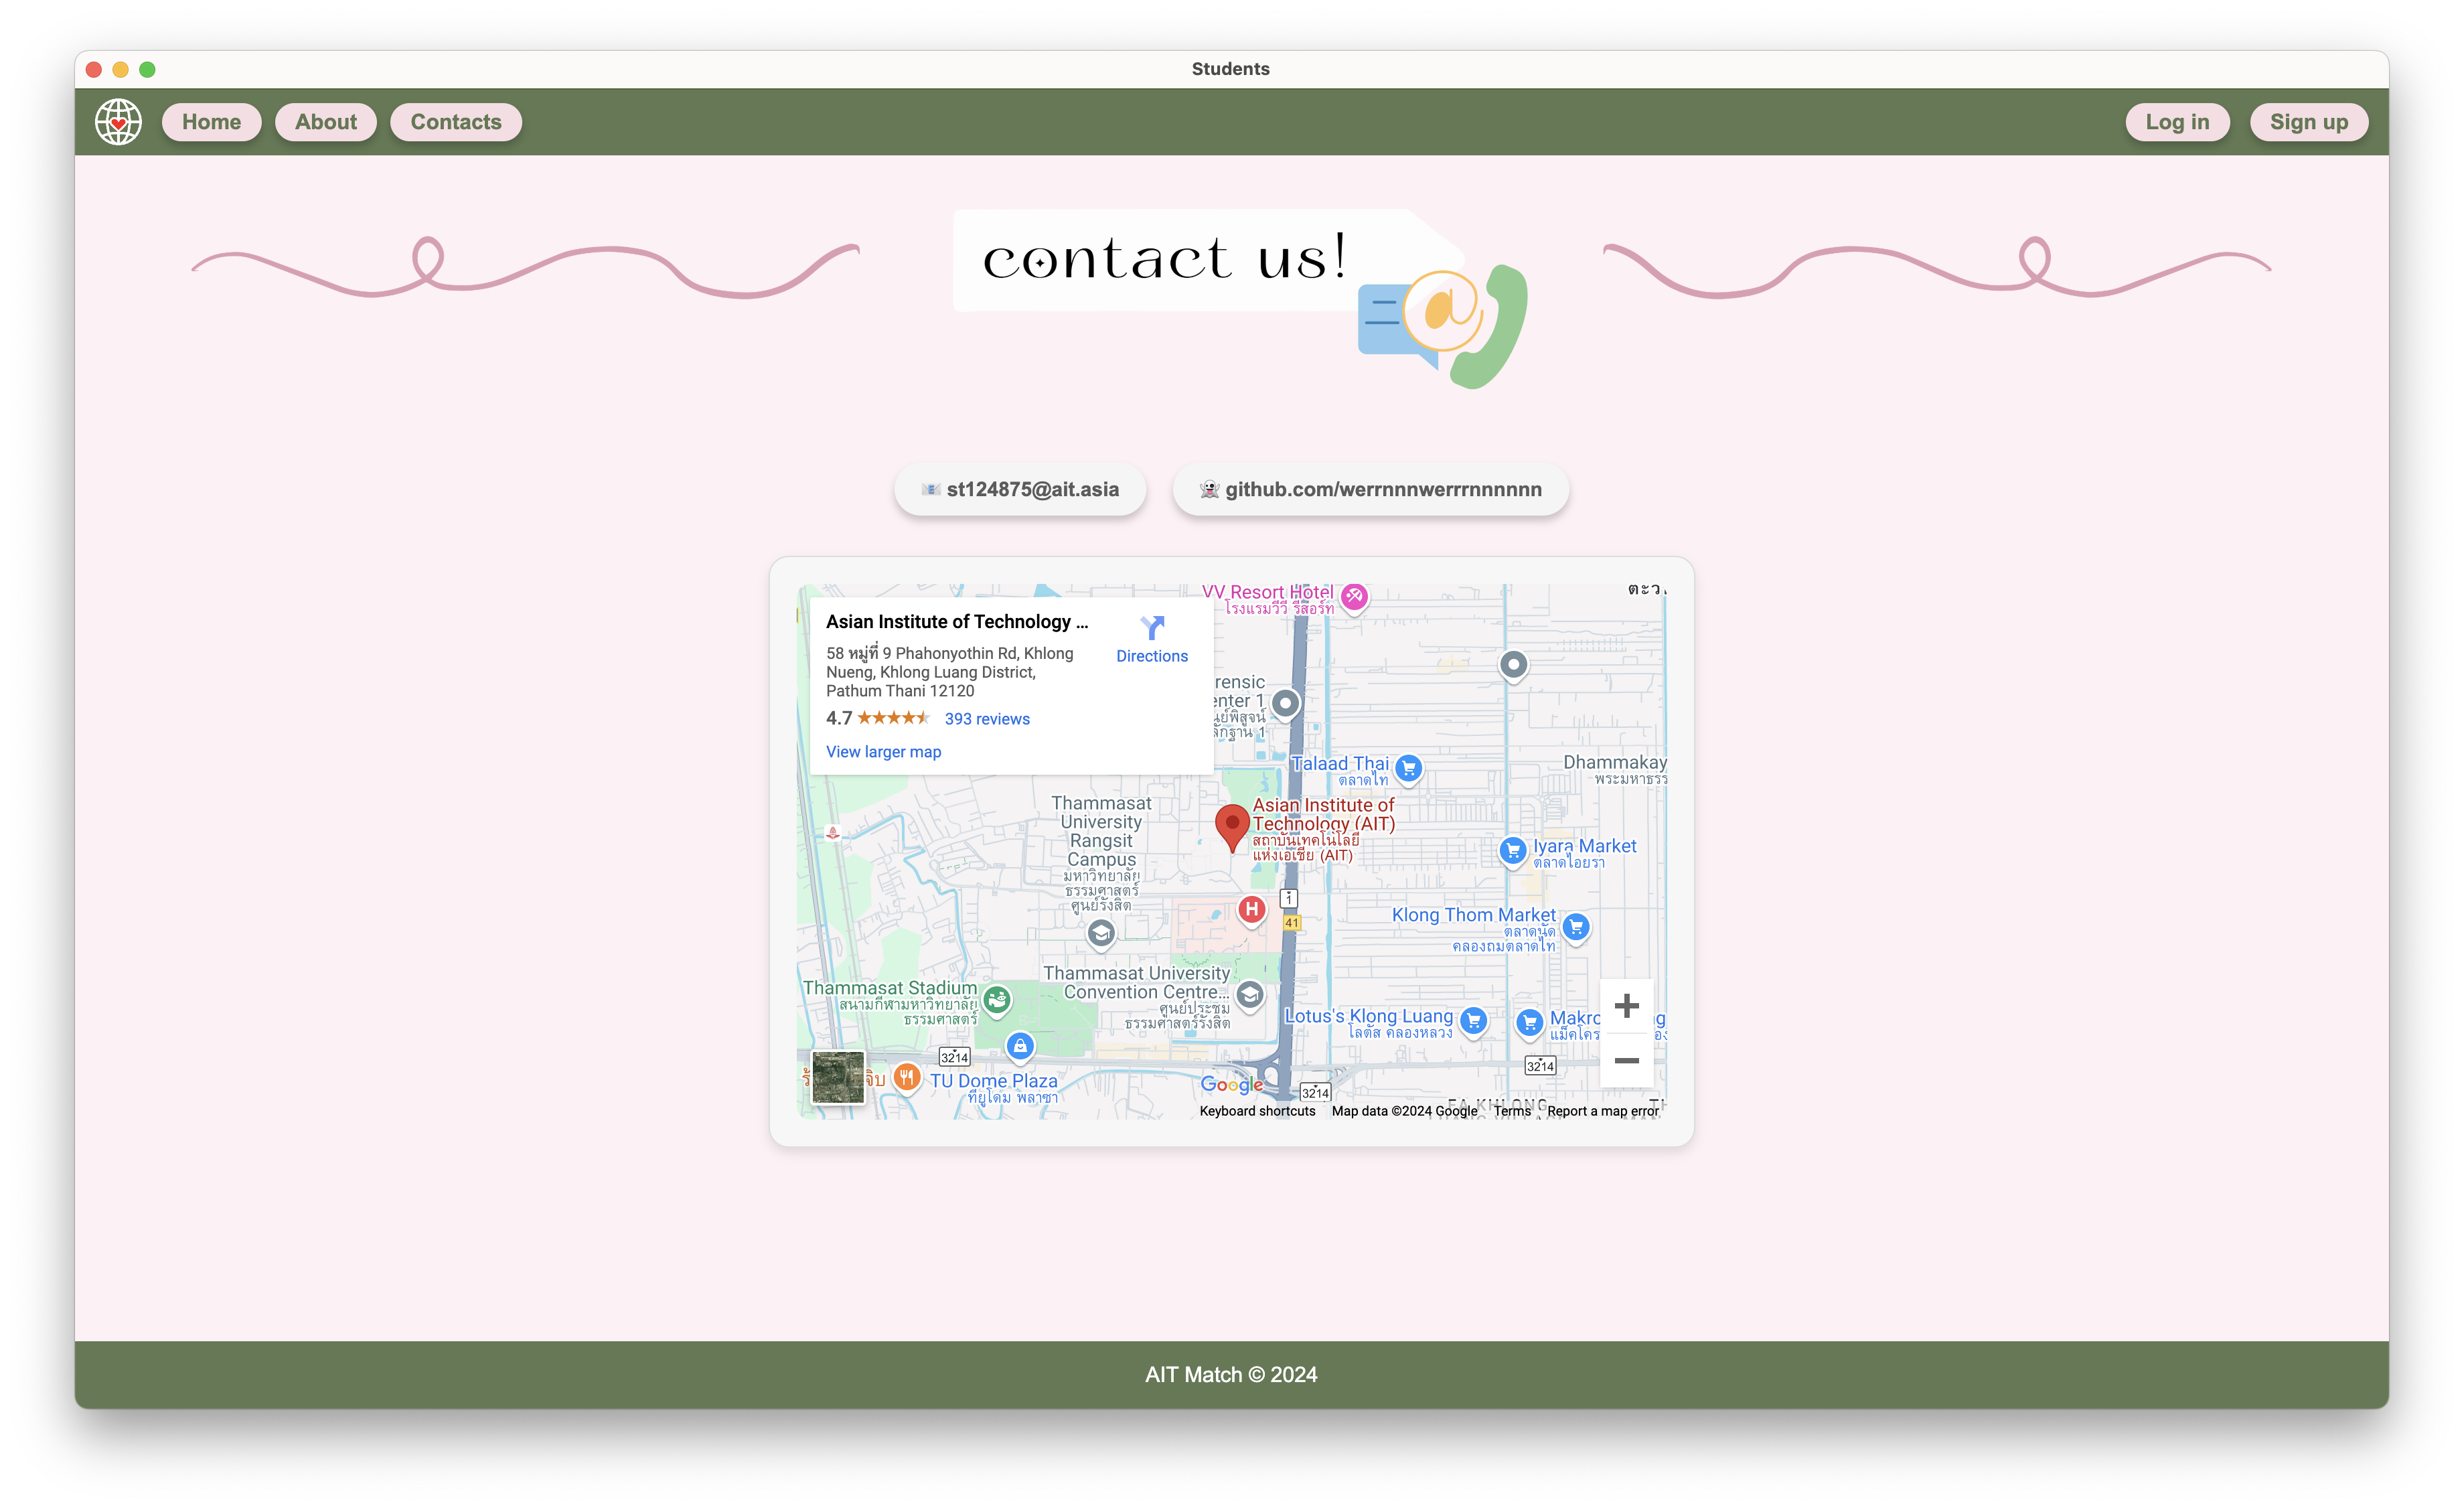
\includegraphics[width=5in]{figures/results/landing-page/contact-page.png} 
                \caption{Contact Page.}
                \label{fig:contact-page}
            \end{figure}  
% ------------------------------------------------- %
        \newpage
        \subsection{User Authentication: Sign Up Page}
        \begin{figure}[h]
                \centering
                \captionsetup{justification=centering, singlelinecheck=false, labelsep=space}
                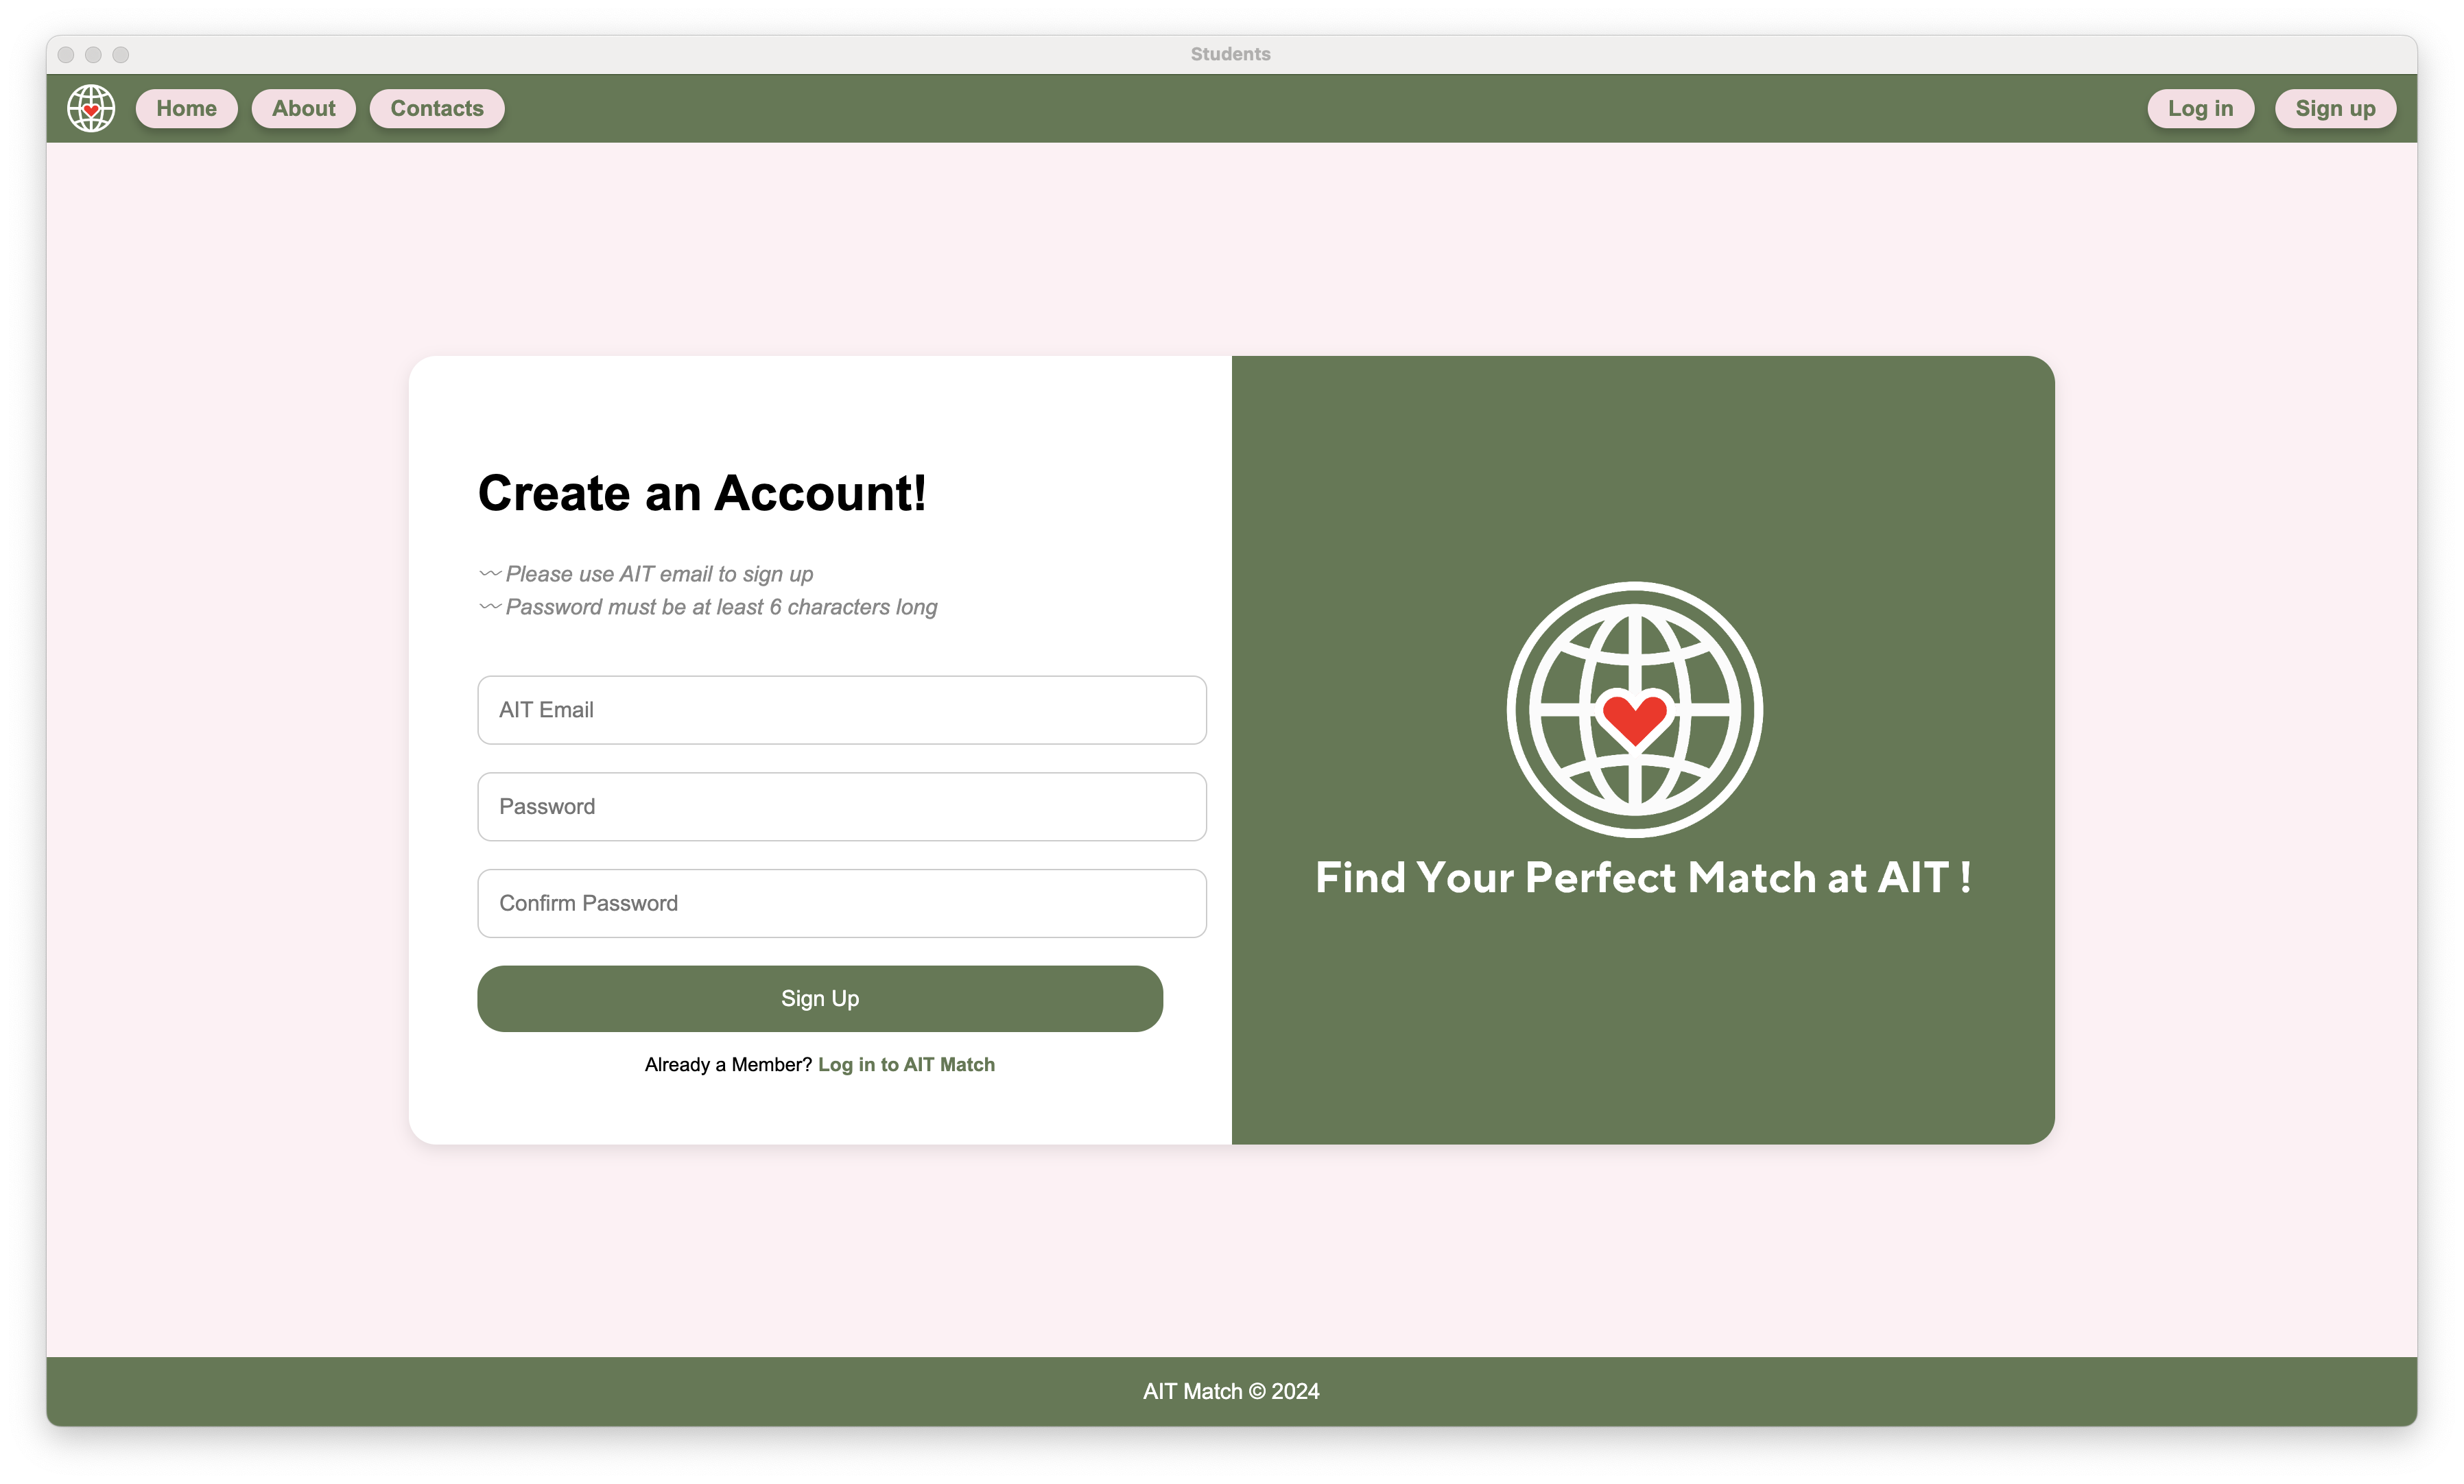
\includegraphics[width=5in]{figures/results/landing-page/signup-page.png} 
                \caption{Sign Up Page.}
                \label{fig:signup-page}
            \end{figure}

        \subsection{User Authentication Page: Login Page}
        \begin{figure}[h]
                \centering
                \captionsetup{justification=centering, singlelinecheck=false, labelsep=space}
                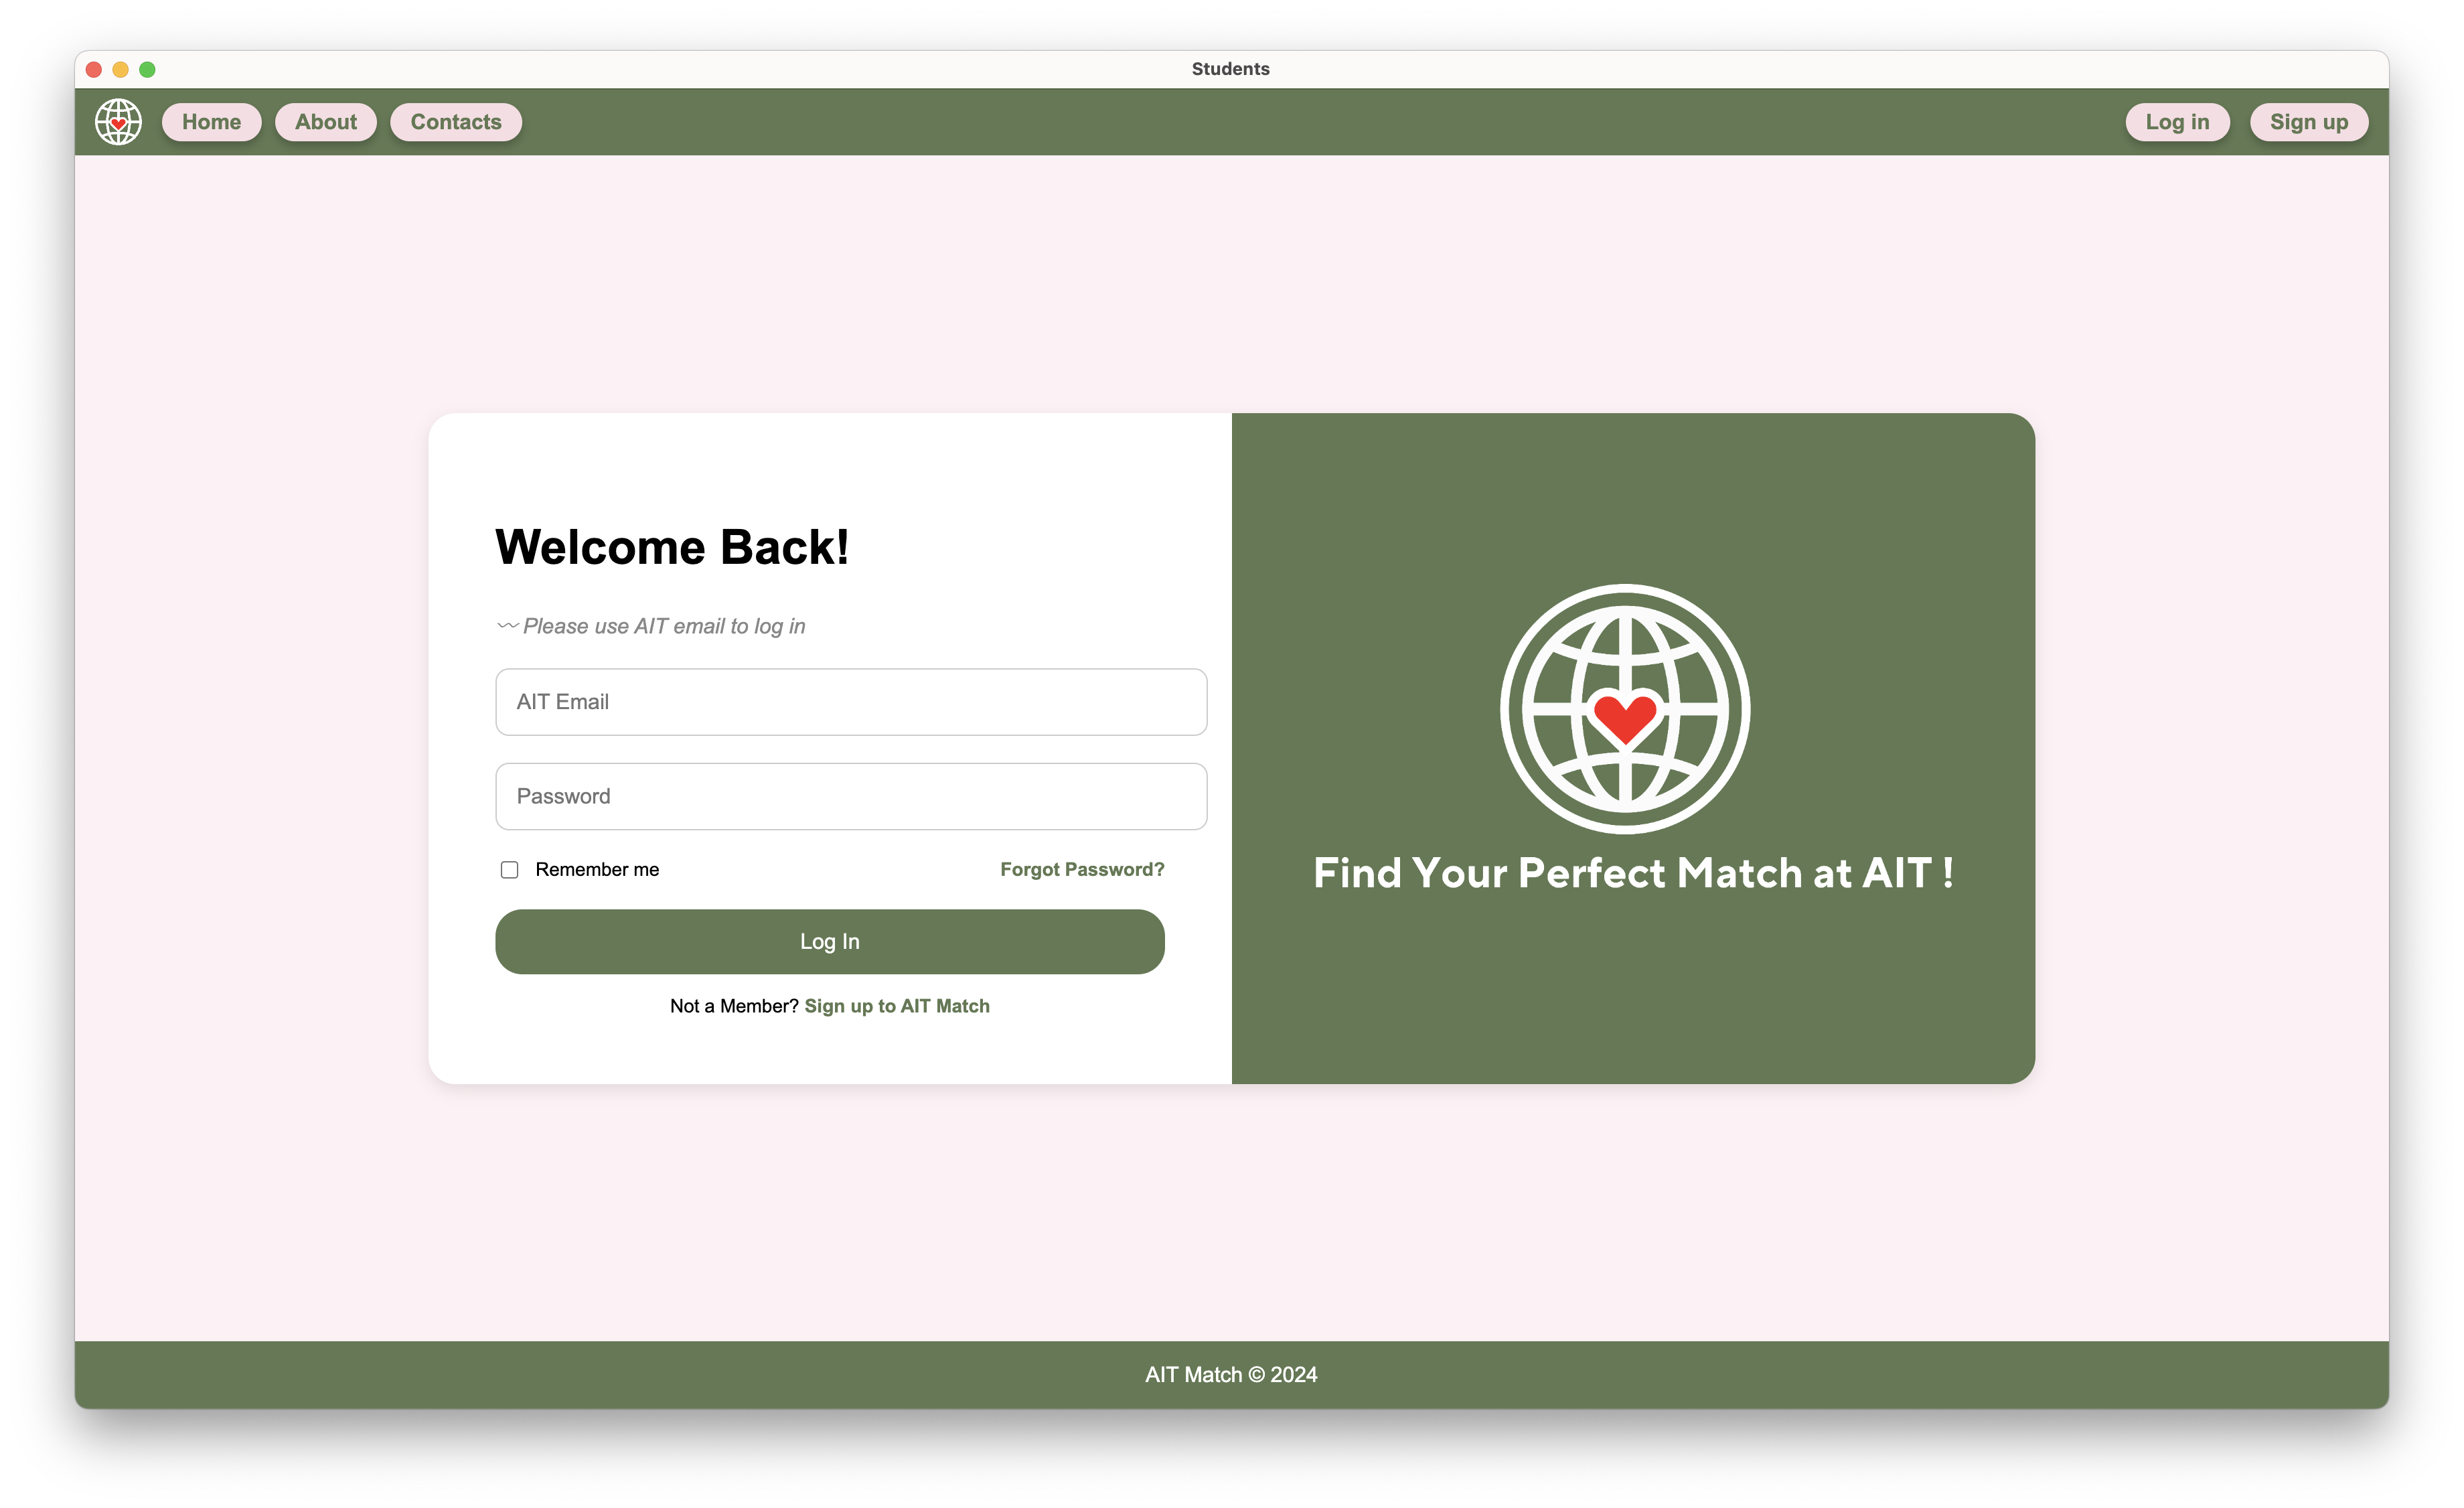
\includegraphics[width=5in]{figures/results/landing-page/login-page.png} 
                \caption{Login Page.}
                \label{fig:login-page}
            \end{figure}
% ------------------------------------------------- %
        \newpage
        \subsection{Profile: Profile Creation Page}
        \begin{figure}[h]
                \centering
                \captionsetup{justification=centering, singlelinecheck=false, labelsep=space}
                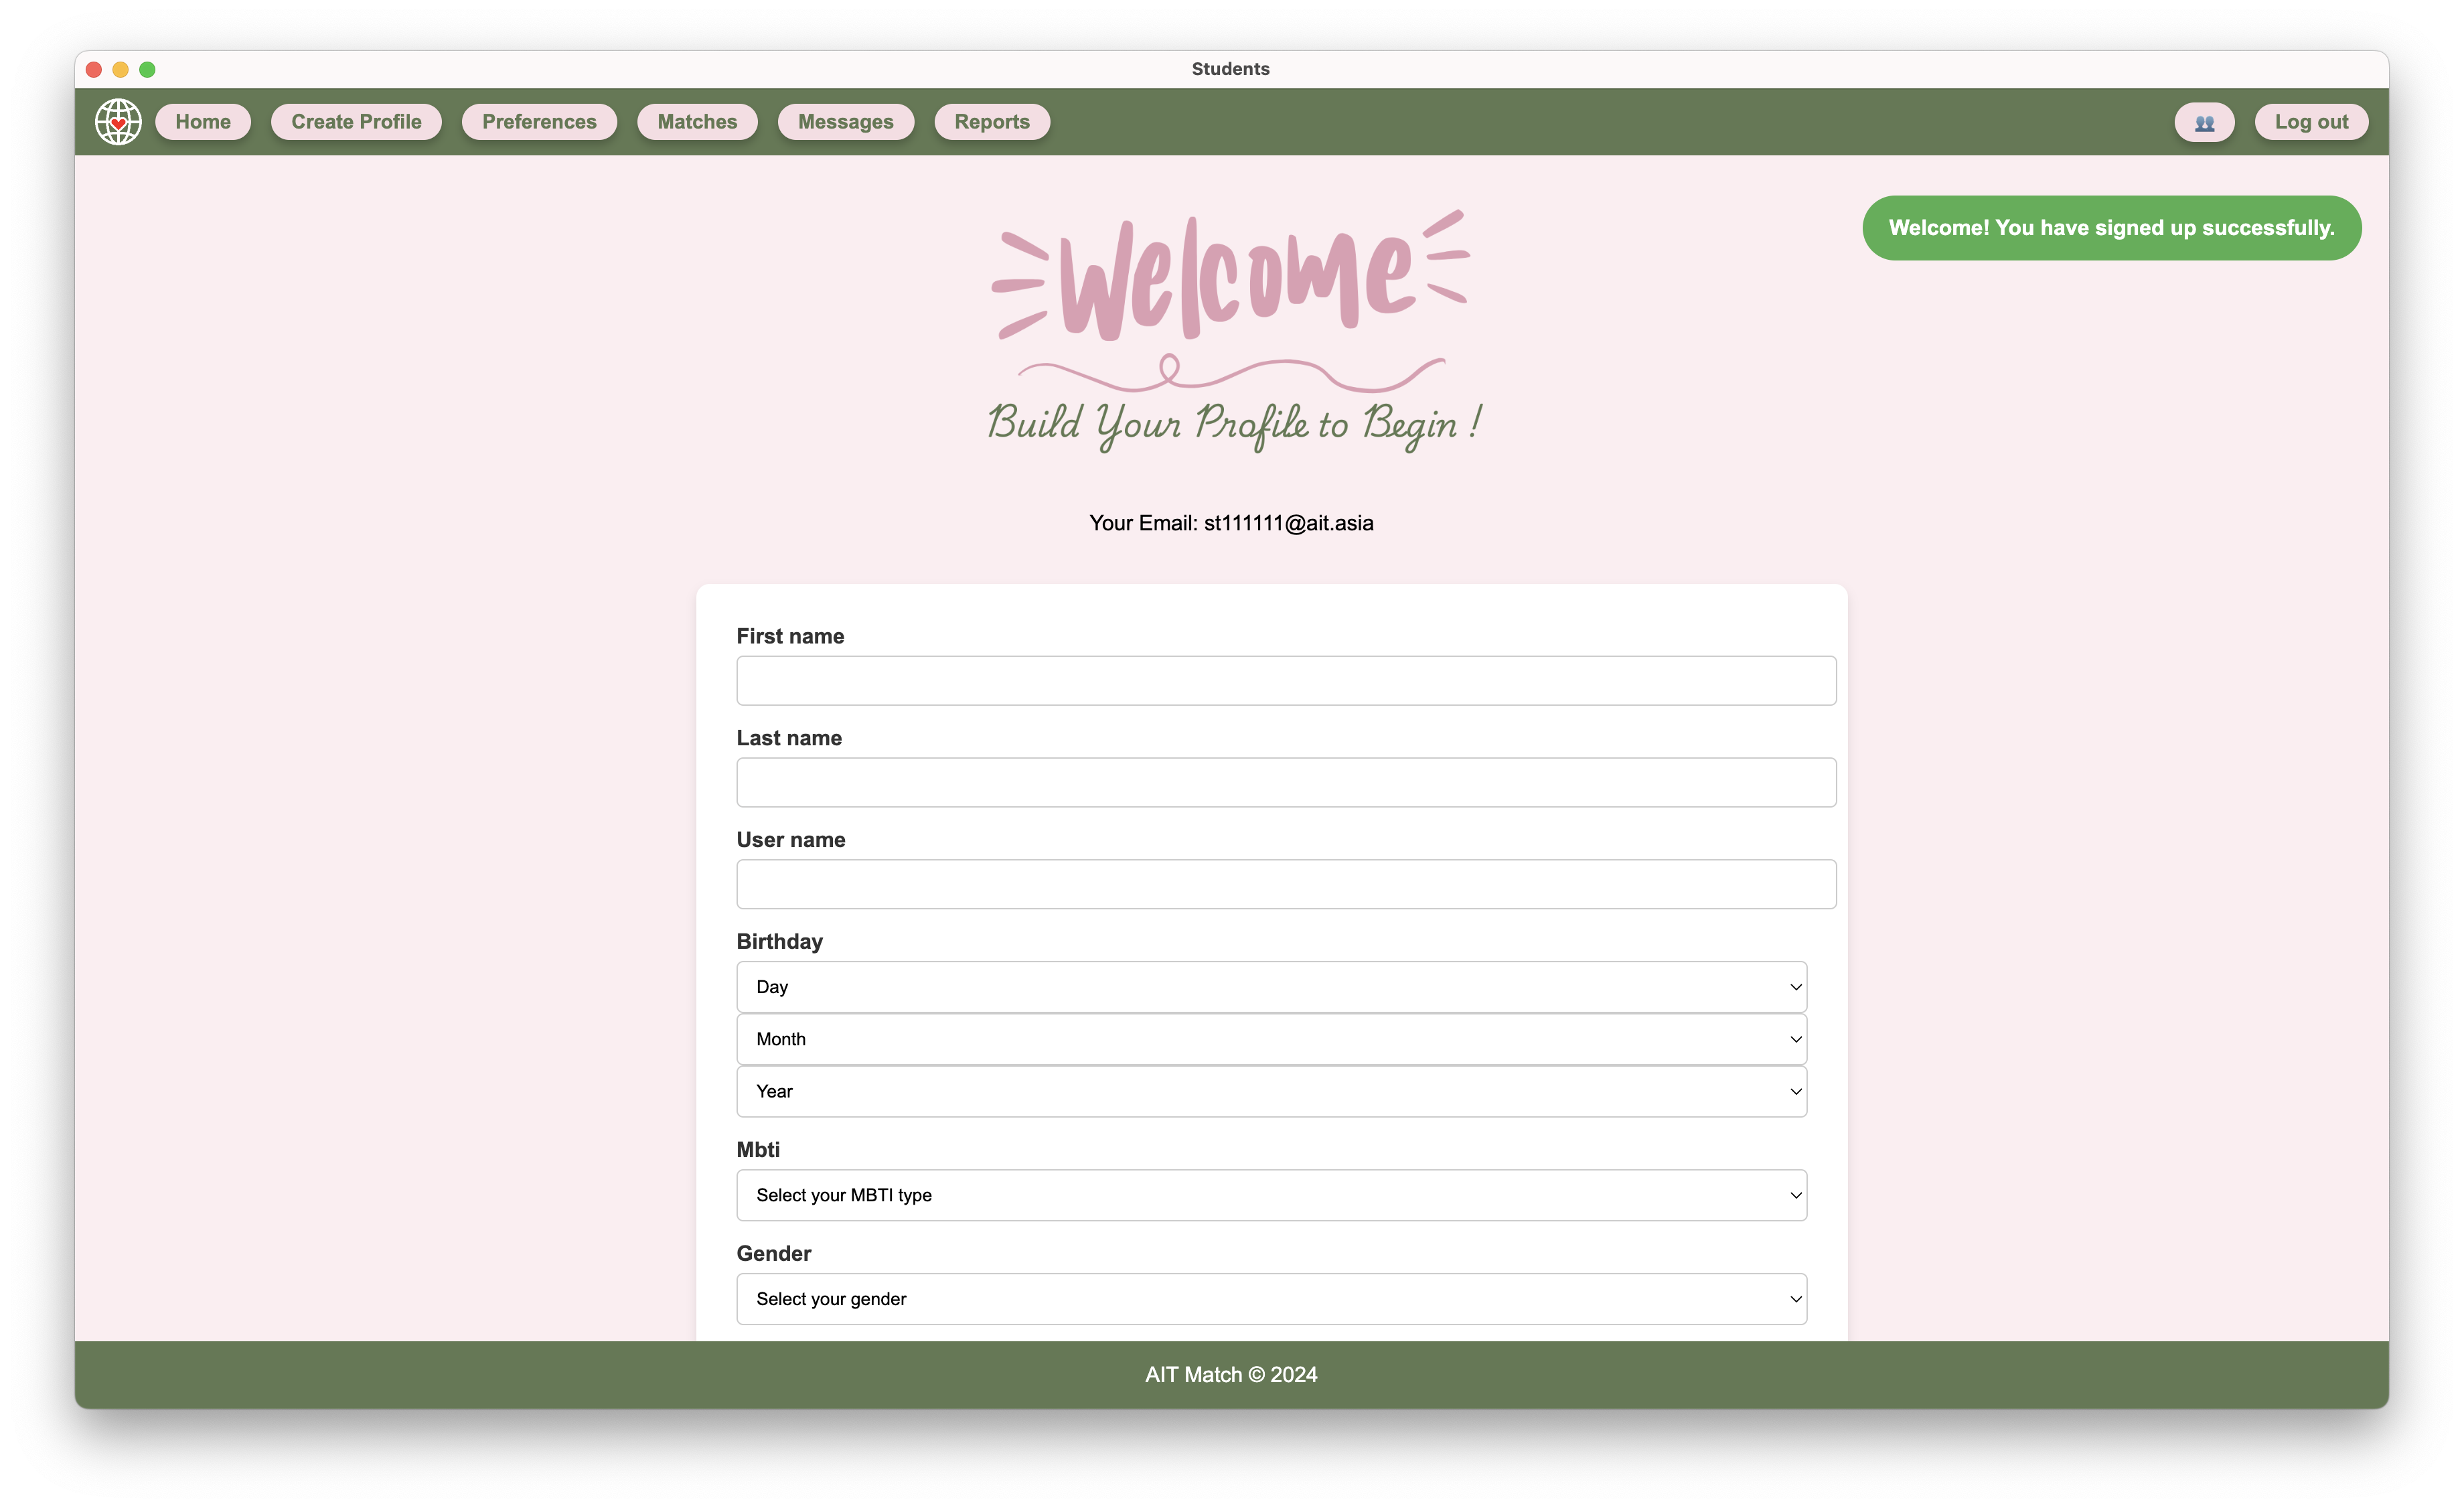
\includegraphics[width=5in]{figures/results/profiles/create-profile-page.png} 
                \caption{Profile CreationPage.}
                \label{fig:create-profile-page}
            \end{figure}

        \subsection{Profile: Profile Creation Page (Continued)}
        \begin{figure}[h]
                \centering
                \captionsetup{justification=centering, singlelinecheck=false, labelsep=space}
                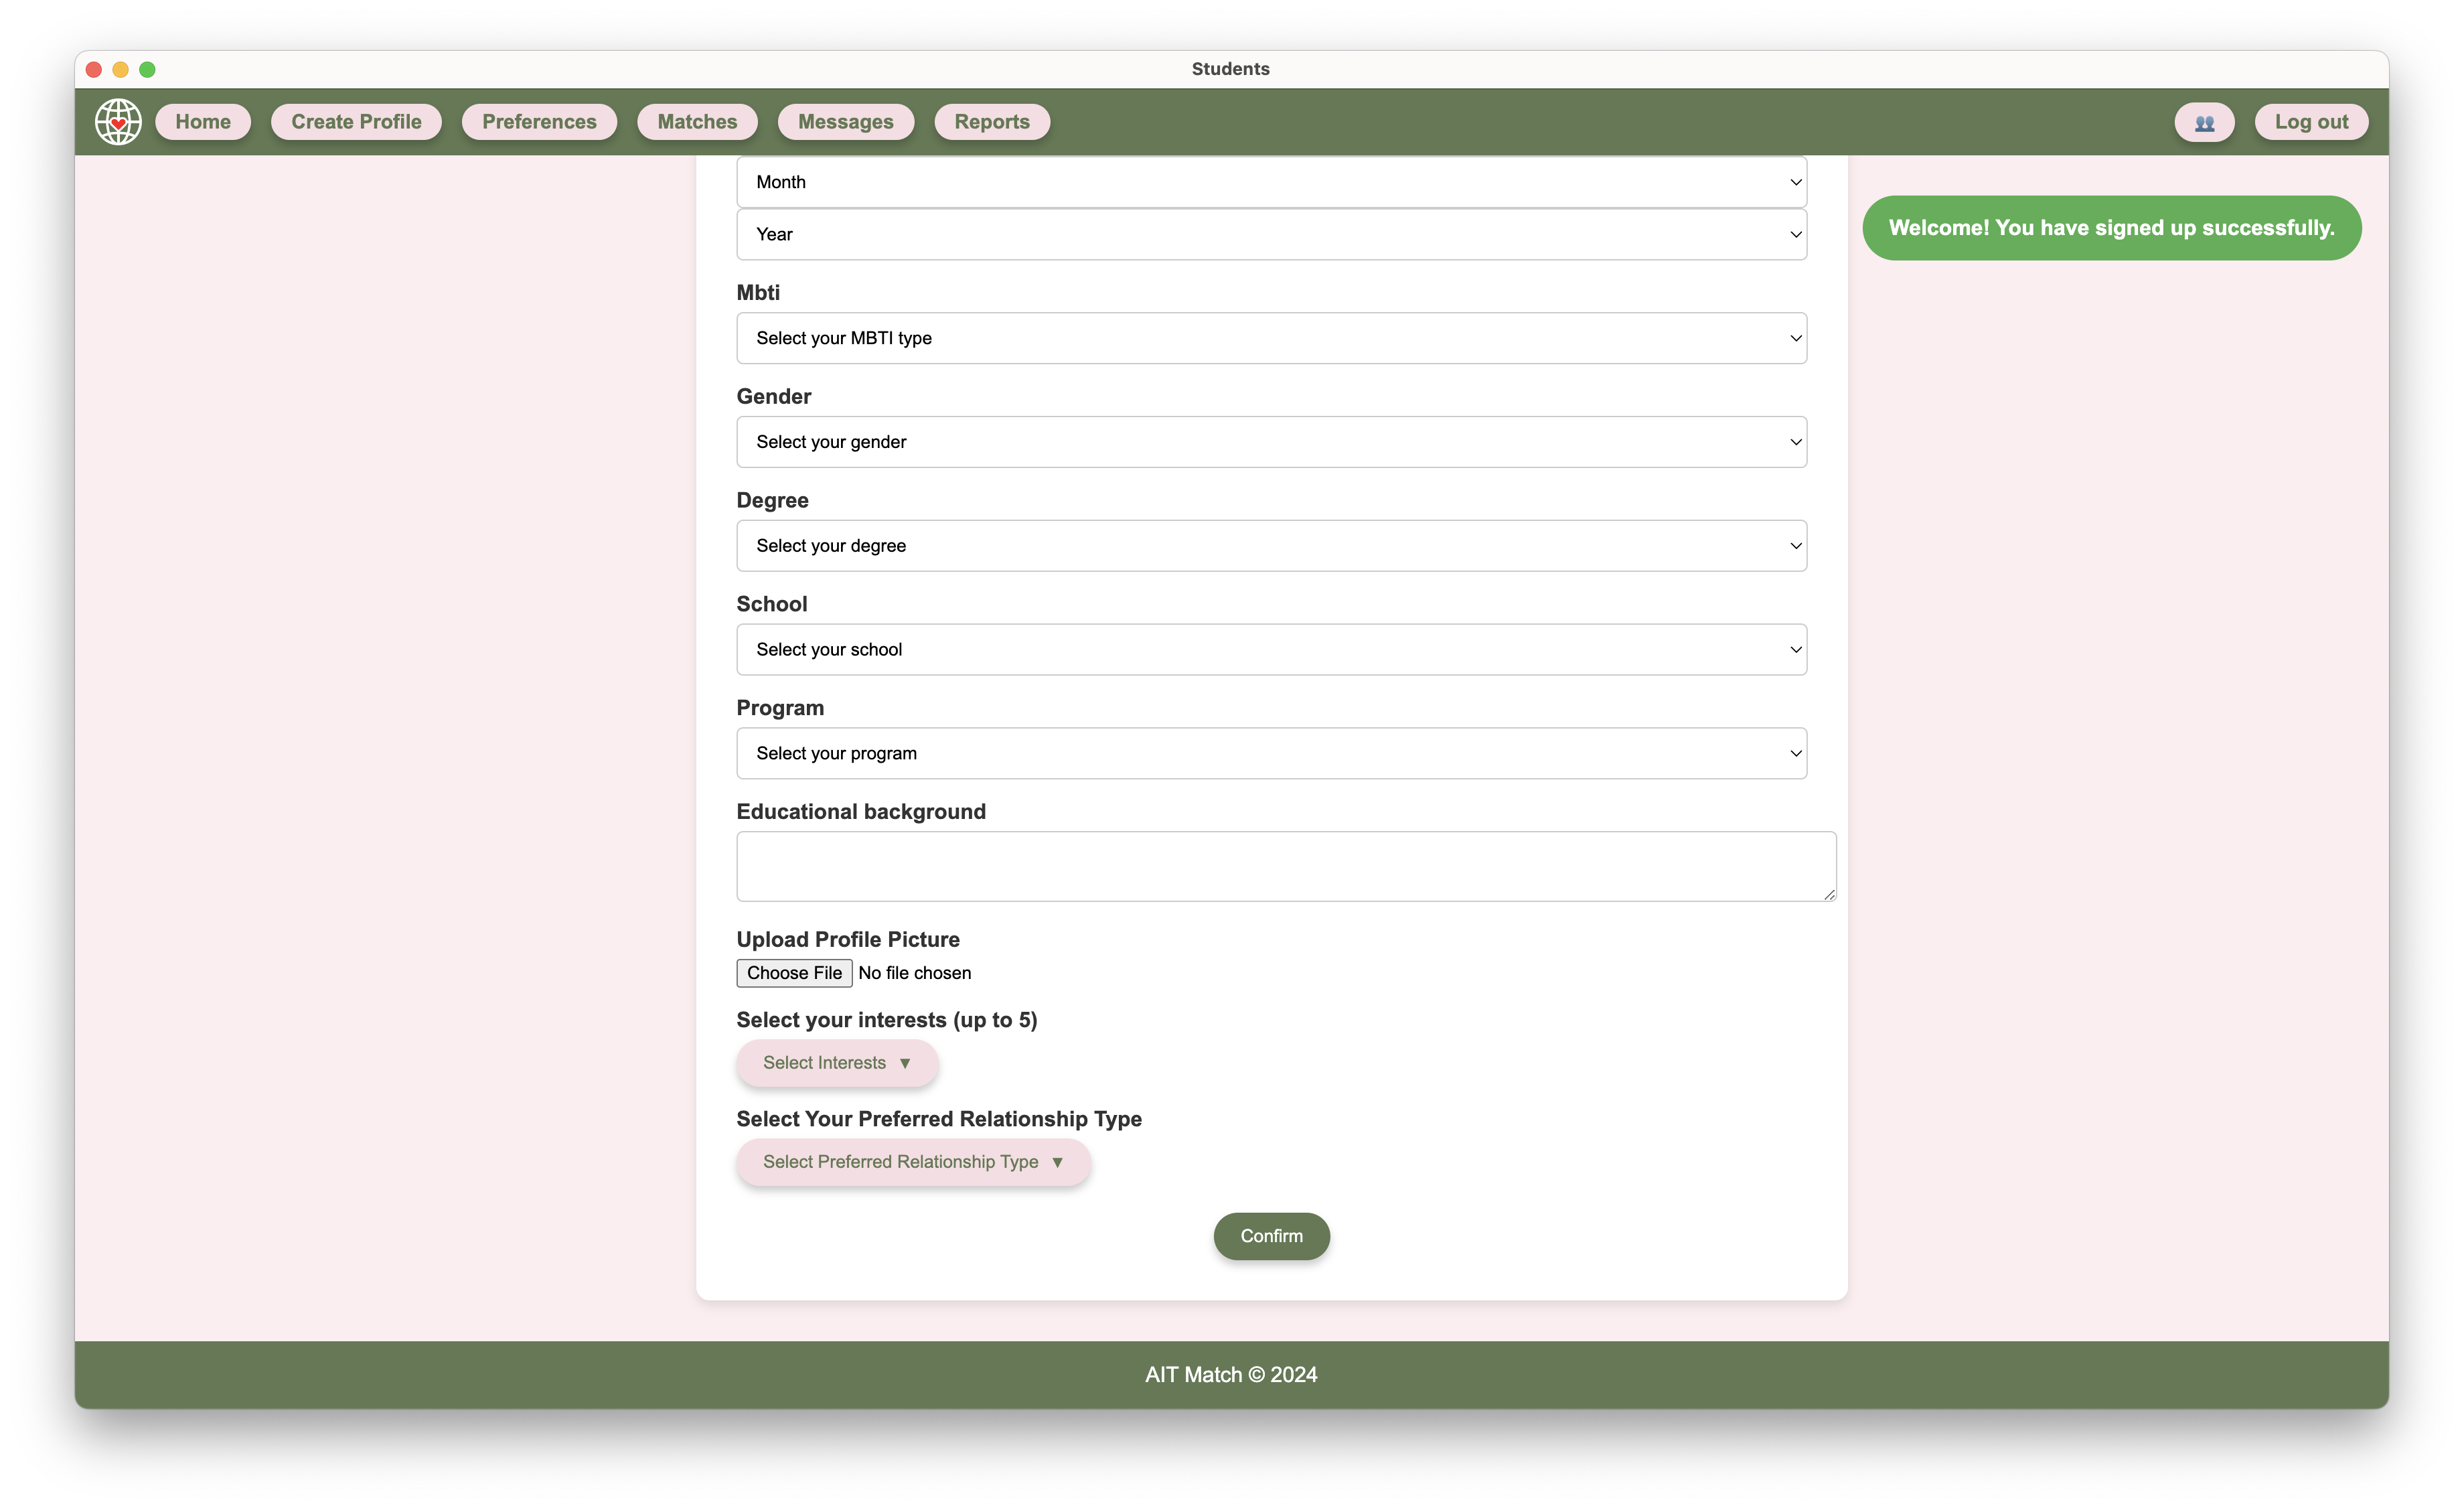
\includegraphics[width=5in]{figures/results/profiles/create-profile-page2.png} 
                \caption{Profile Creation Page (Continued).}
                \label{fig:create-profile-page2}
            \end{figure}

        \newpage
        \subsection{Profile: Validation of Profile Creation}
        \begin{figure}[h]
                \centering
                \captionsetup{justification=centering, singlelinecheck=false, labelsep=space}
                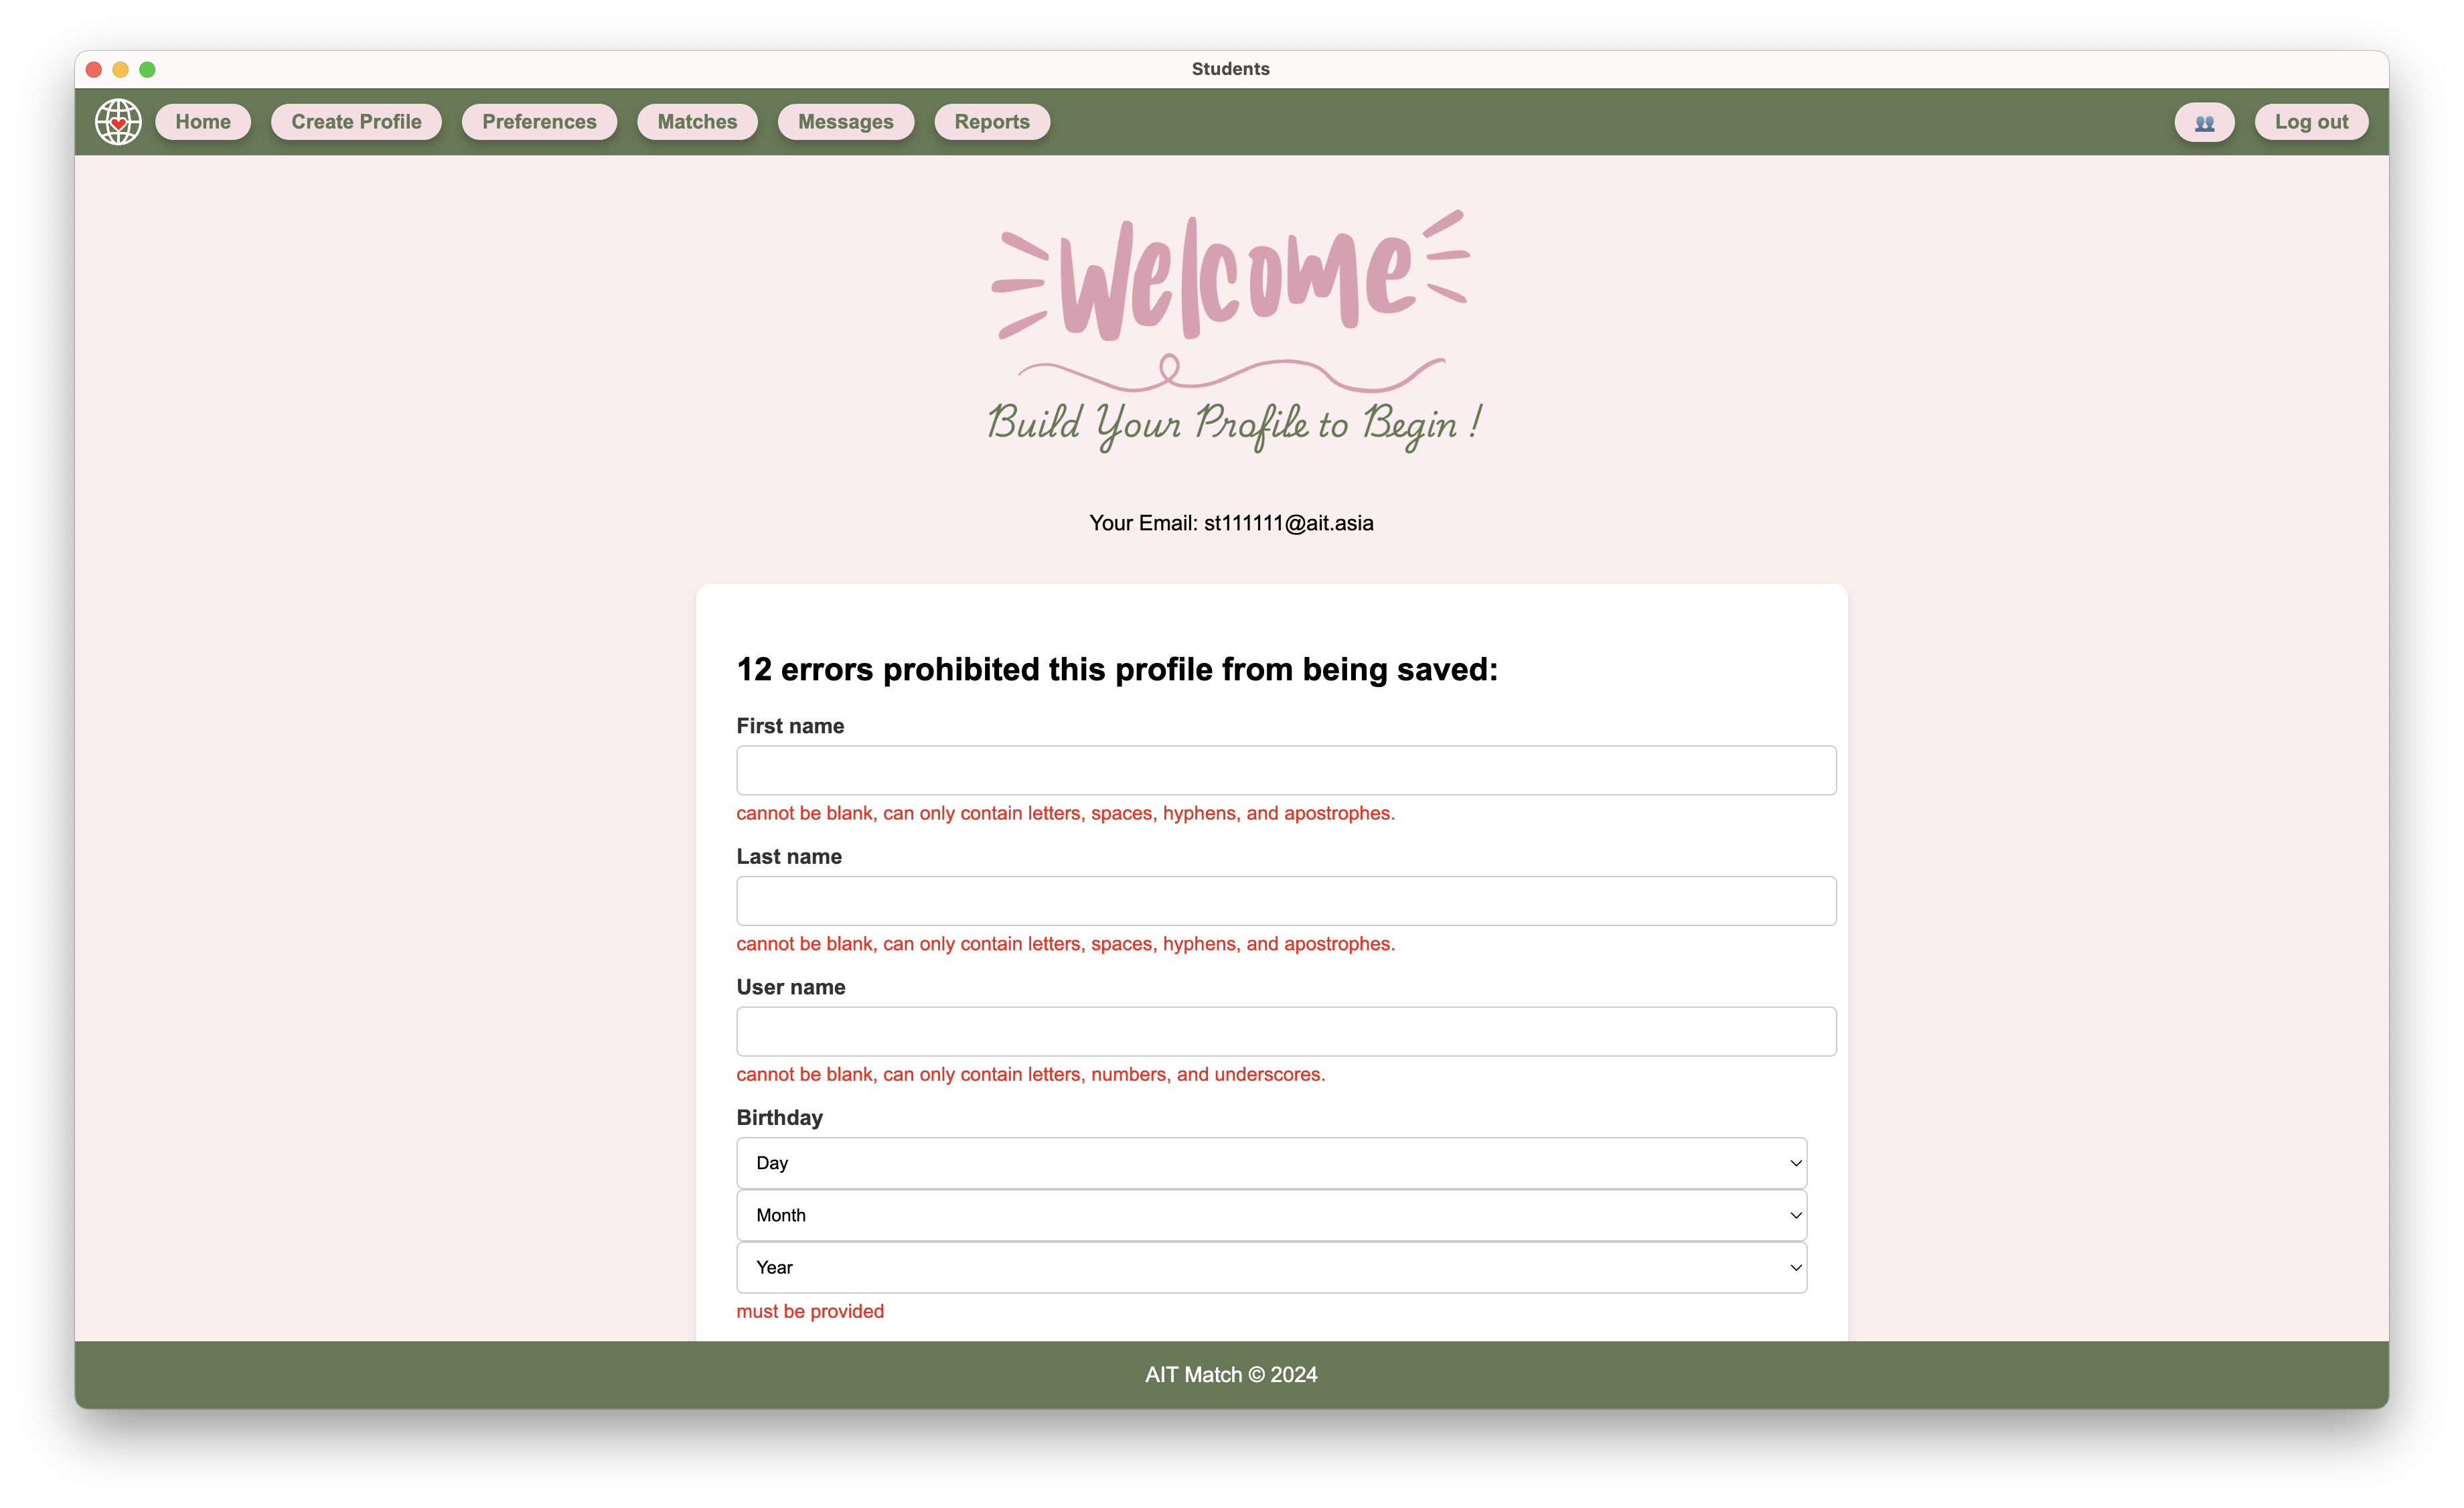
\includegraphics[width=5in]{figures/results/profiles/create-profile-error.png} 
                \caption{Validation of Profile Creation.}
                \label{fig:create-profile-error}
            \end{figure}

        \subsection{Profile: Validation of Profile Creation (Continued)}
        \begin{figure}[h]
                \centering
                \captionsetup{justification=centering, singlelinecheck=false, labelsep=space}
                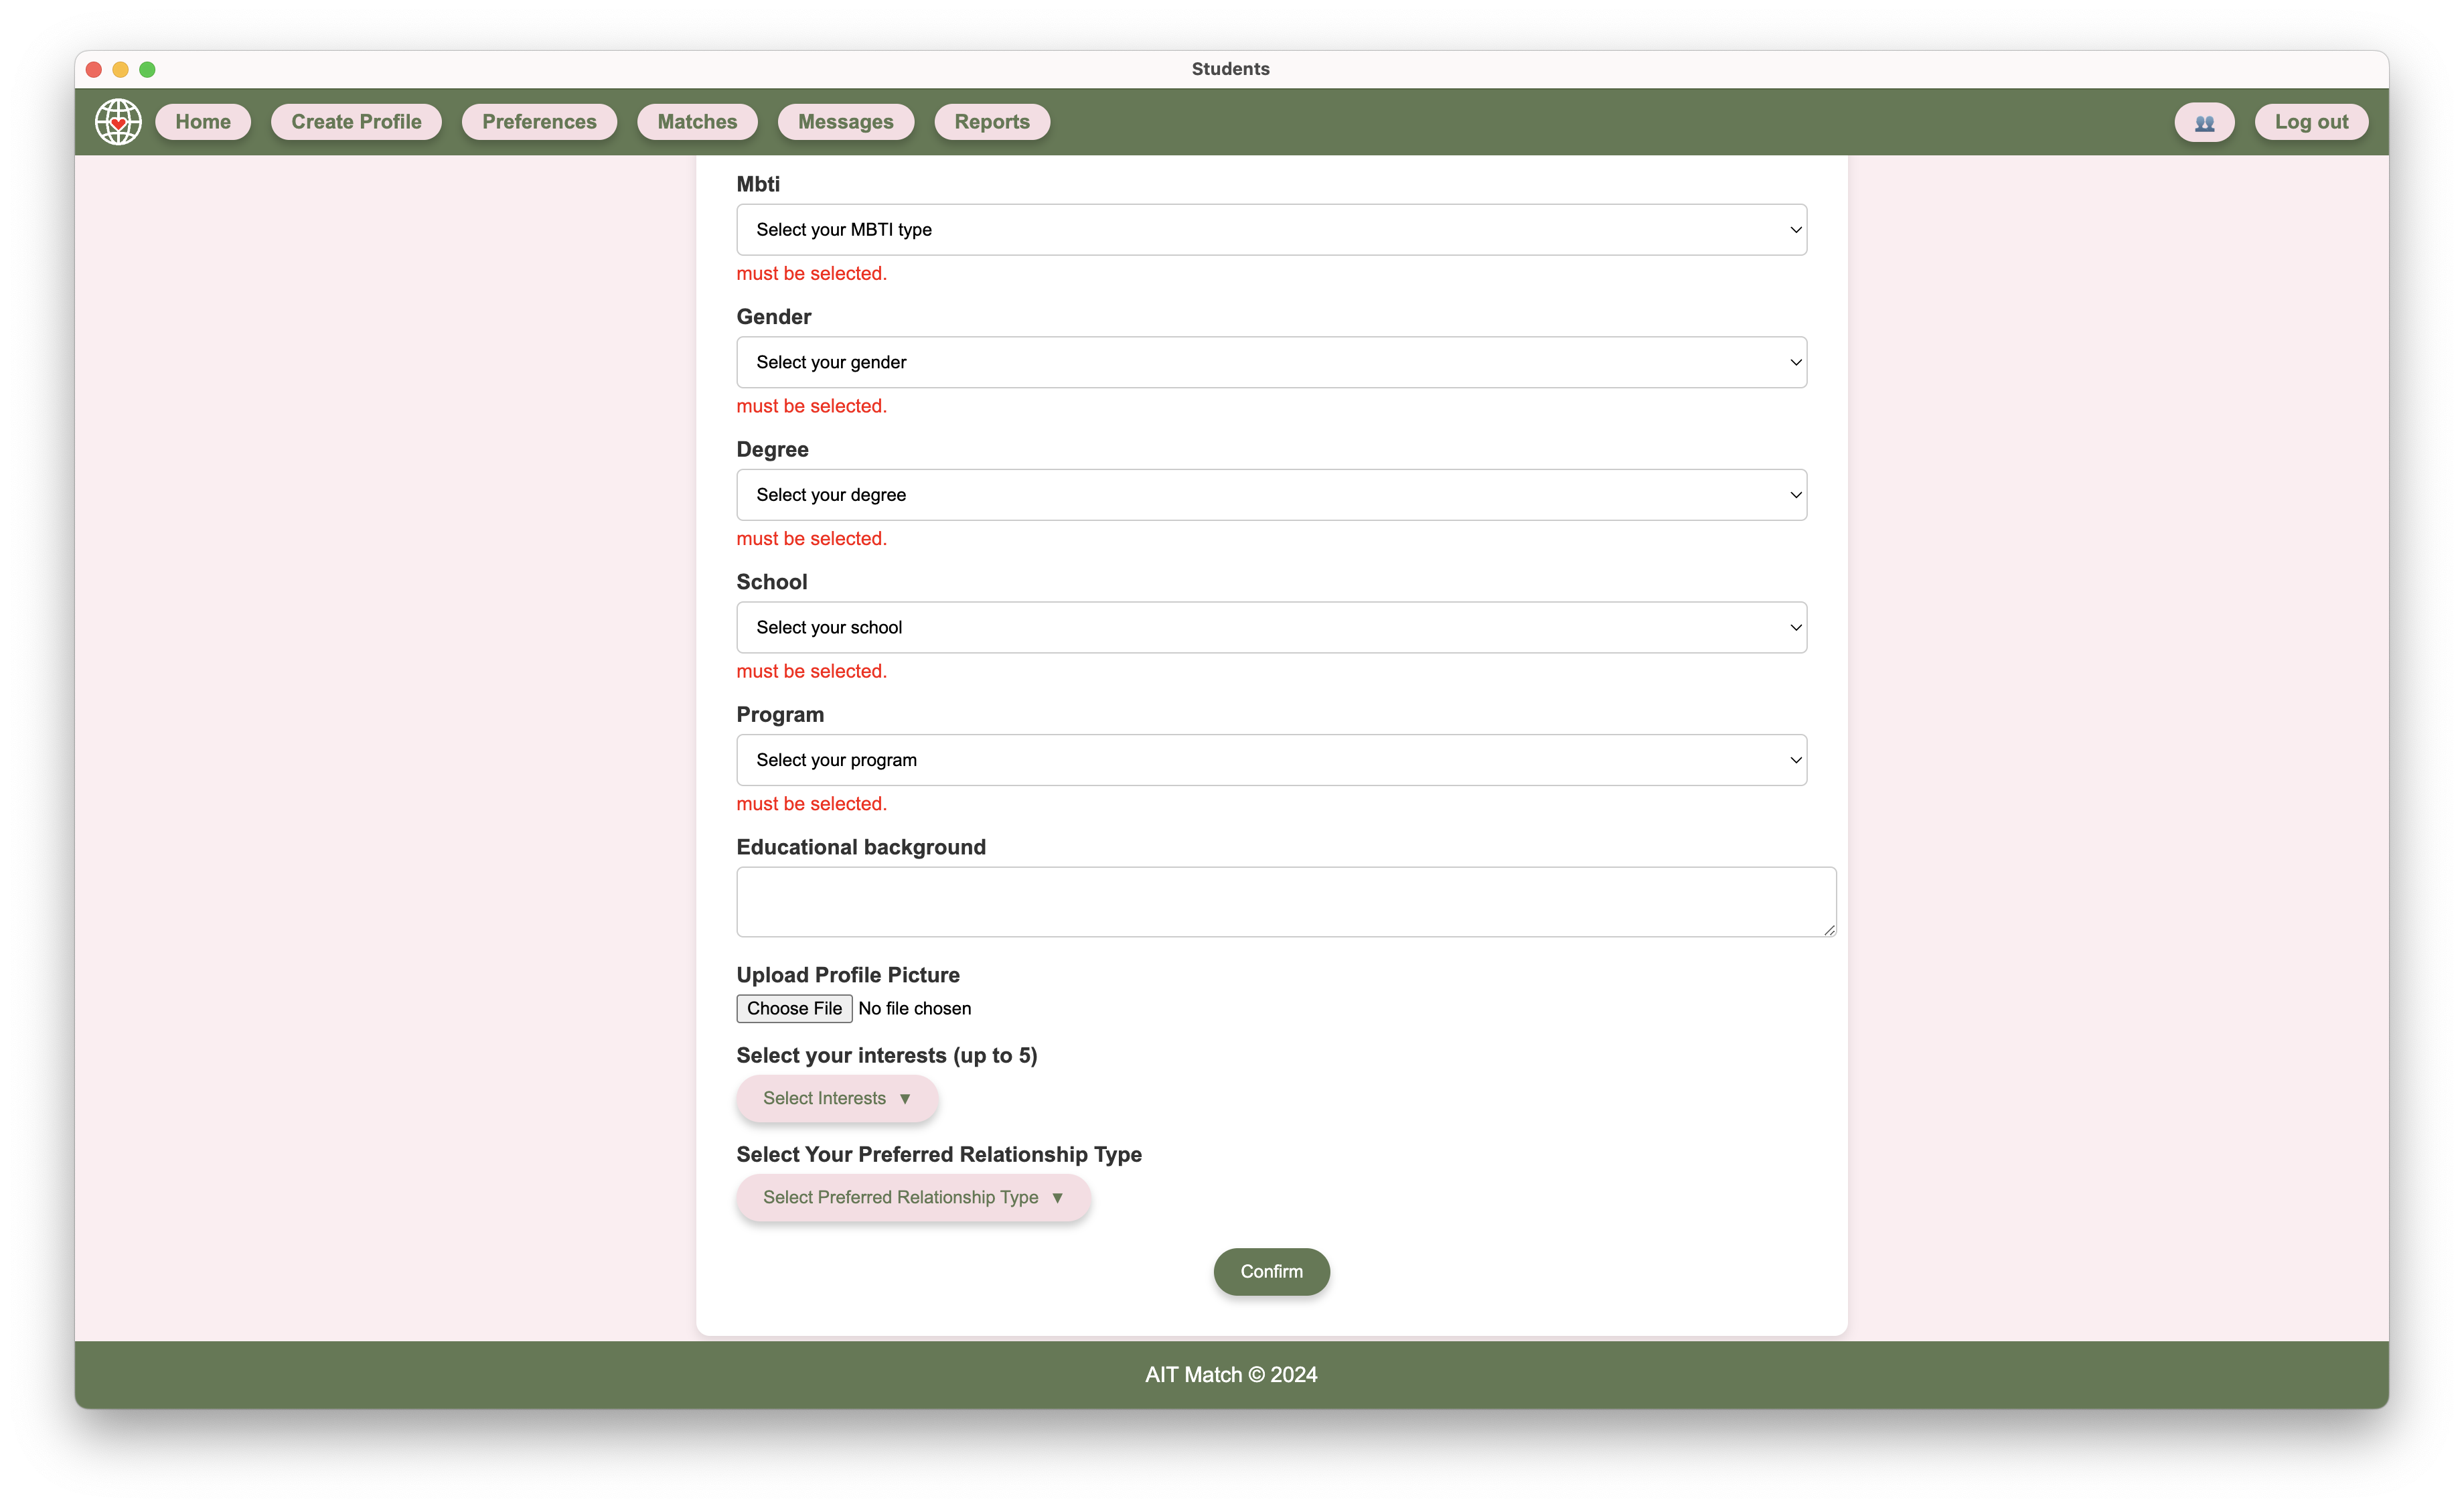
\includegraphics[width=5in]{figures/results/profiles/create-profile-error2.png} 
                \caption{Validation of Profile Creation (Continued).}
                \label{fig:create-profile-error2}
            \end{figure}

        \newpage
        \subsection{Profile: Profile Edit Page}
        \begin{figure}[h]
                \centering
                \captionsetup{justification=centering, singlelinecheck=false, labelsep=space}
                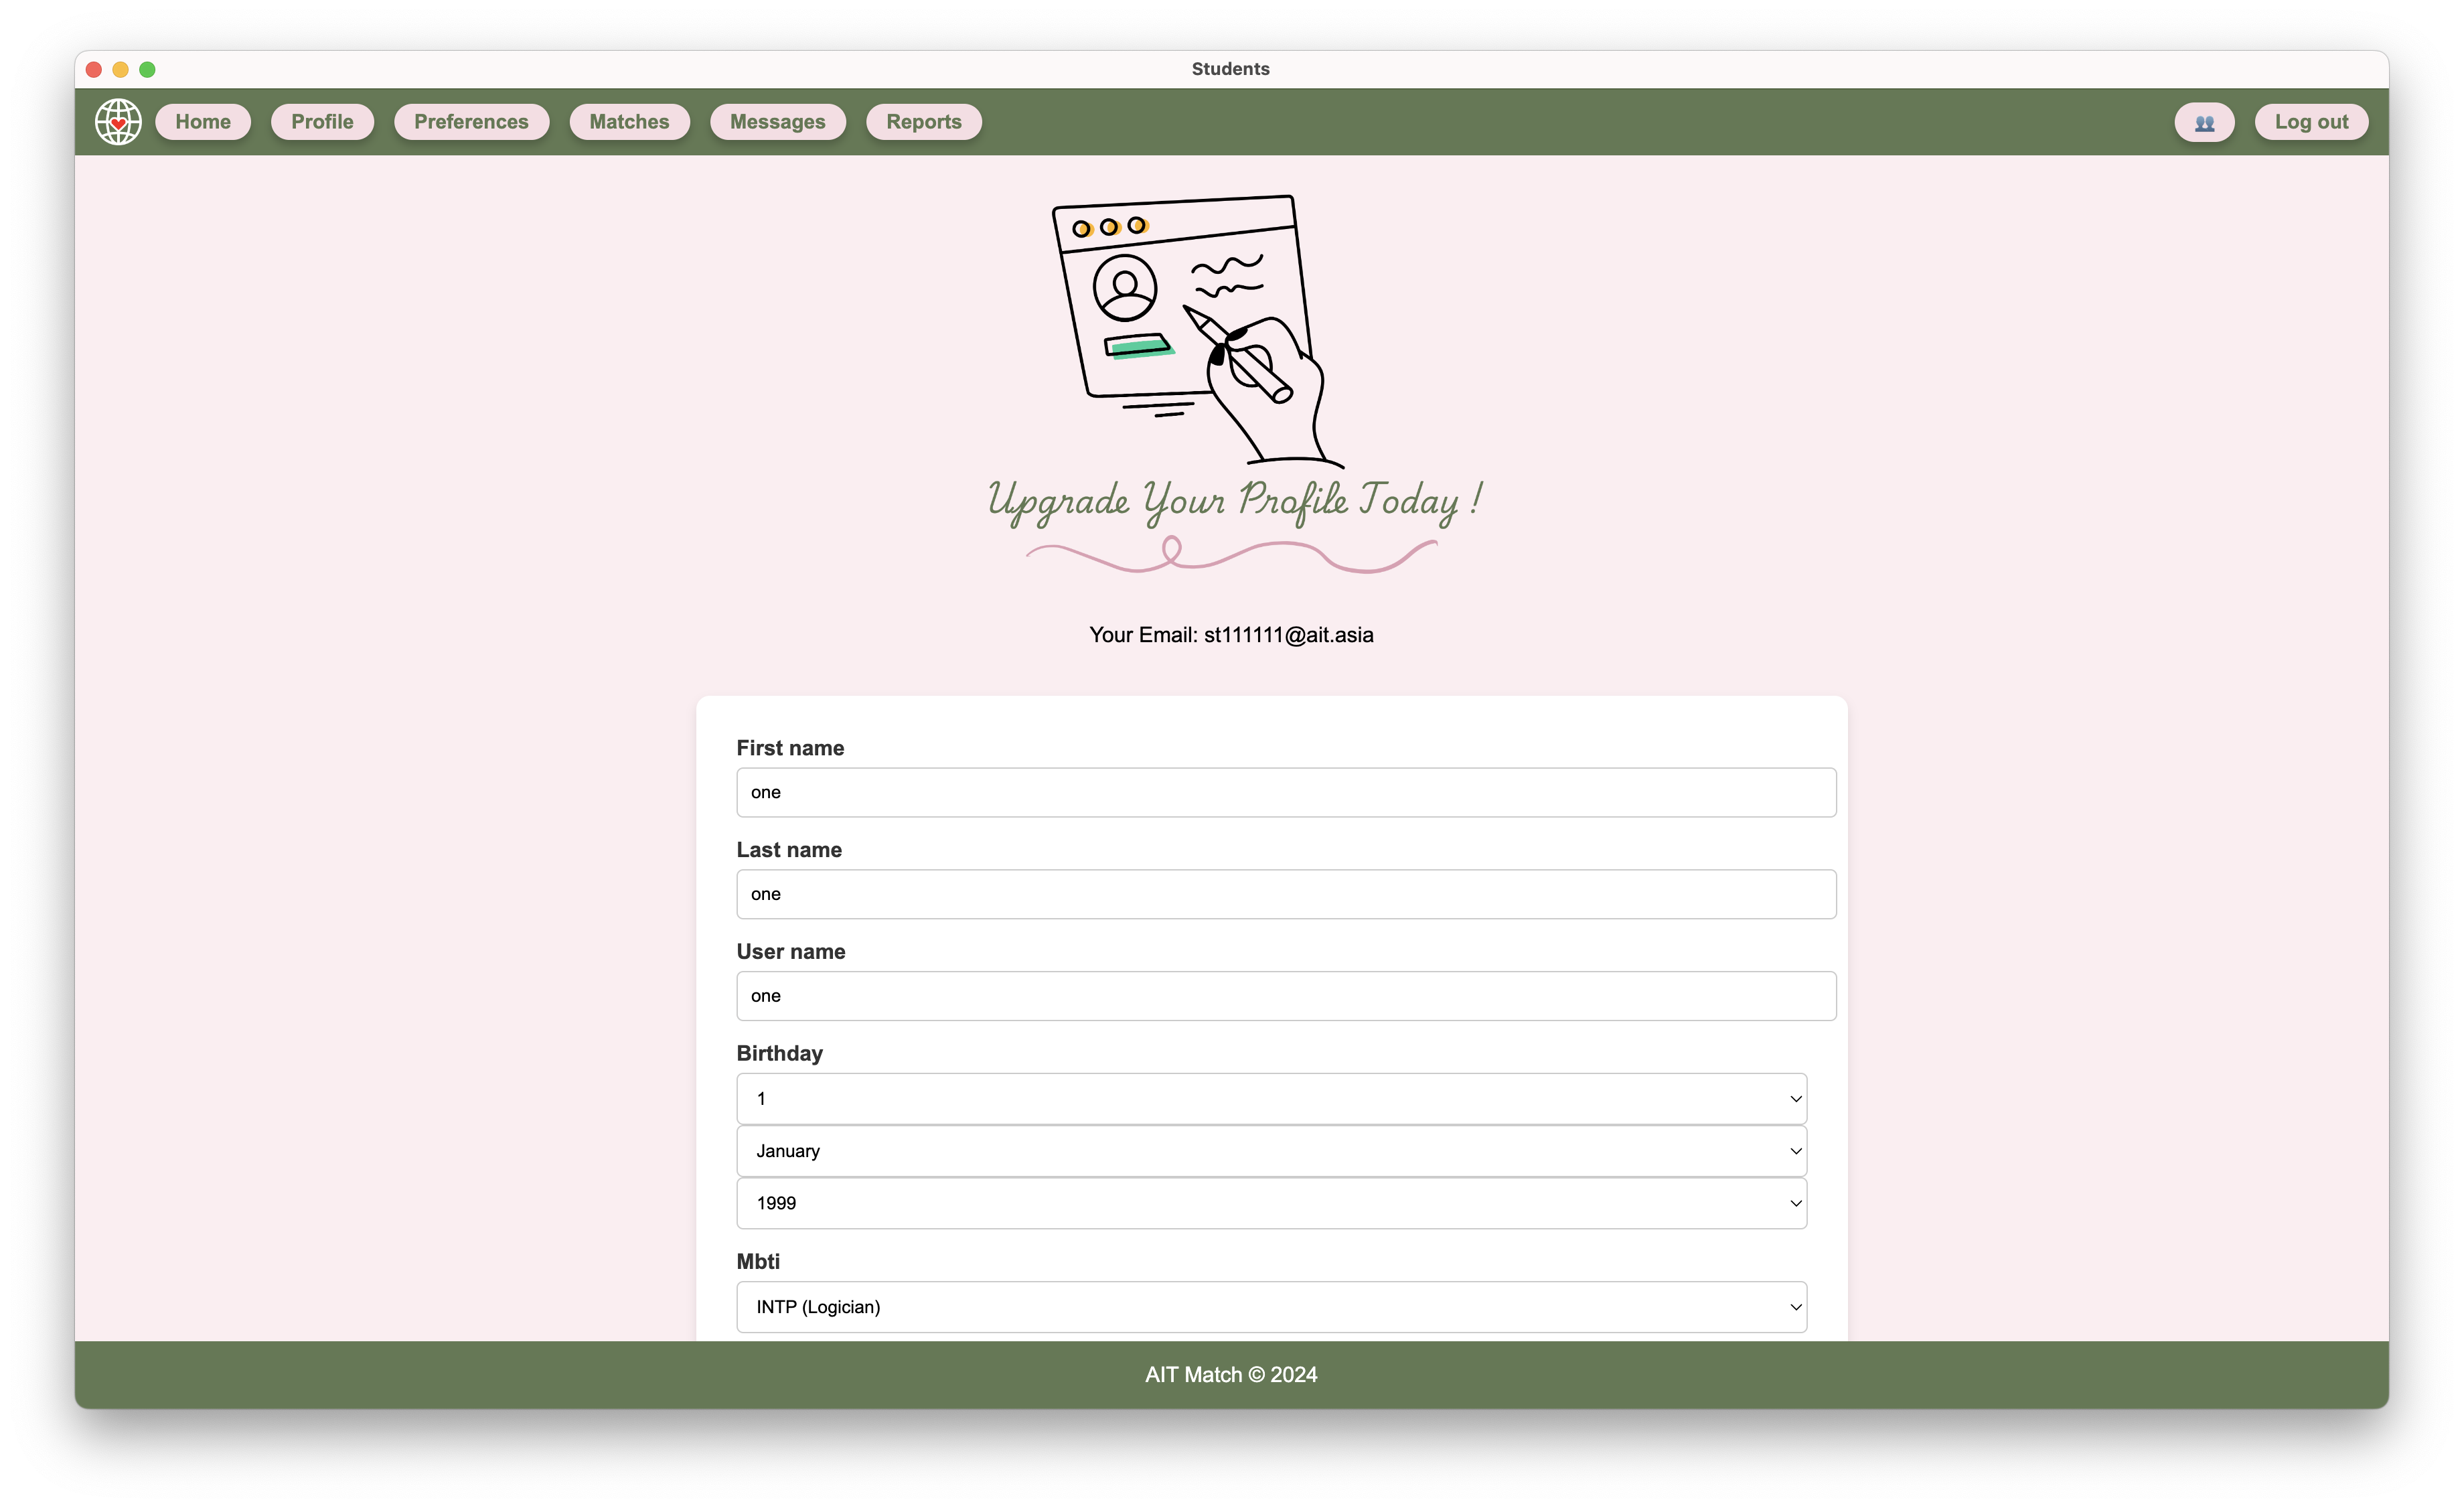
\includegraphics[width=5in]{figures/results/profiles/edit-profile-page.png} 
                \caption{Profile Edit Page.}
                \label{fig:edit-profile-page}
            \end{figure}

        \subsection{Profile: Profile Edit Page (Continued)}
        \begin{figure}[h]
                \centering
                \captionsetup{justification=centering, singlelinecheck=false, labelsep=space}
                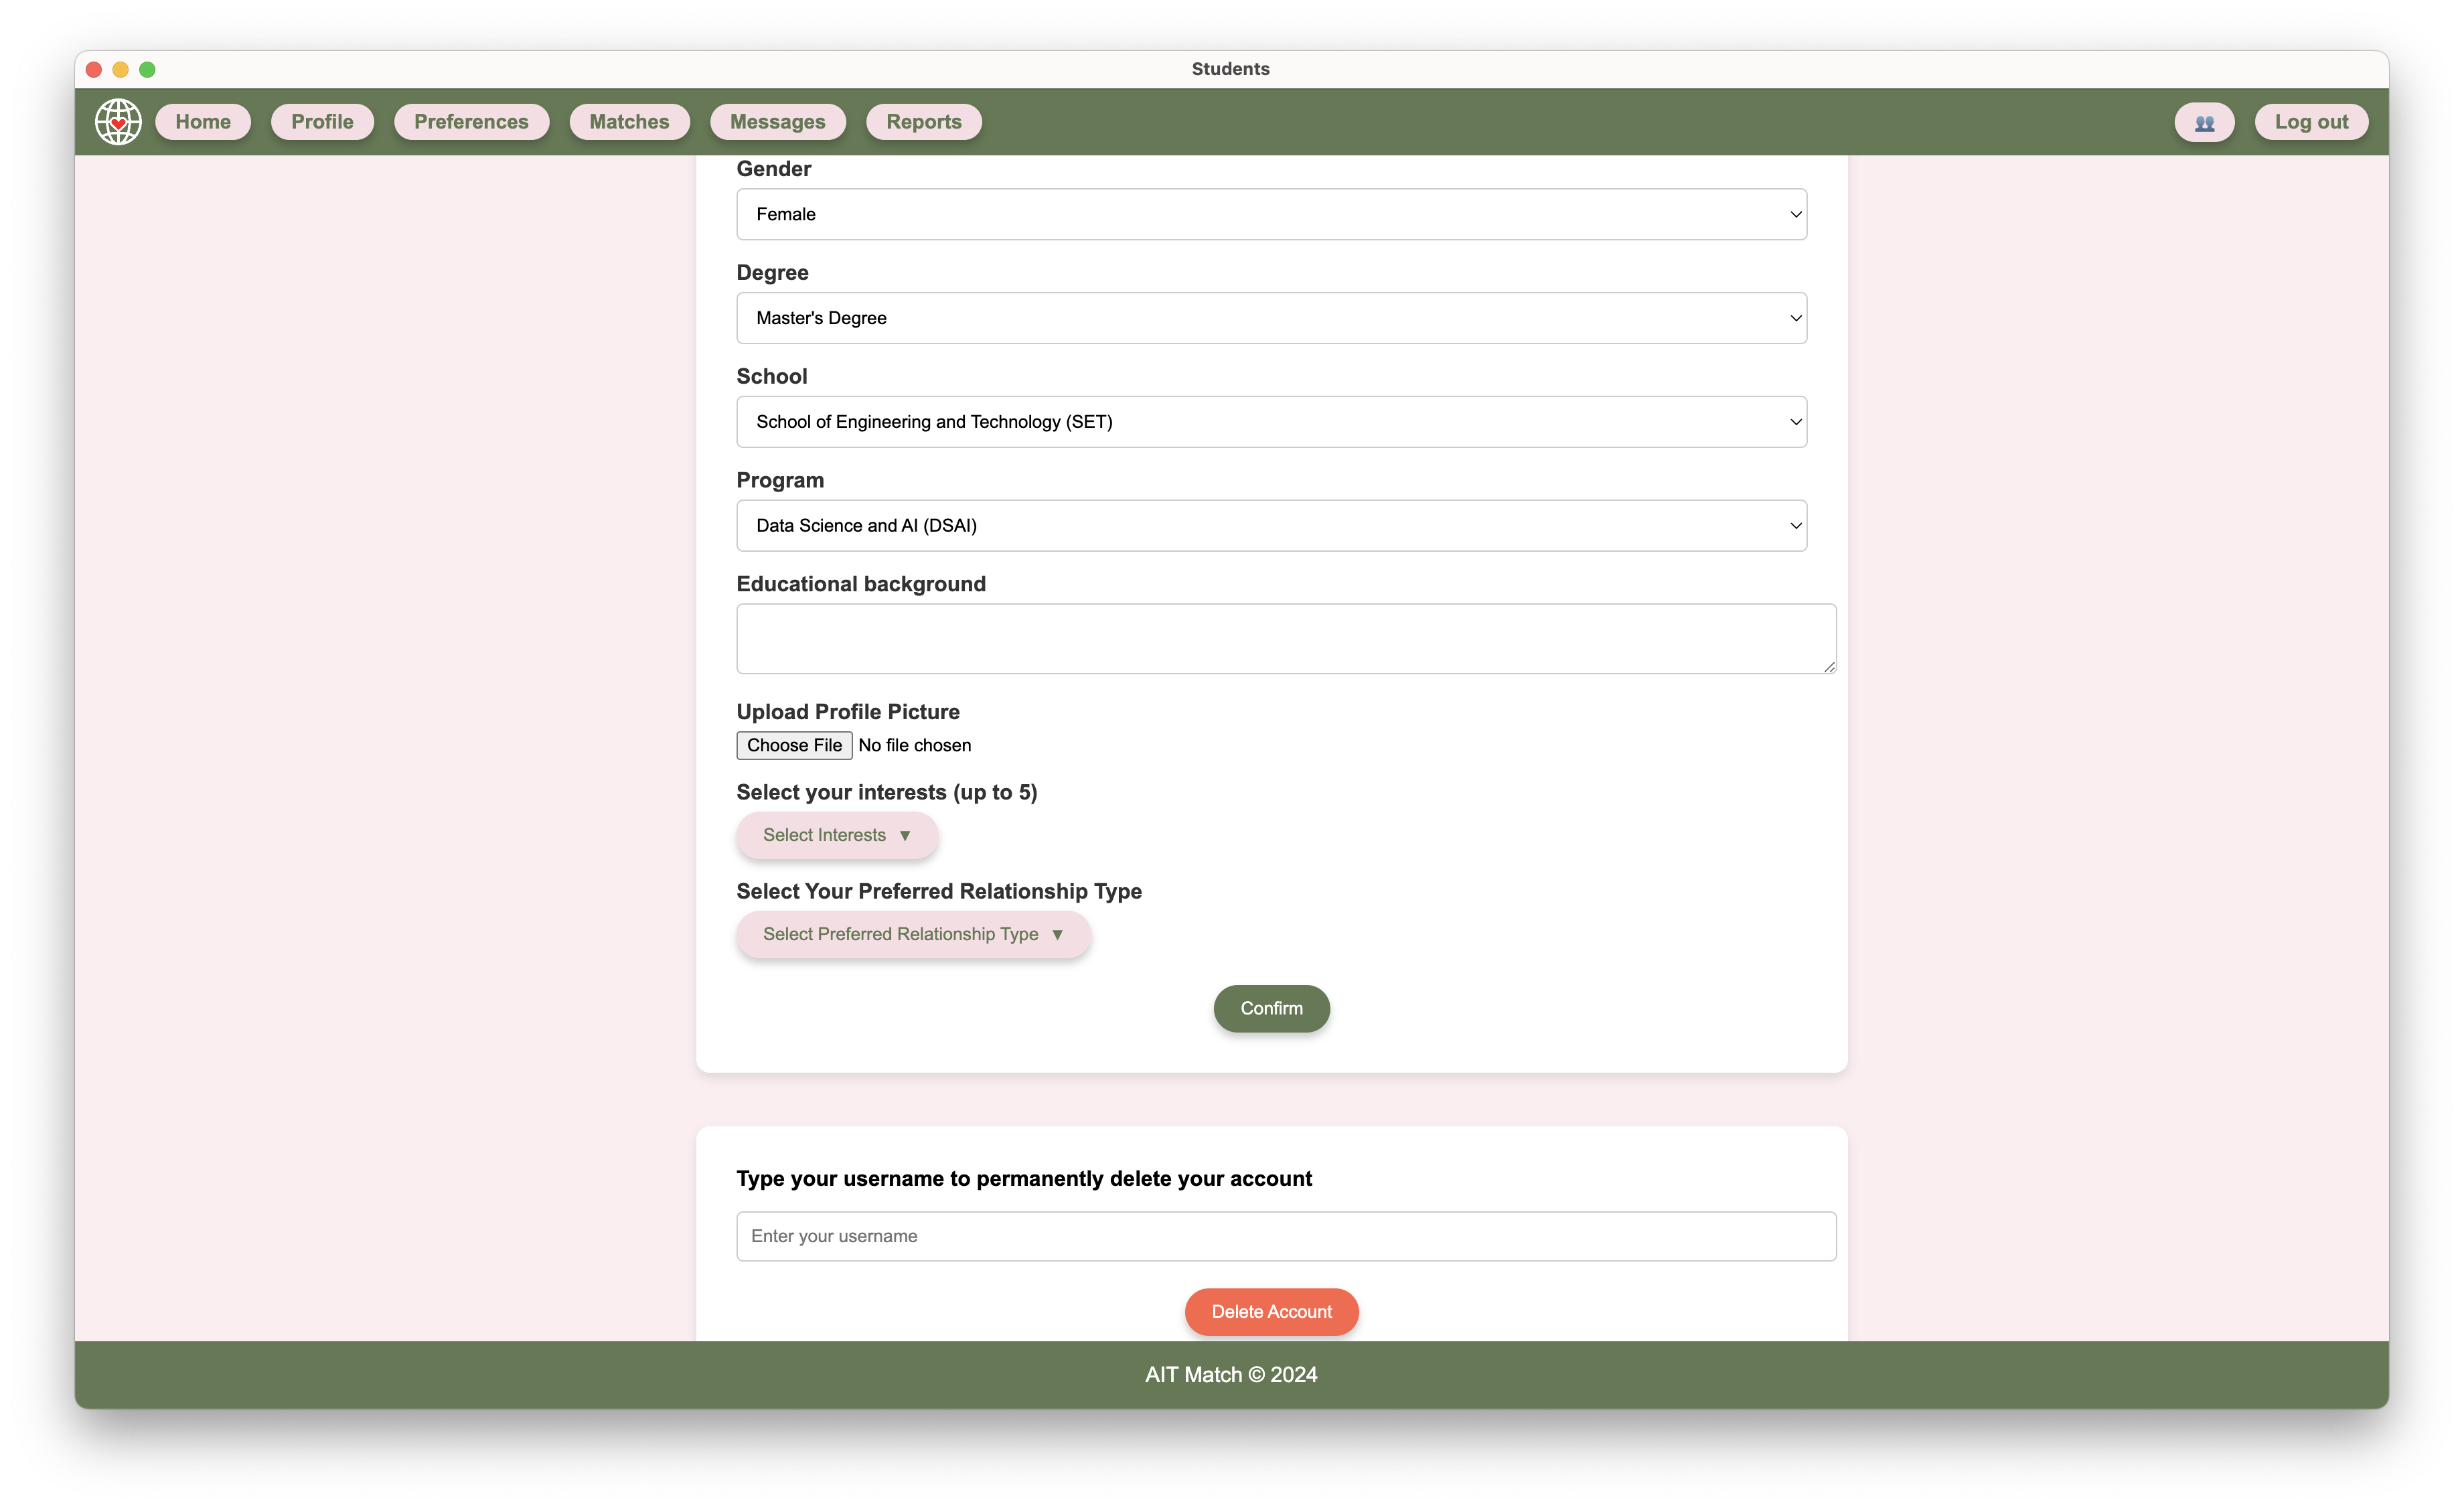
\includegraphics[width=5in]{figures/results/profiles/edit-profile-page2.png} 
                \caption{Profile Edit Page (Continued).}
                \label{fig:edit-profile-page2}
            \end{figure}

        \newpage
        \subsection{Profile: Profile Show Page}
        \begin{figure}[h]
                \centering
                \captionsetup{justification=centering, singlelinecheck=false, labelsep=space}
                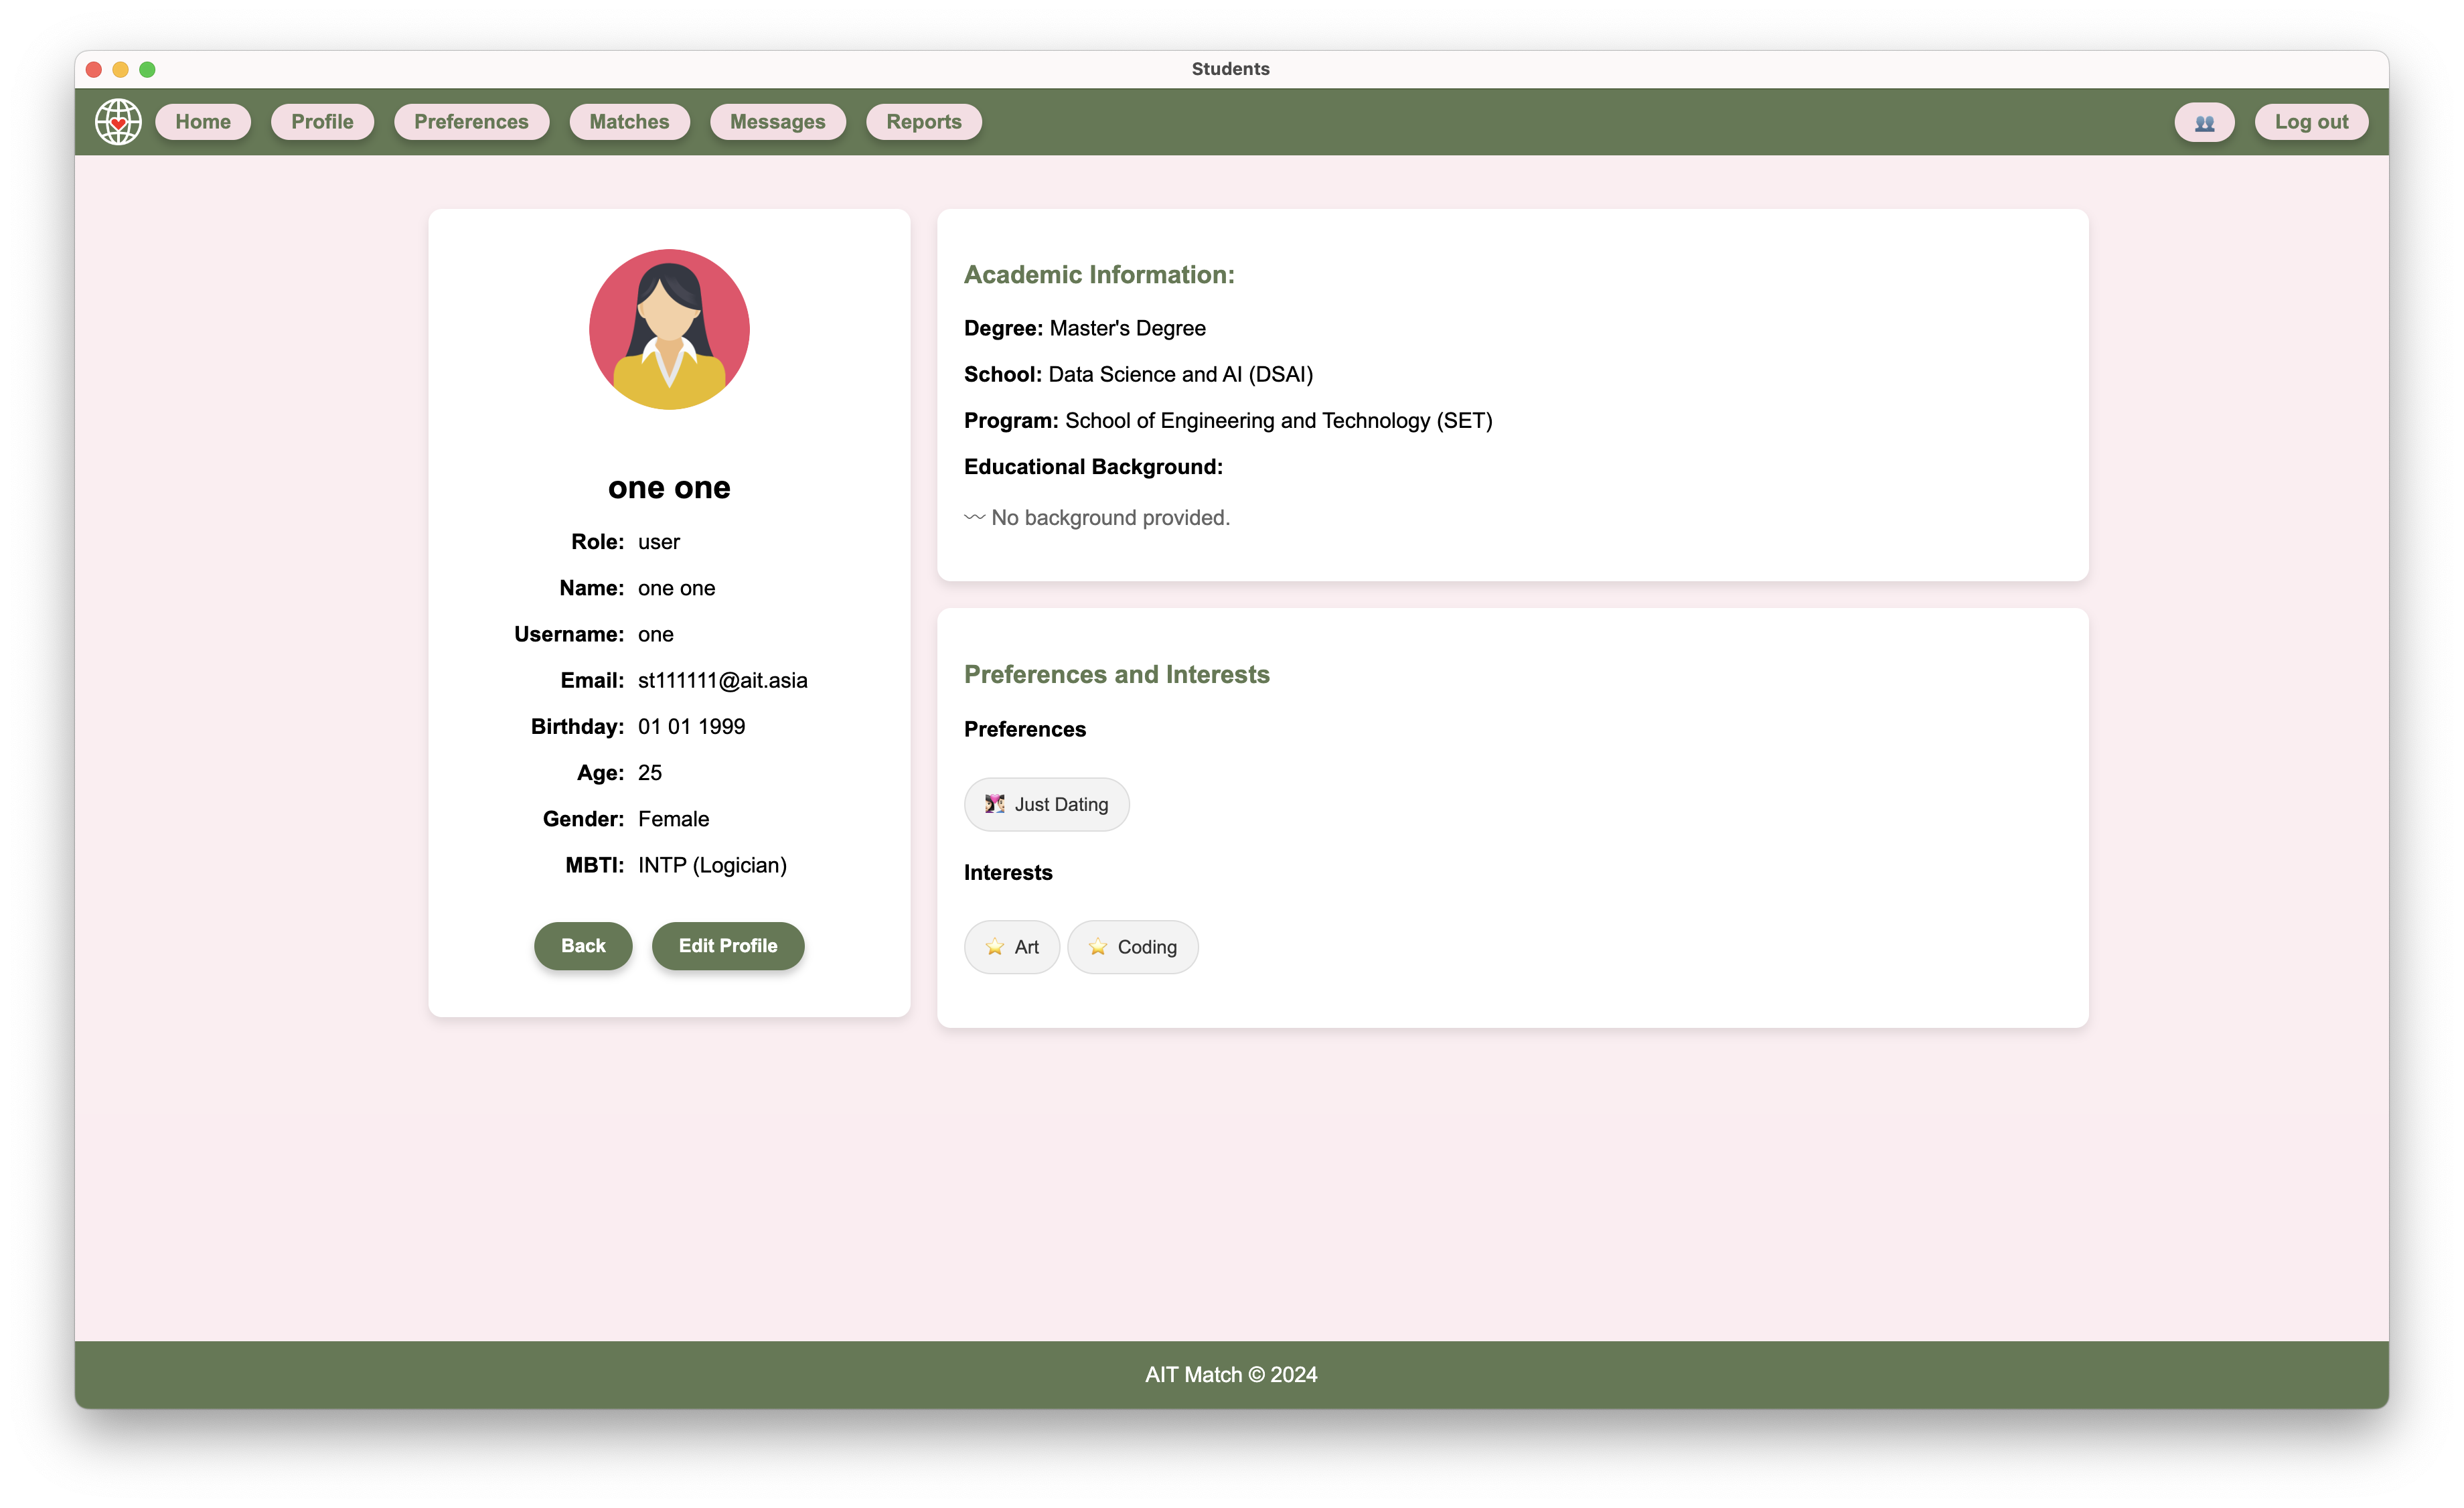
\includegraphics[width=5in]{figures/results/profiles/show-profile-page.png} 
                \caption{Profile Show Page.}
                \label{fig:show-profile-page}
            \end{figure}

        \subsection{Profile: Profile Index Page}
        \begin{figure}[h]
                \centering
                \captionsetup{justification=centering, singlelinecheck=false, labelsep=space}
                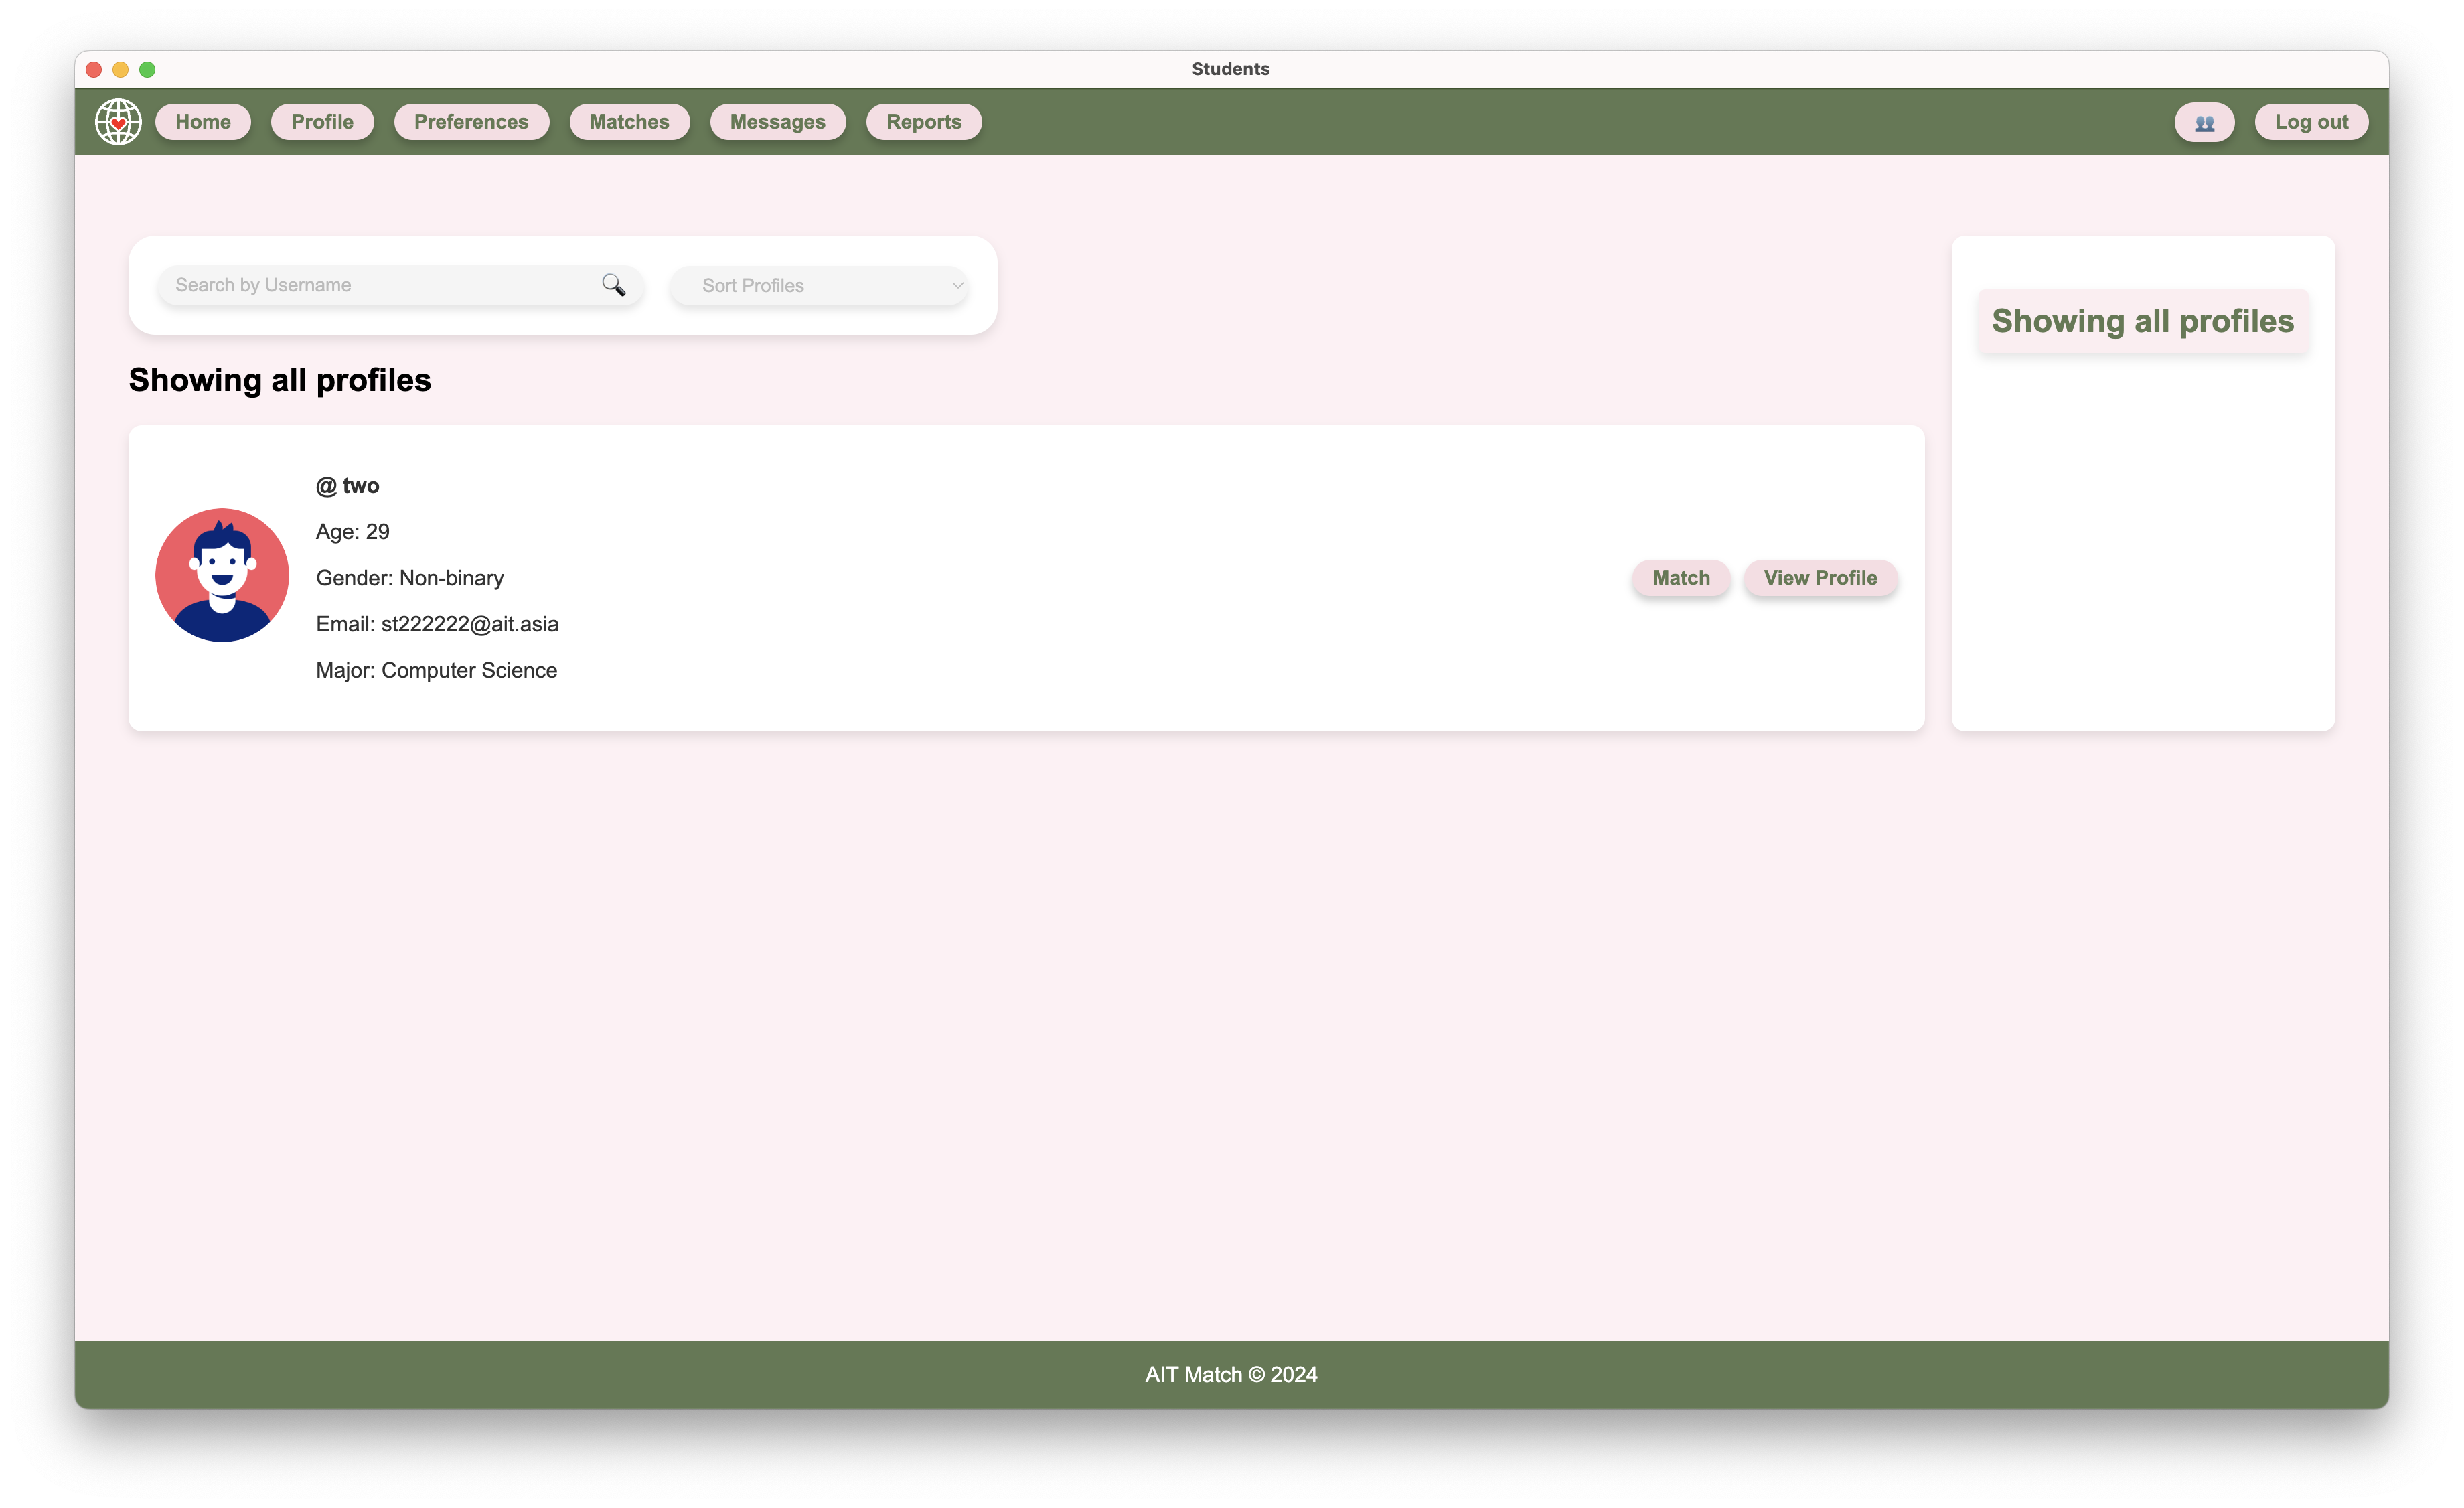
\includegraphics[width=5in]{figures/results/profiles/profile-index-page.png} 
                \caption{Profile Index Page.}
                \label{fig:profile-index-page}
            \end{figure}
% ------------------------------------------------- %
        \newpage
        \subsection{Preference: Preference Setup Page}
        \begin{figure}[h]
                \centering
                \captionsetup{justification=centering, singlelinecheck=false, labelsep=space}
                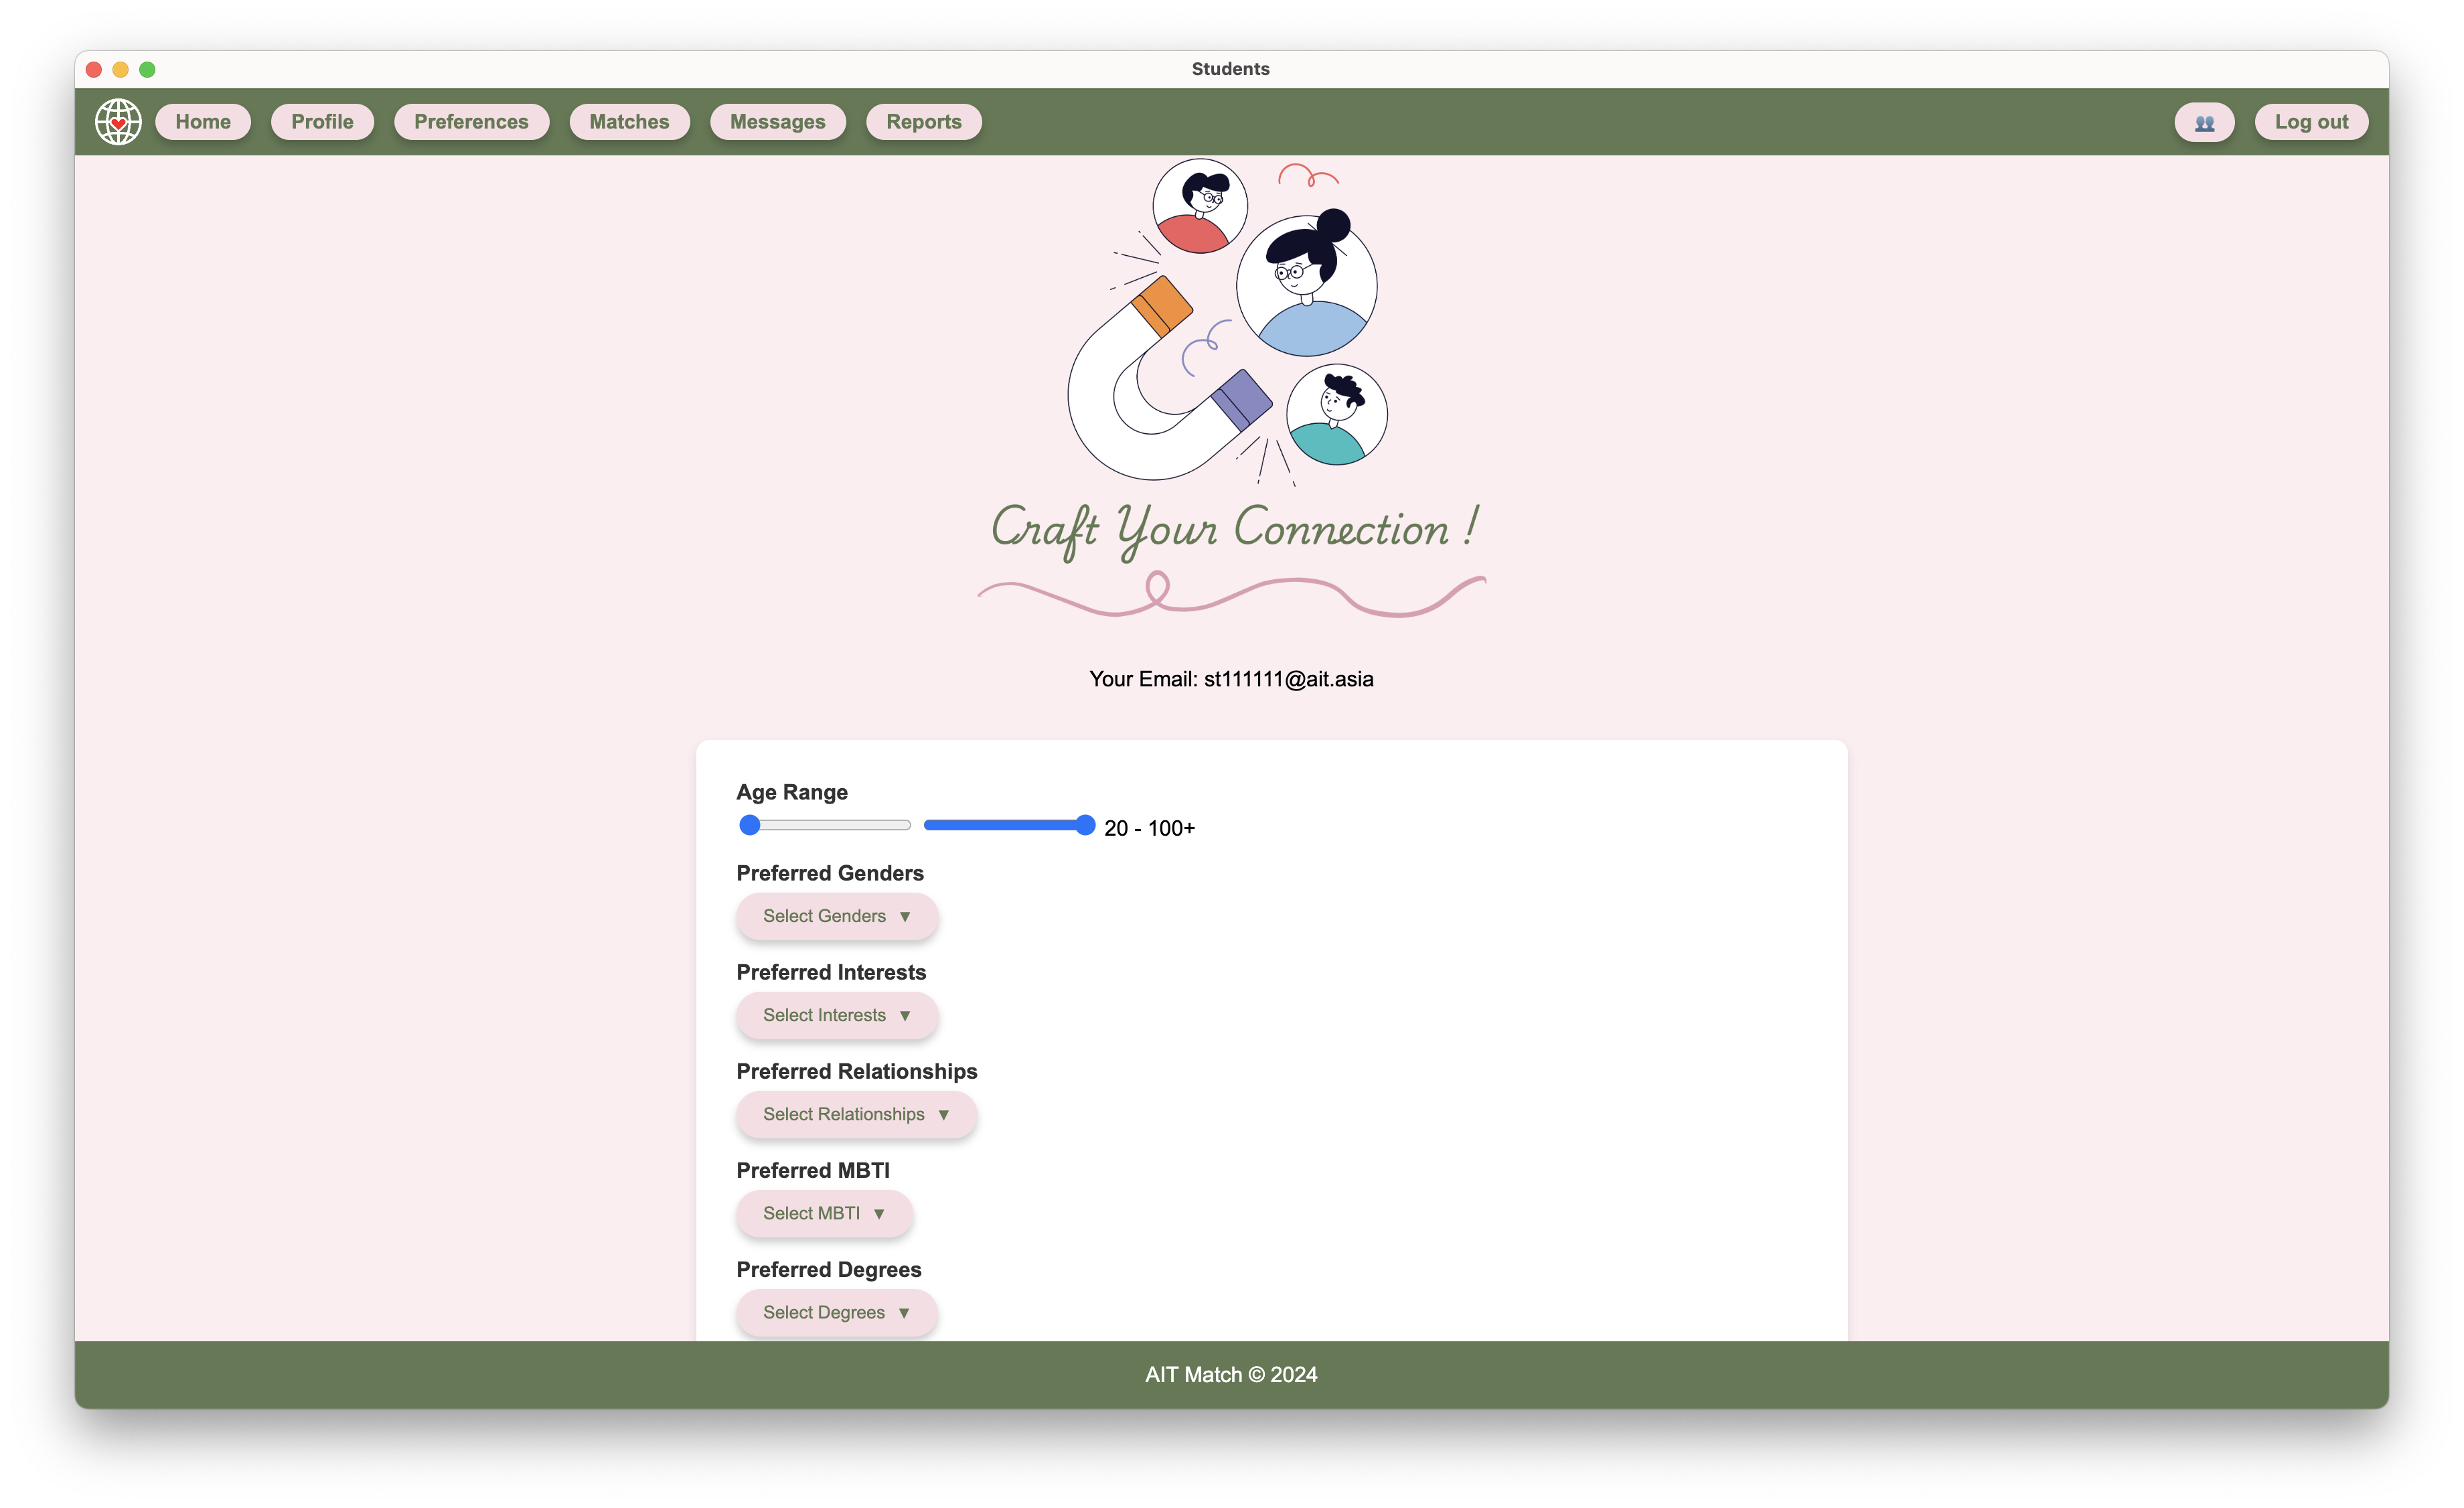
\includegraphics[width=5in]{figures/results/preferences/set-preference-page.png} 
                \caption{Preference Setup Page.}
                \label{fig:set-preference-page-2}
            \end{figure}

        \subsection{Preference: Preference Setup Page (Continued)}
        \begin{figure}[h]
                \centering
                \captionsetup{justification=centering, singlelinecheck=false, labelsep=space}
                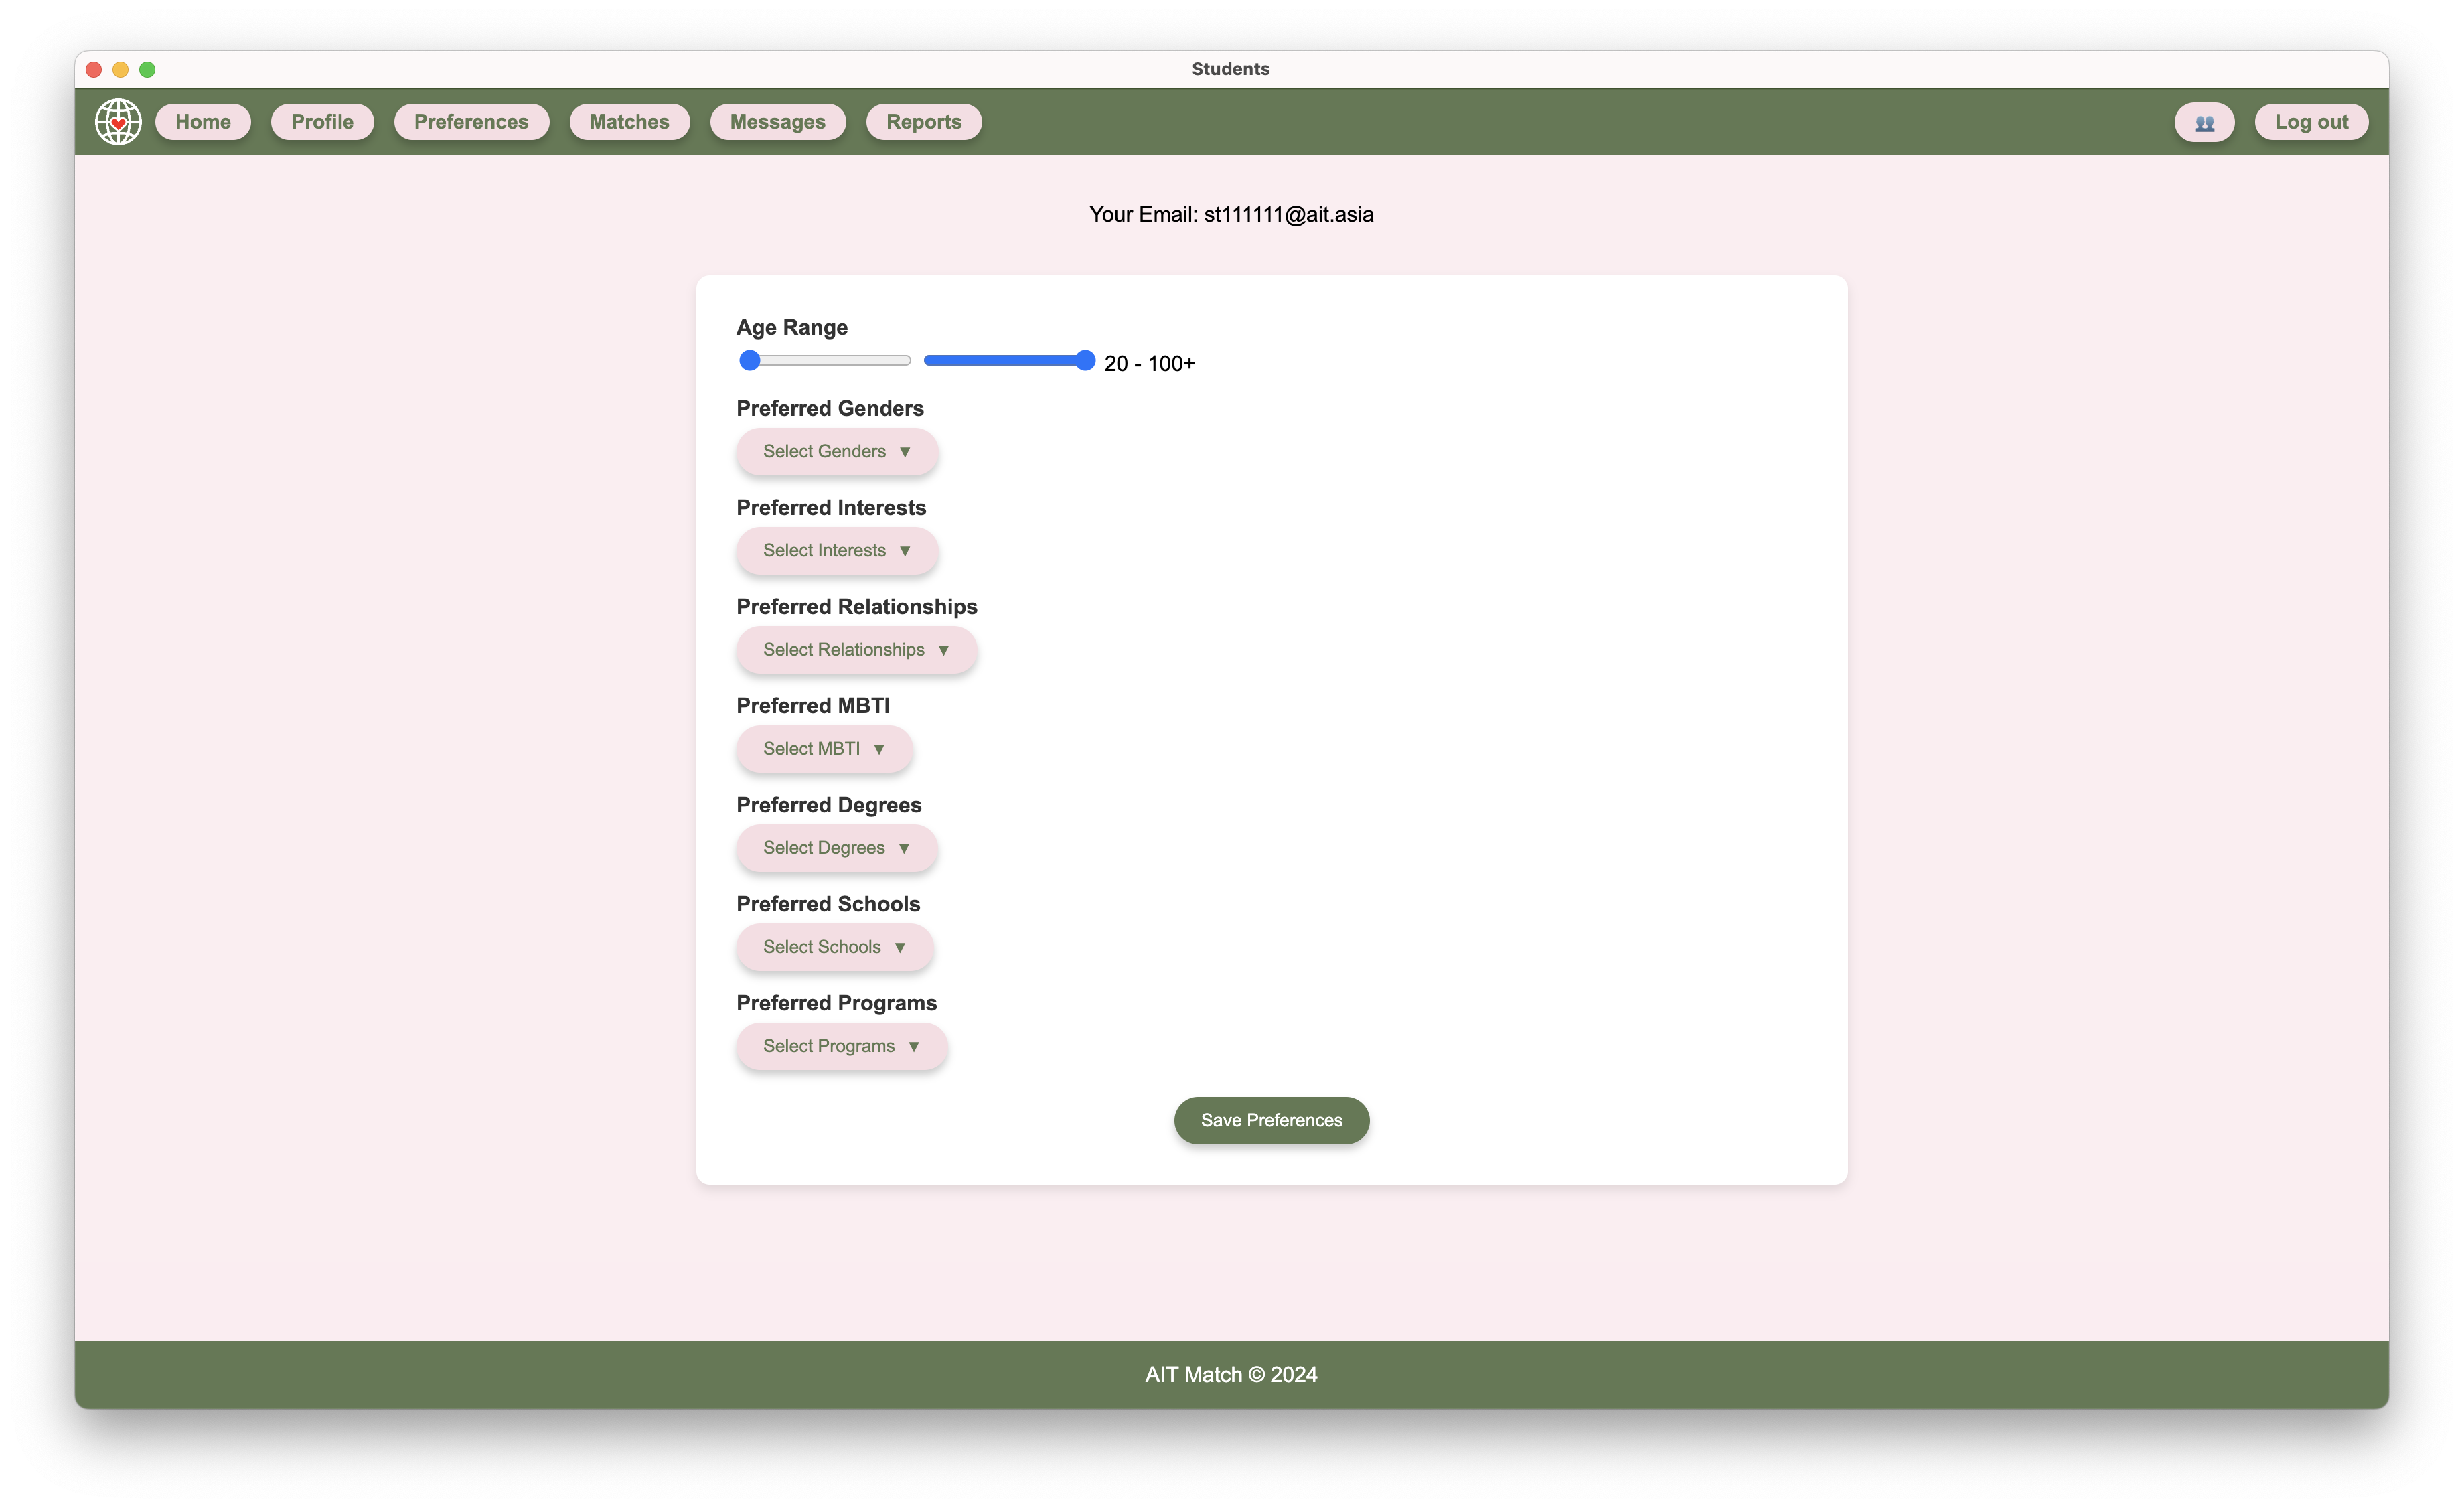
\includegraphics[width=5in]{figures/results/preferences/set-preference-page-2.png} 
                \caption{Preference Setup Page (Continued).}
                \label{fig:set-preference-page-2}
            \end{figure}
% ------------------------------------------------- %
        \newpage
        \subsection{Match: No Match Requests Page}
        \begin{figure}[h]
                \centering
                \captionsetup{justification=centering, singlelinecheck=false, labelsep=space}
                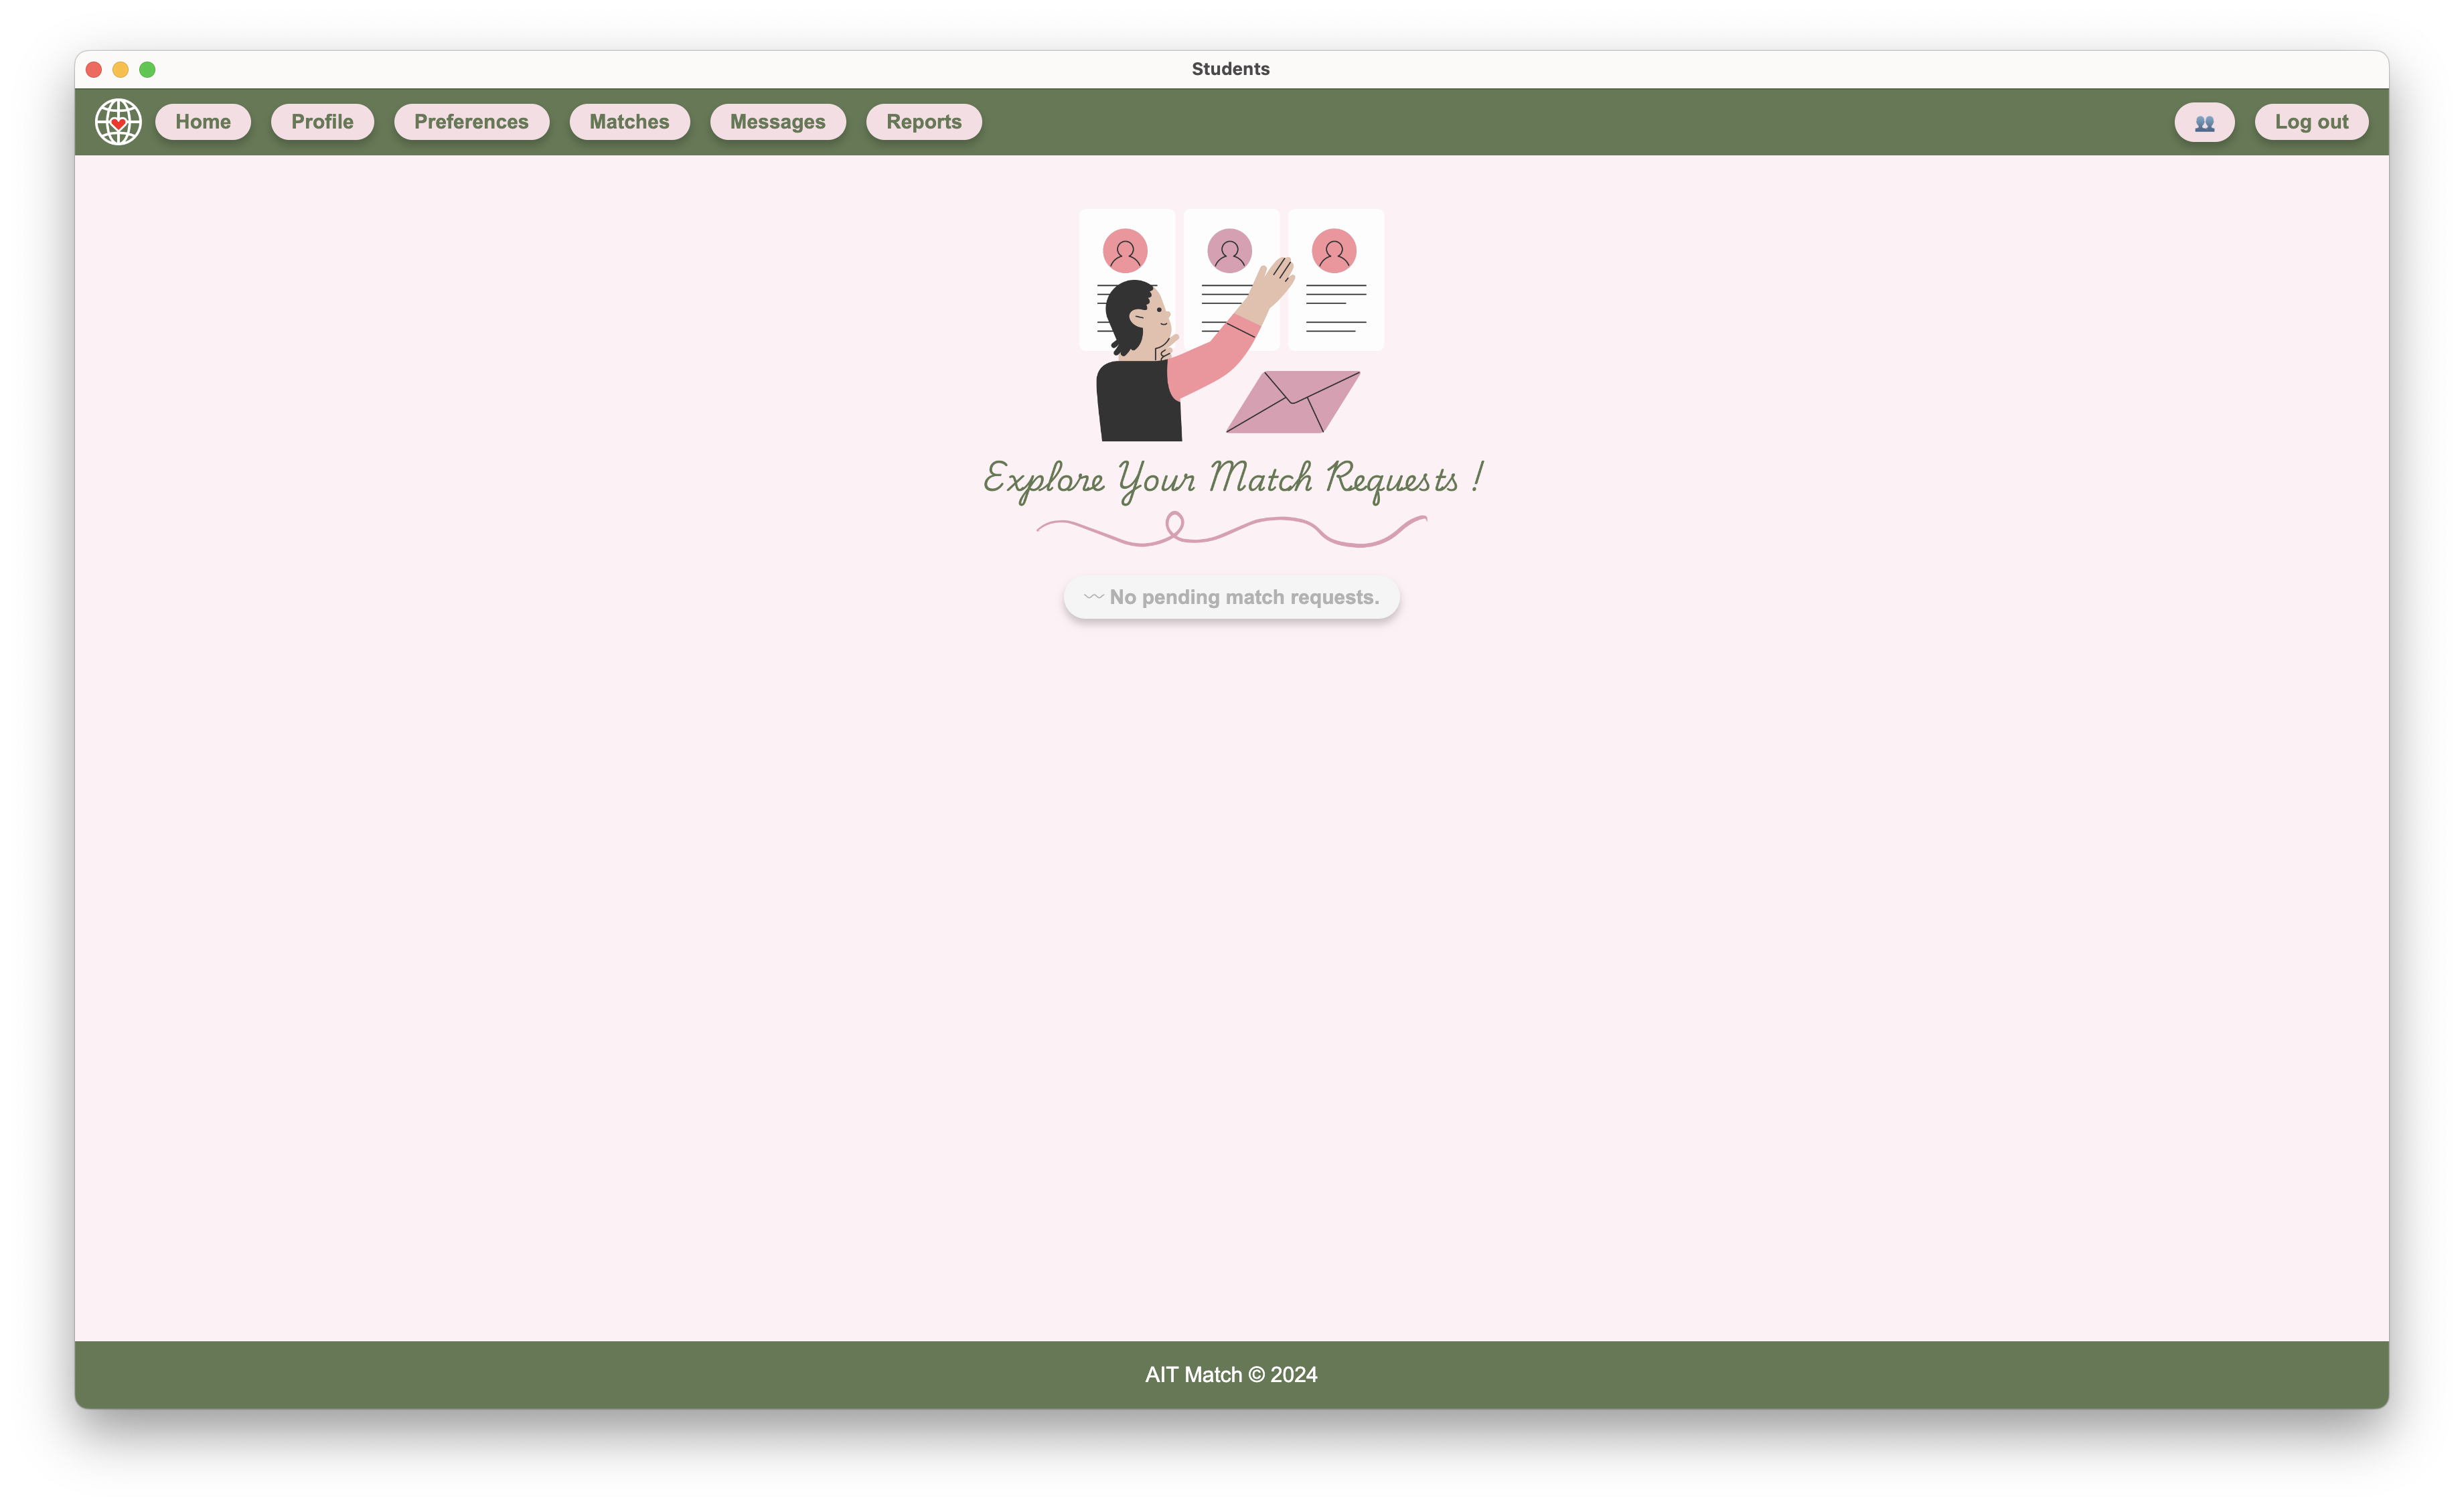
\includegraphics[width=5in]{figures/results/matches/no-match-request-page.png} 
                \caption{No Match Requests Page.}
                \label{fig:no-match-request-page}
            \end{figure}

        \subsection{Match: Match Requests Page}
        \begin{figure}[h]
                \centering
                \captionsetup{justification=centering, singlelinecheck=false, labelsep=space}
                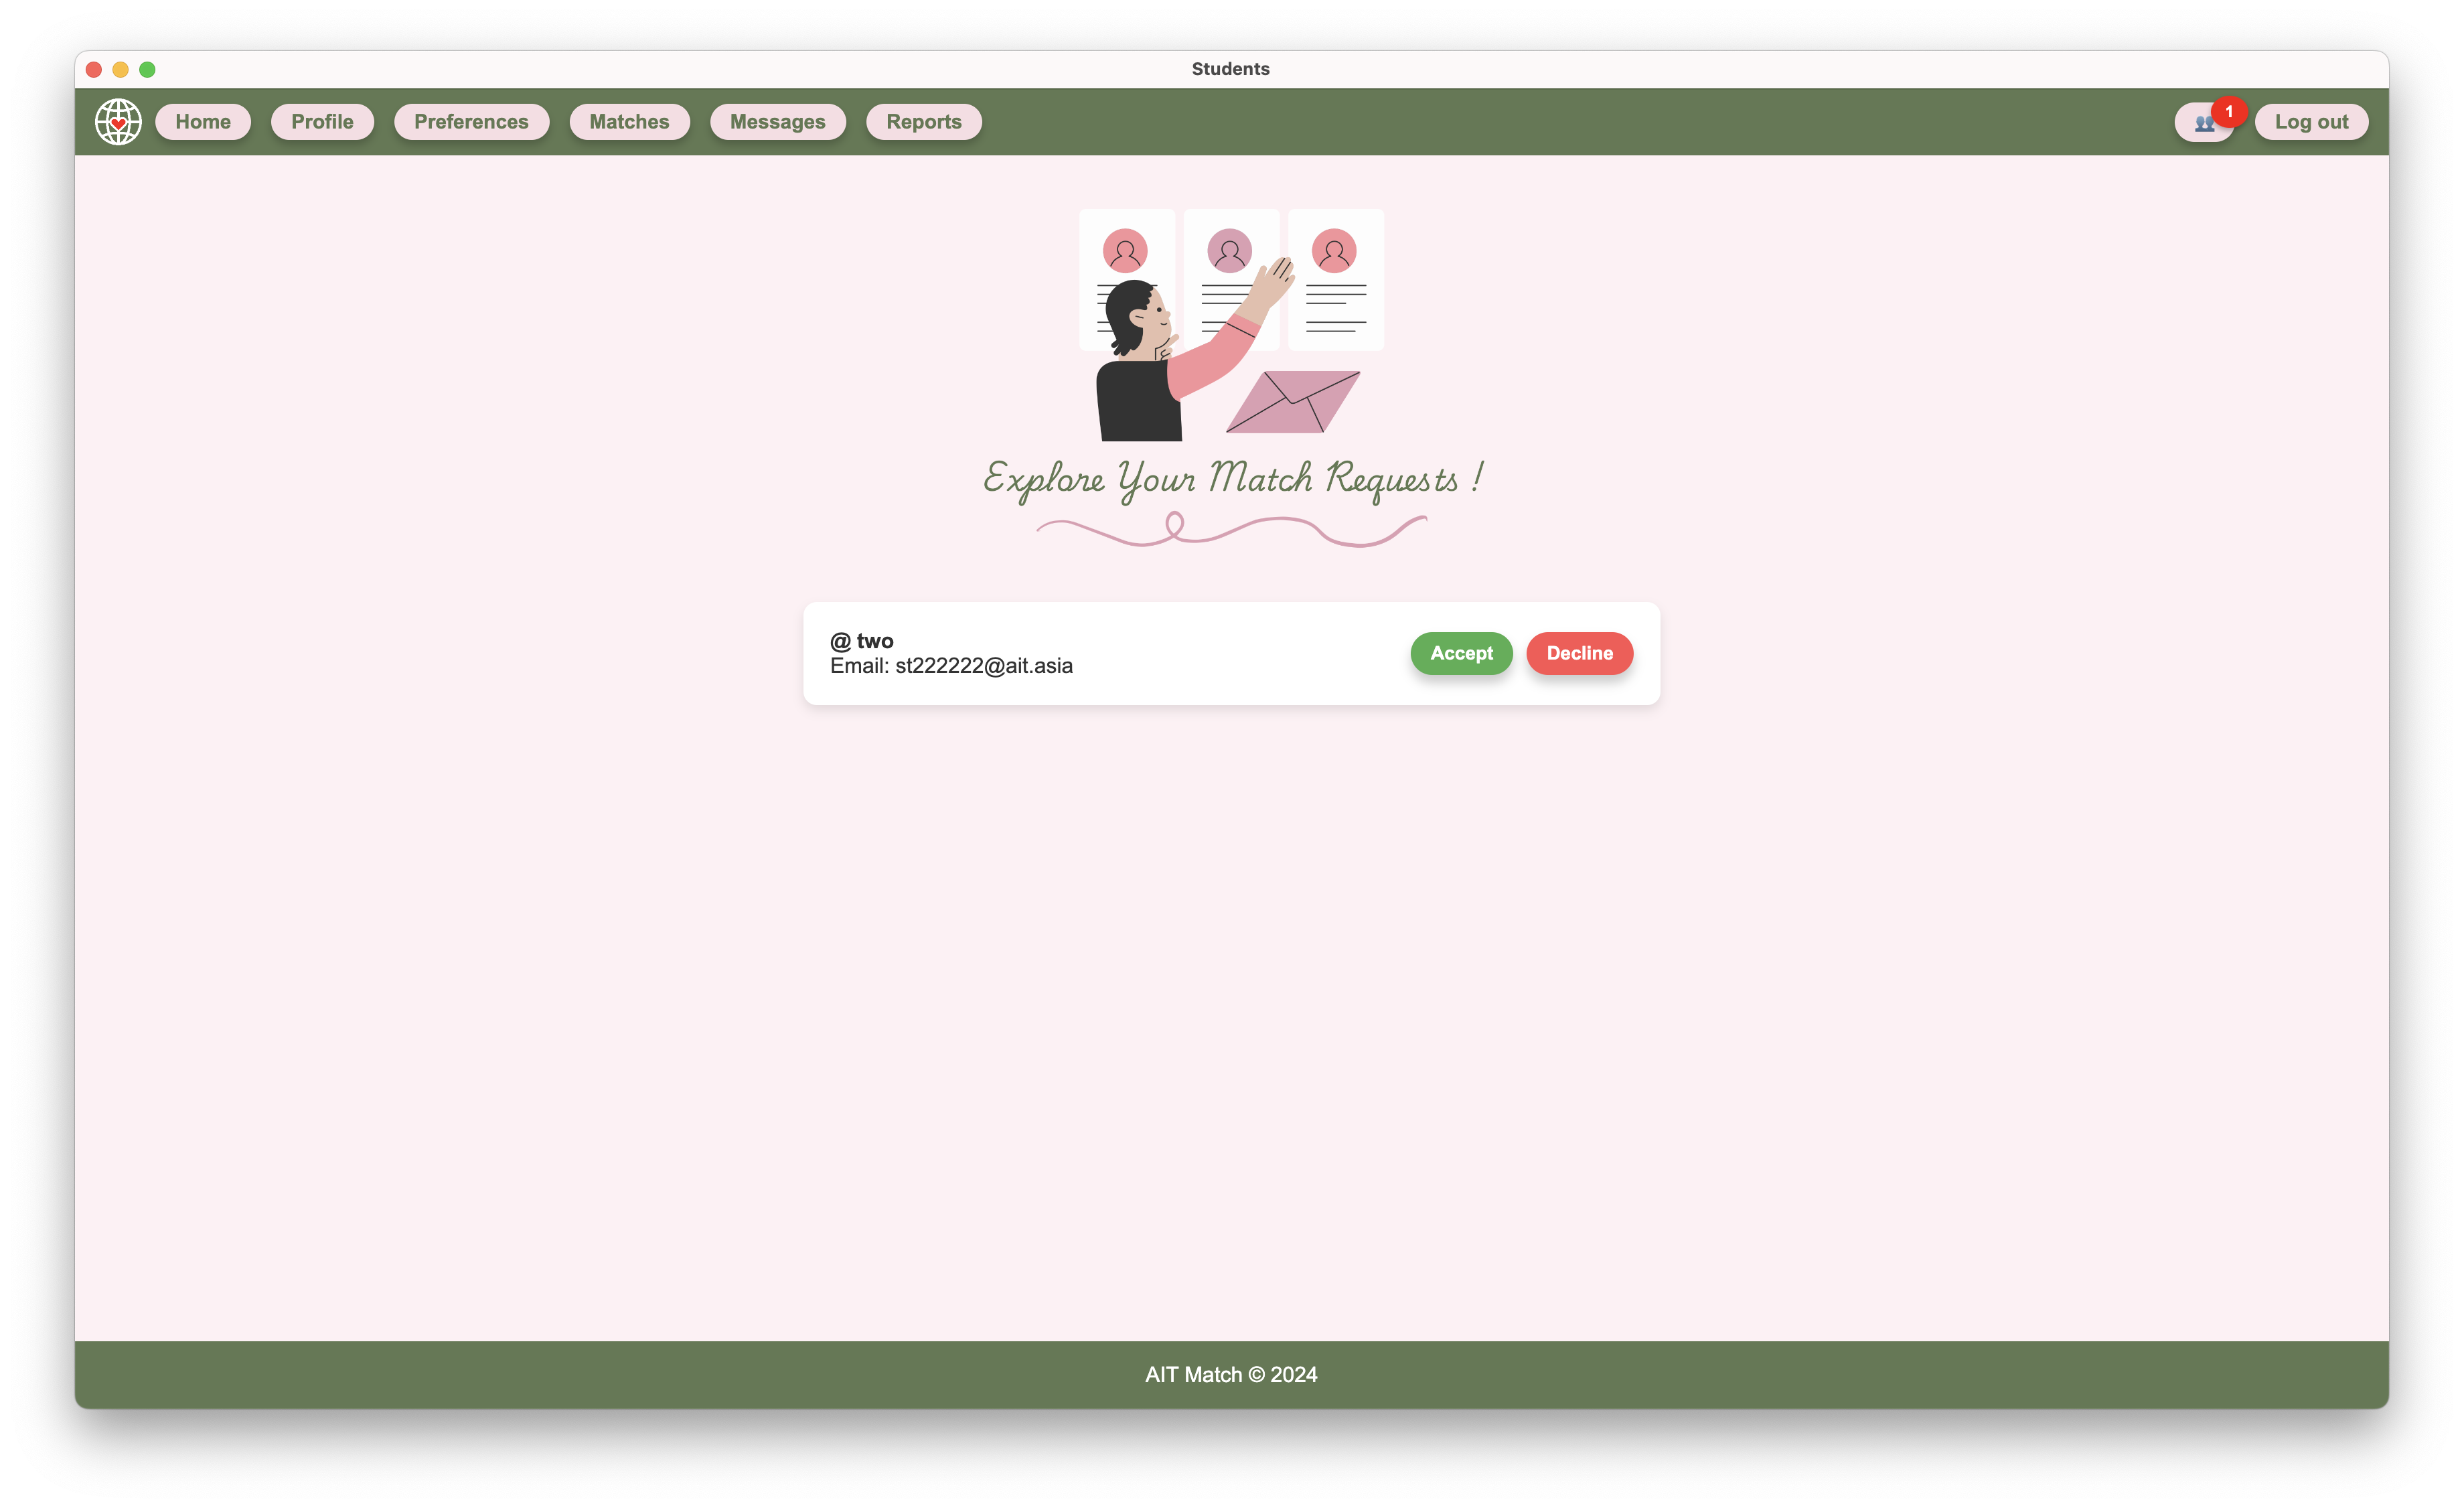
\includegraphics[width=5in]{figures/results/matches/match-request-page.png} 
                \caption{Match Requests Page.}
                \label{fig:match-request-page}
            \end{figure}

        \newpage
        \subsection{Match: No Matched Profiles Page}
        \begin{figure}[h]
                \centering
                \captionsetup{justification=centering, singlelinecheck=false, labelsep=space}
                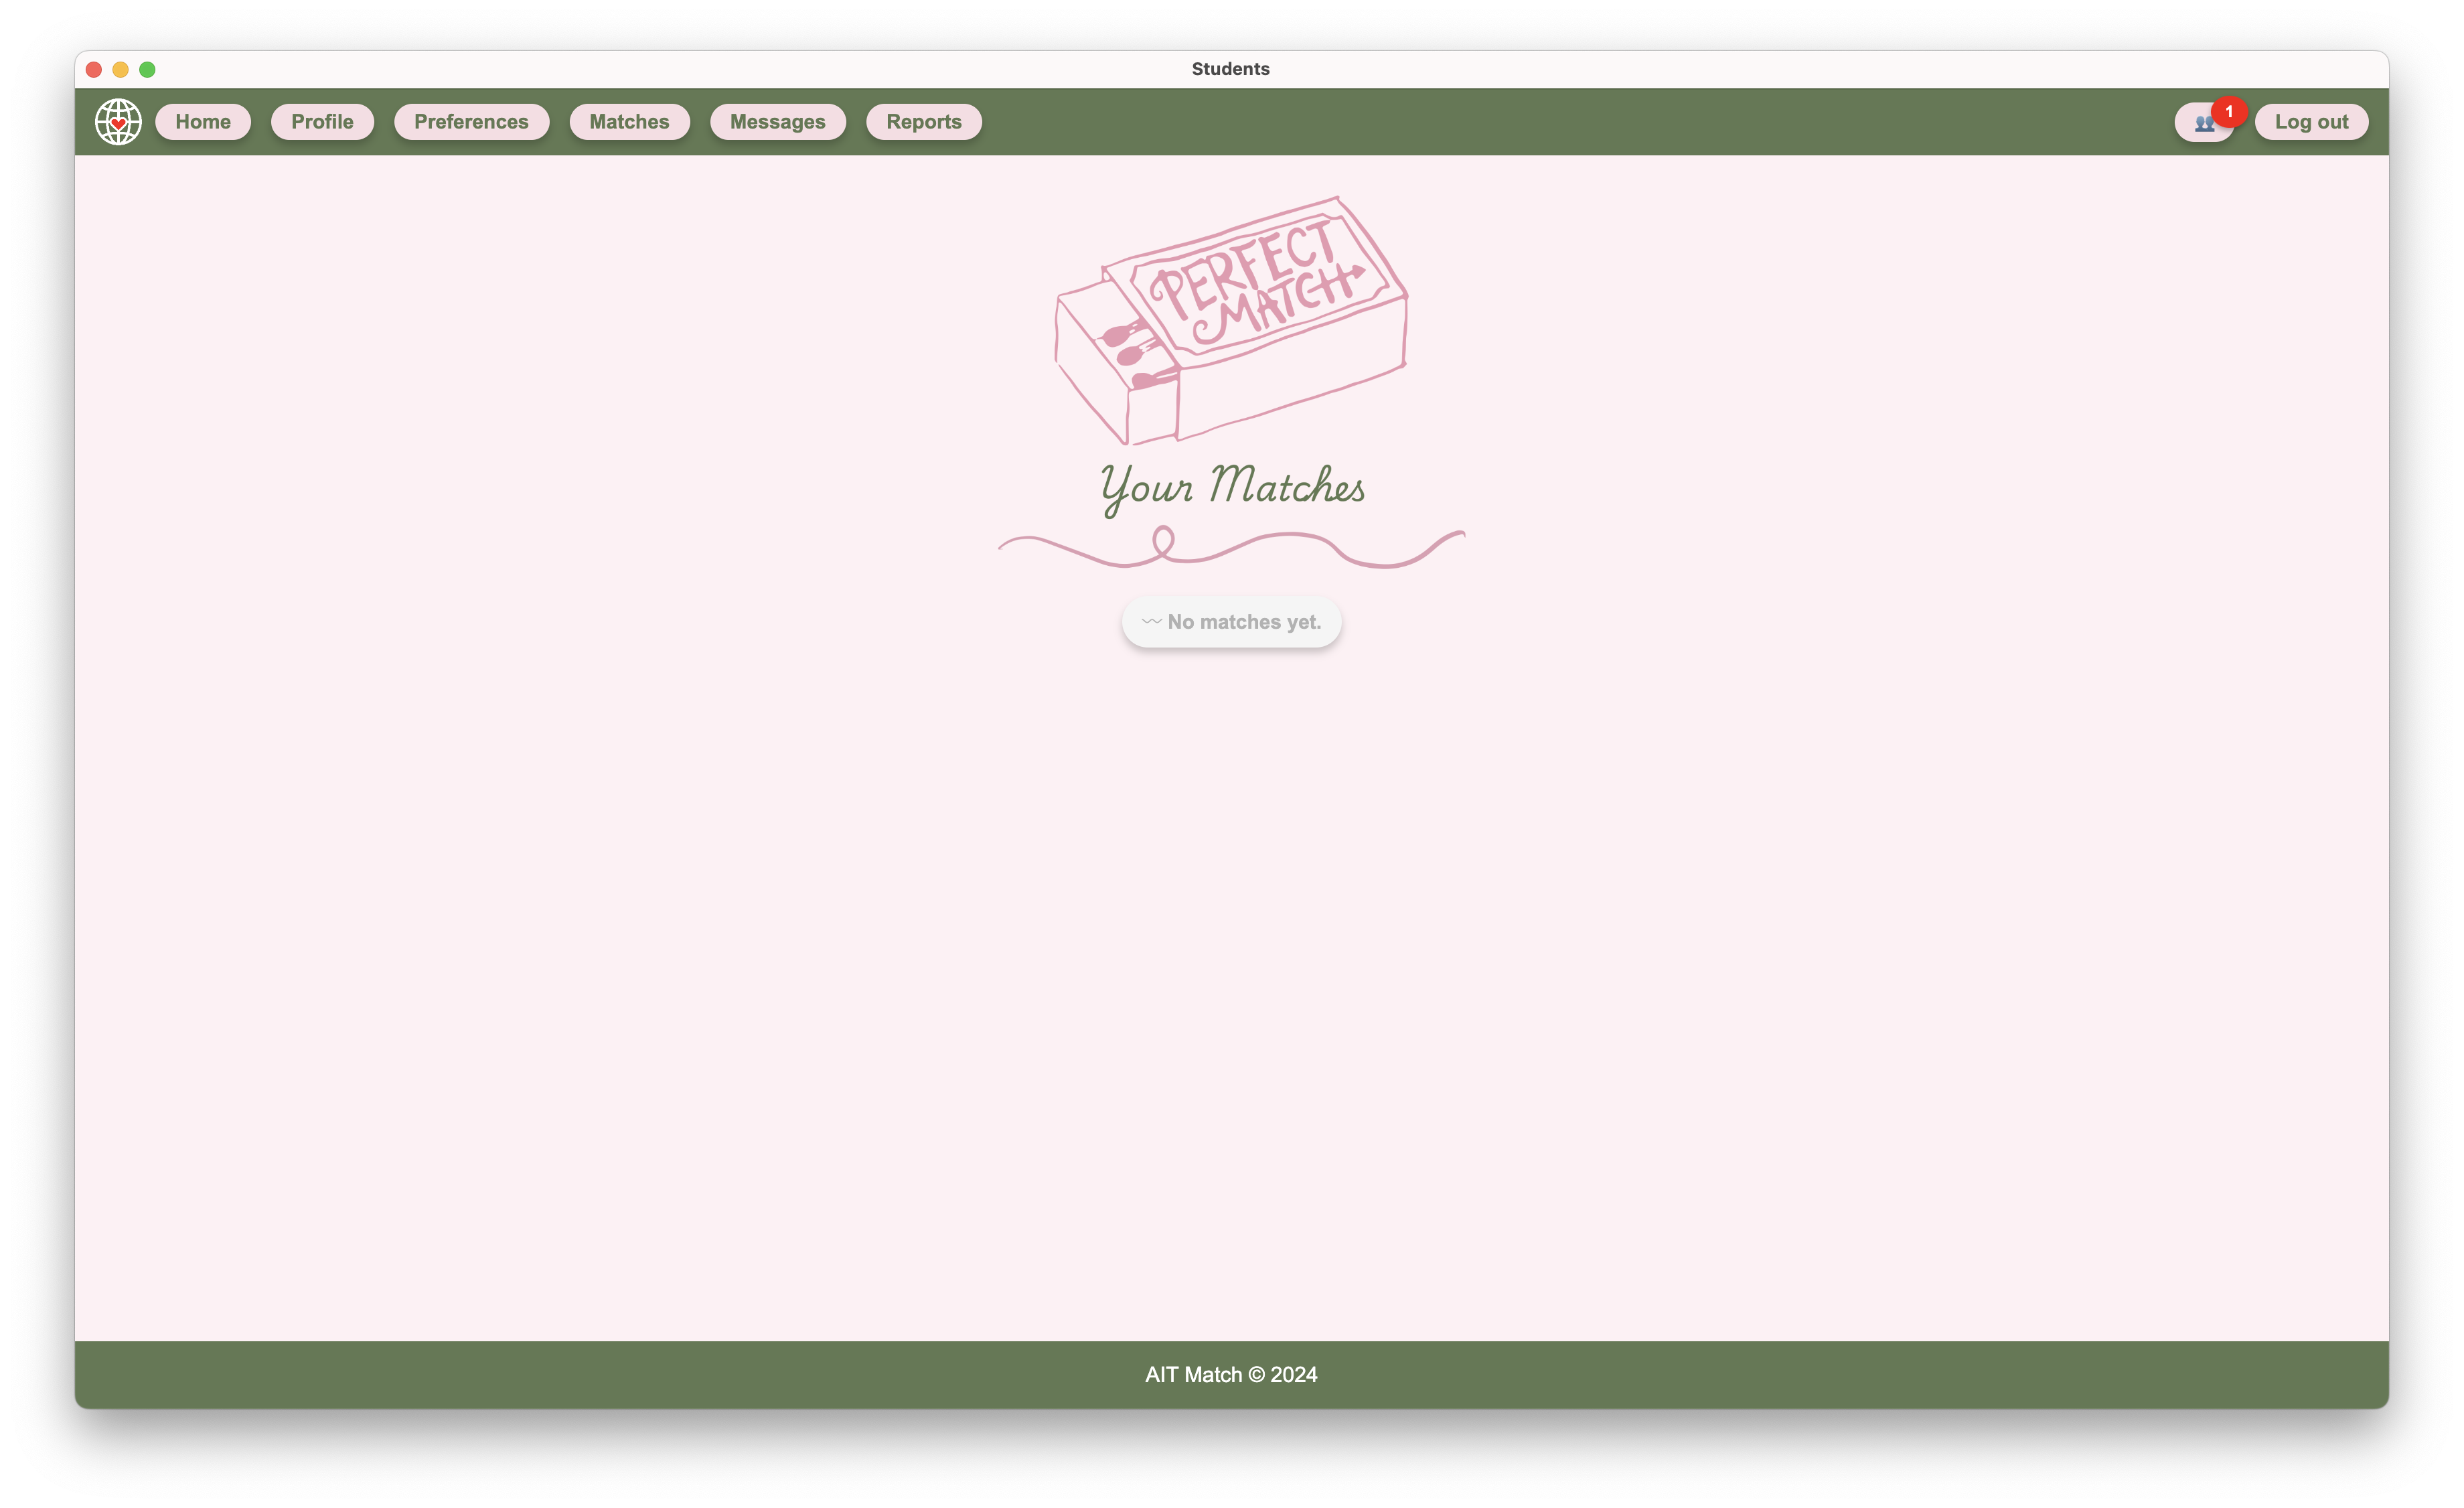
\includegraphics[width=5in]{figures/results/matches/no-matched-profile-page.png} 
                \caption{No Matched Profiles Page.}
                \label{fig:no-matched-profile-page}
            \end{figure}

        \subsection{Match: Matched Profiles Page}
        \begin{figure}[h]
                \centering
                \captionsetup{justification=centering, singlelinecheck=false, labelsep=space}
                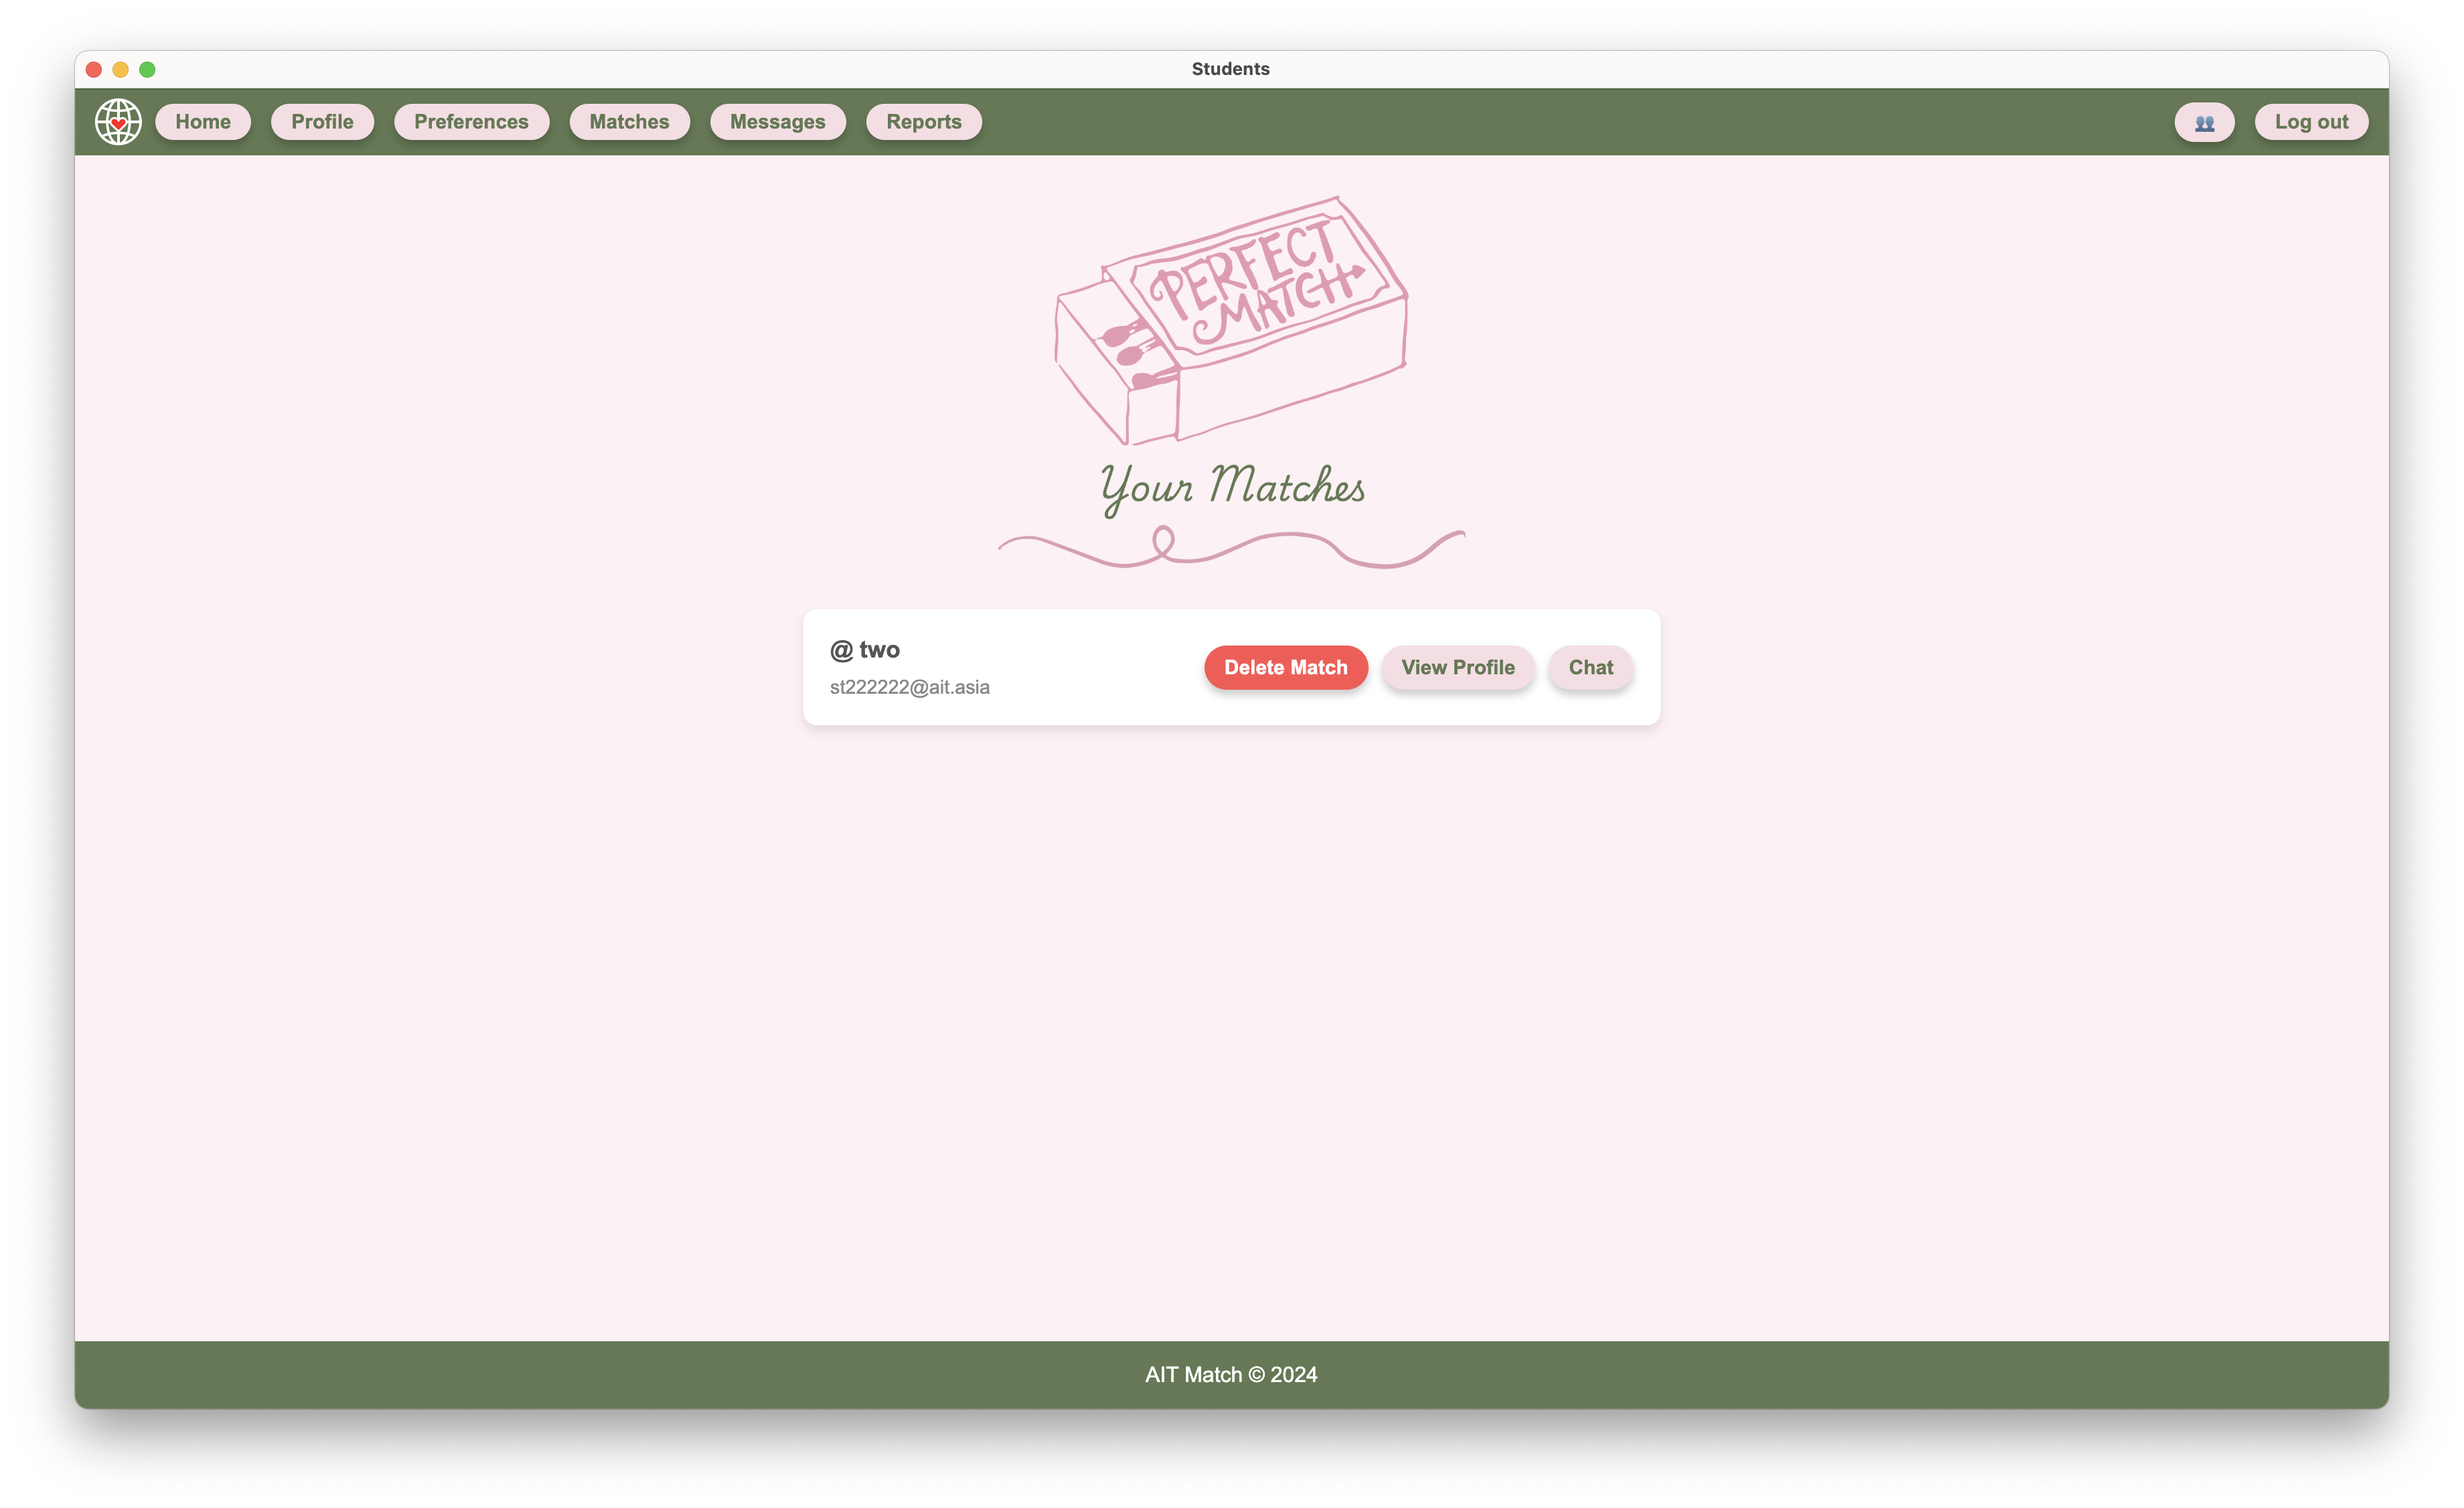
\includegraphics[width=5in]{figures/results/matches/matched-profile-page.png} 
                \caption{Matched Profiles Page.}
                \label{fig:matched-profile-page}
            \end{figure}
% ------------------------------------------------- %
        \newpage
        \subsection{Conversation: No Conversations Page}
        \begin{figure}[h]
                \centering
                \captionsetup{justification=centering, singlelinecheck=false, labelsep=space}
                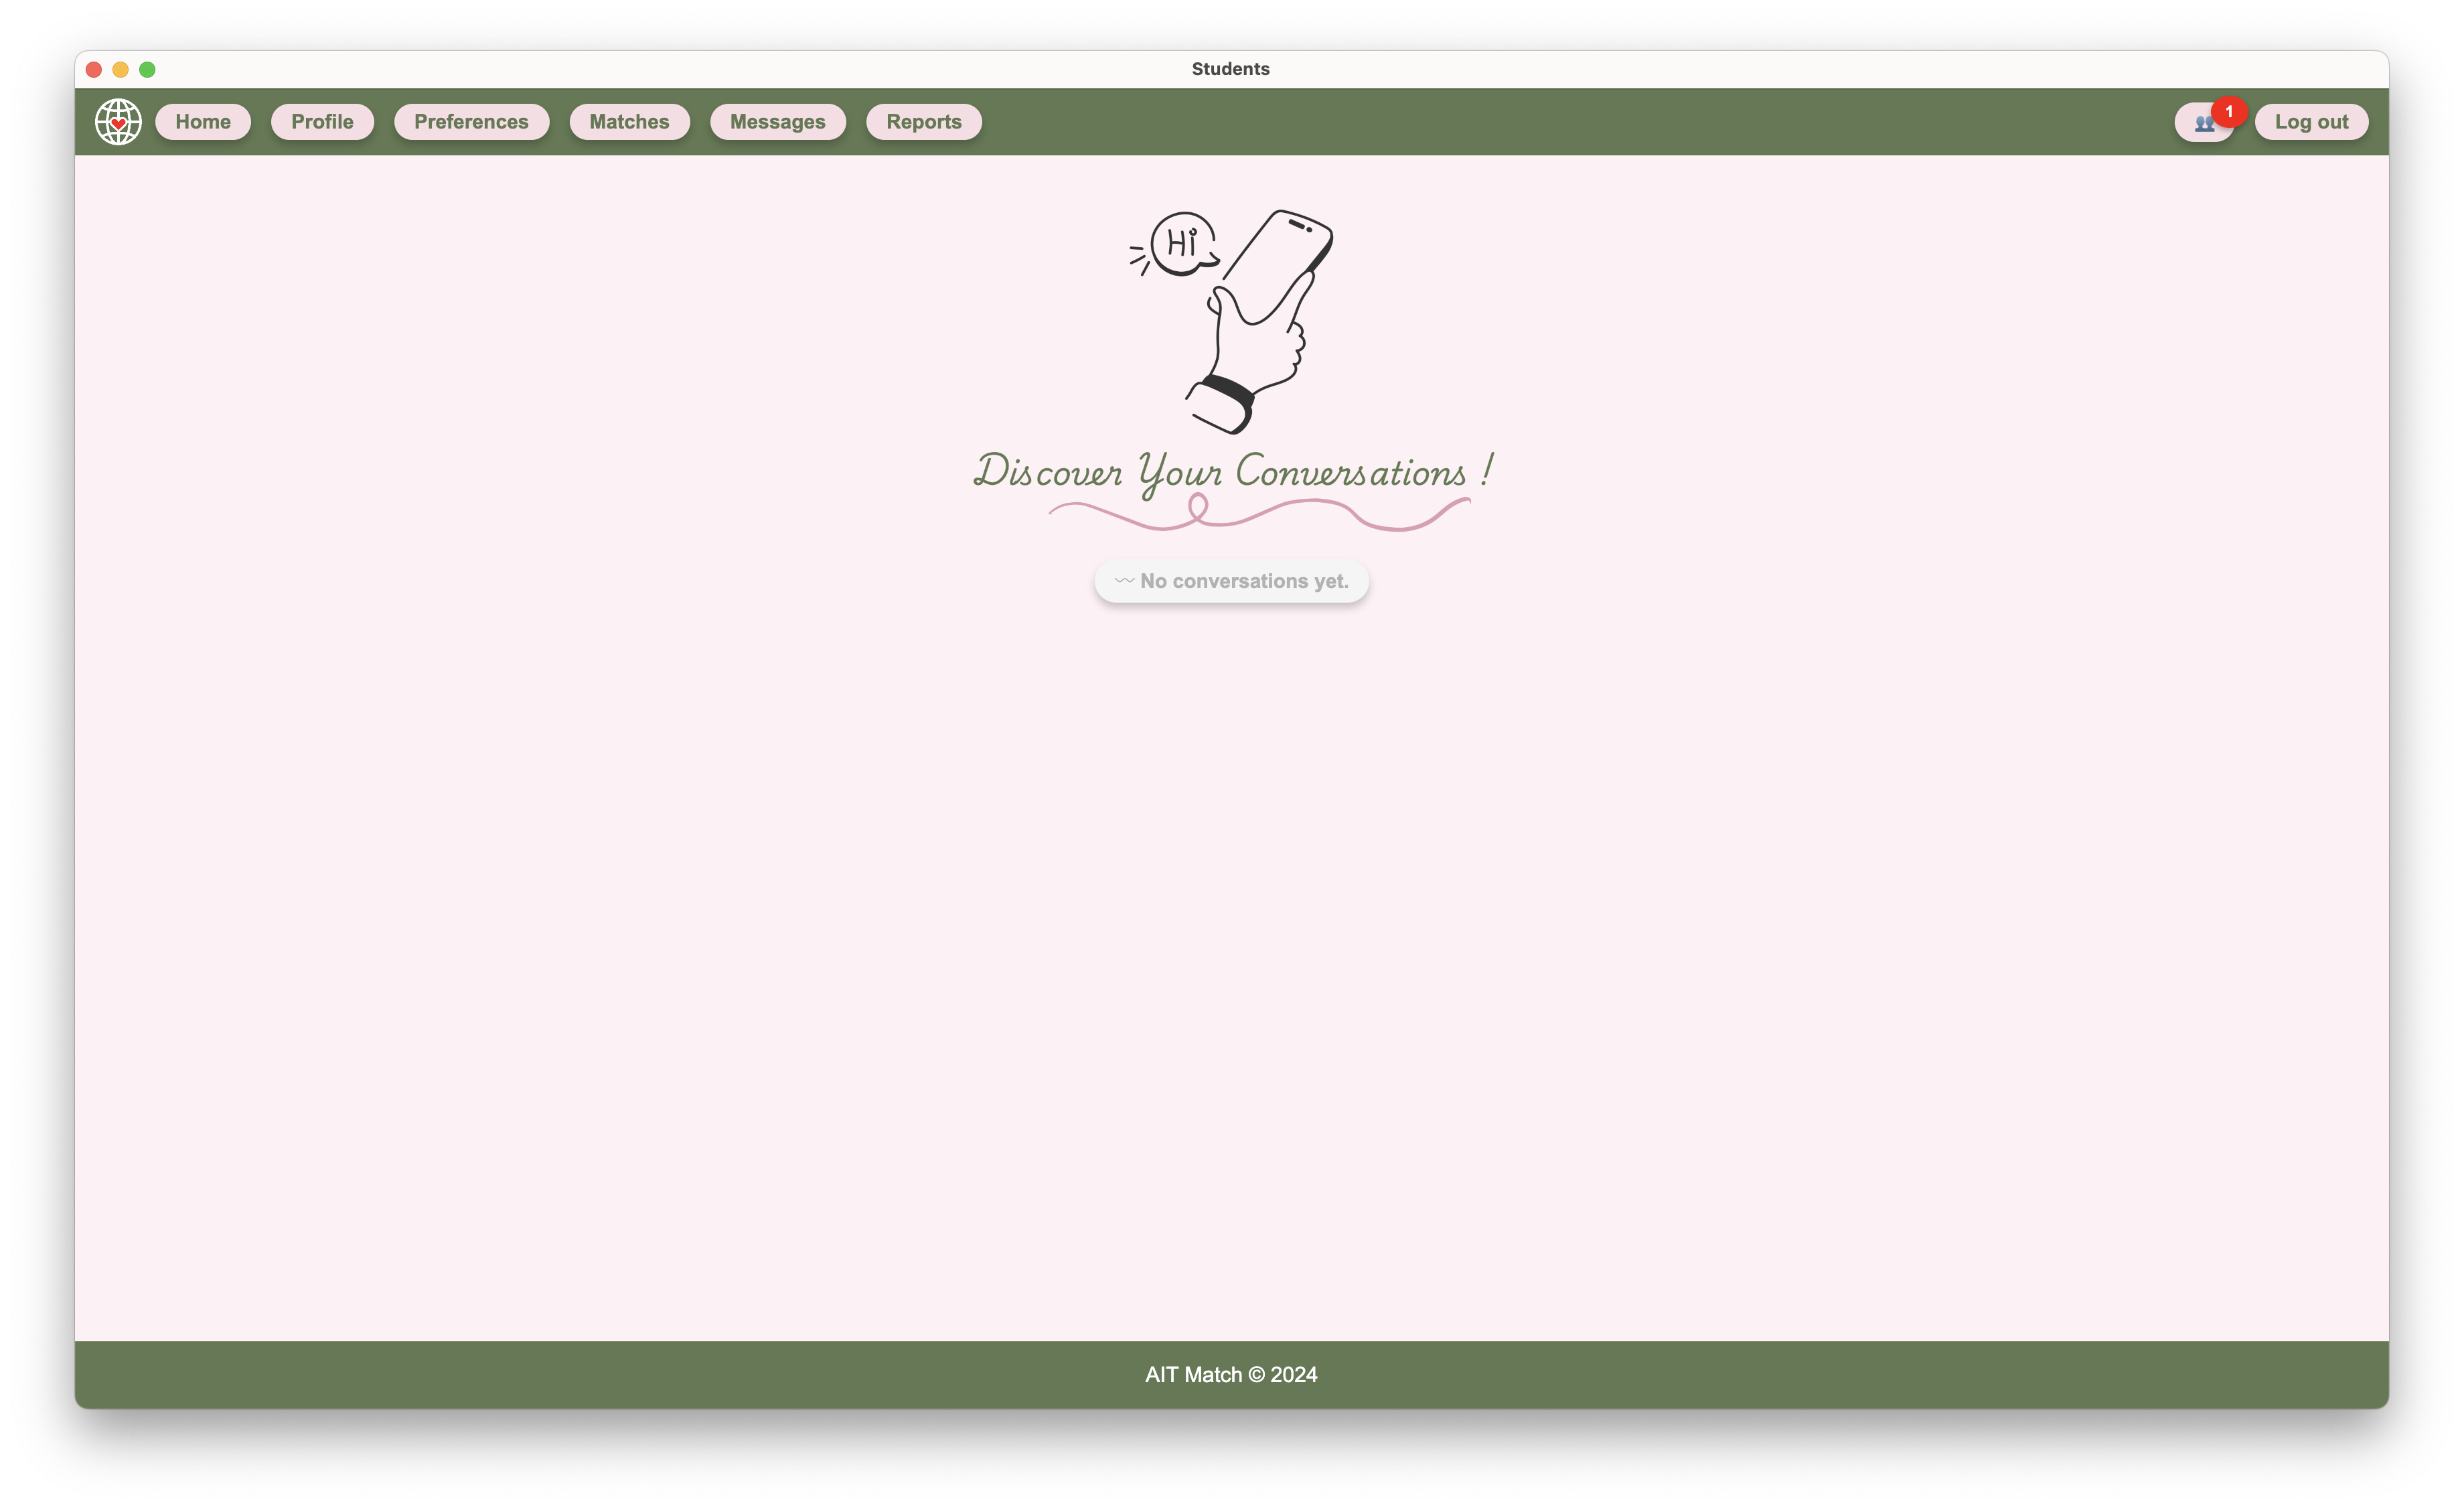
\includegraphics[width=5in]{figures/results/conversations/no-conversation-page.png} 
                \caption{No Conversations Page.}
                \label{fig:no-conversation-page.png}
            \end{figure}

        \subsection{Conversation: Conversations Page}
        \begin{figure}[h]
                \centering
                \captionsetup{justification=centering, singlelinecheck=false, labelsep=space}
                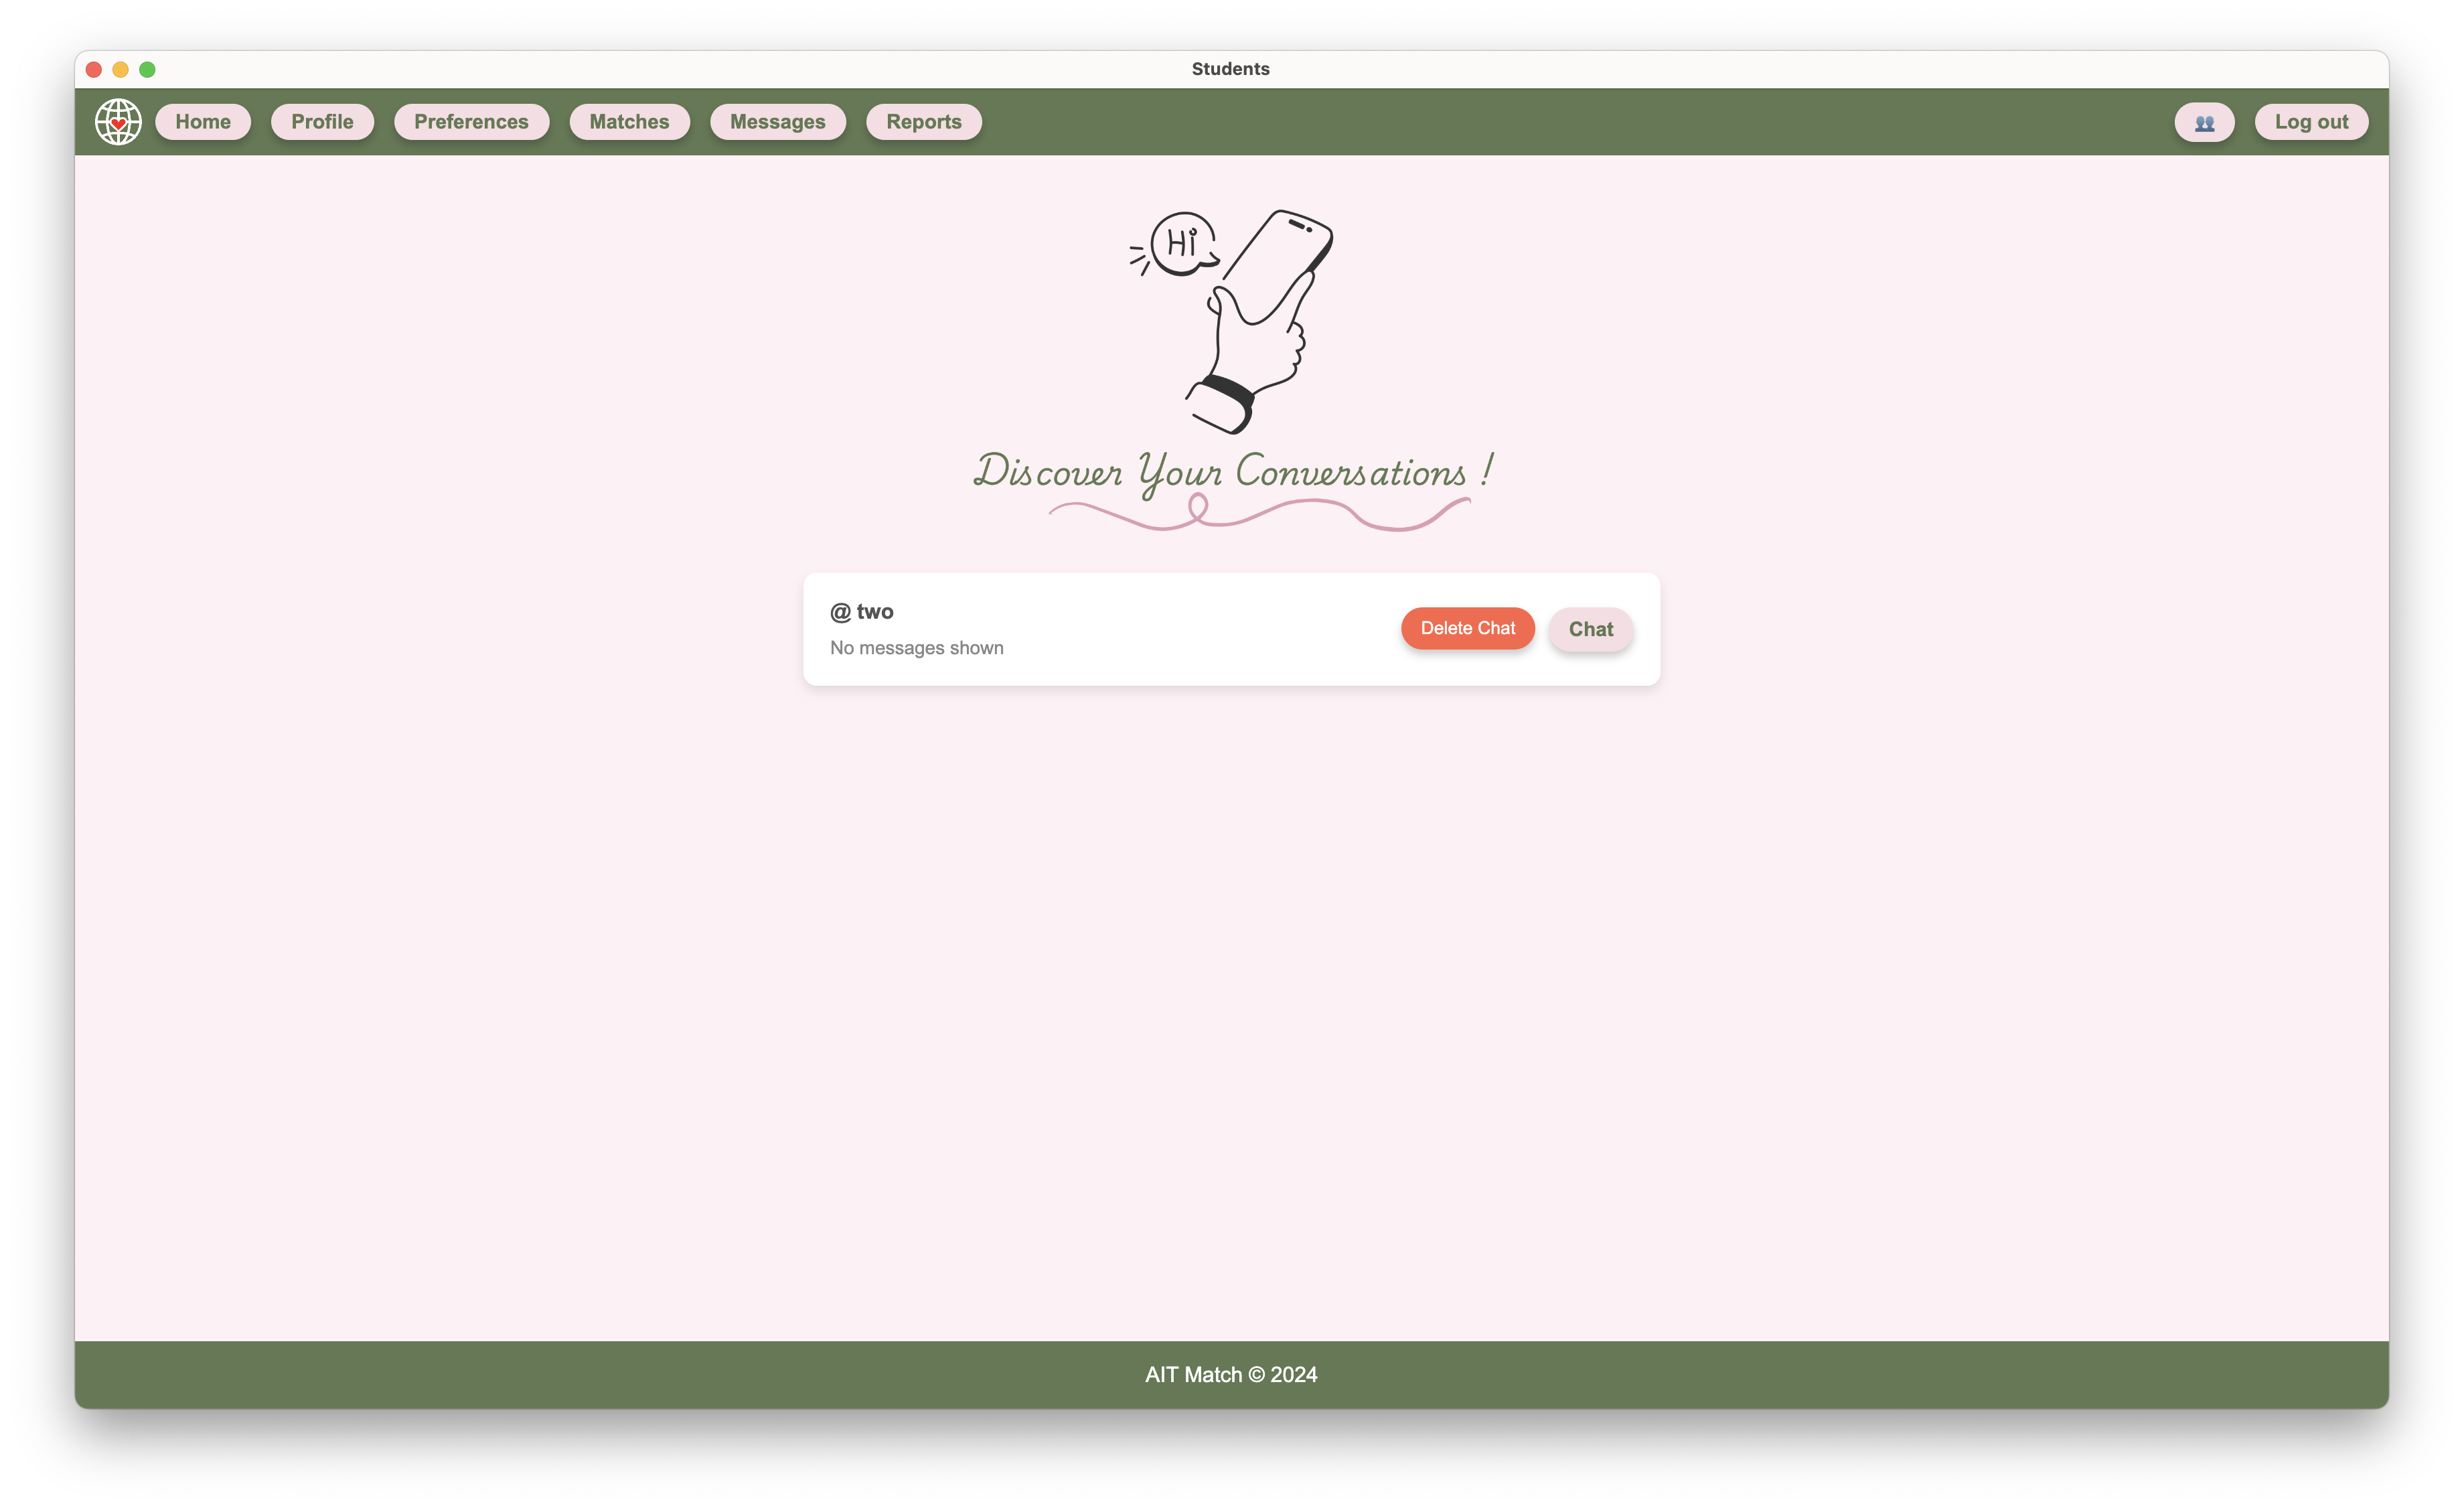
\includegraphics[width=5in]{figures/results/conversations/conversation-page.png} 
                \caption{Conversations Page.}
                \label{fig:conversation-page.png}
            \end{figure}
% ------------------------------------------------- %
        \newpage
        \subsection{Chat: Chat Room Page}
        \begin{figure}[h]
                \centering
                \captionsetup{justification=centering, singlelinecheck=false, labelsep=space}
                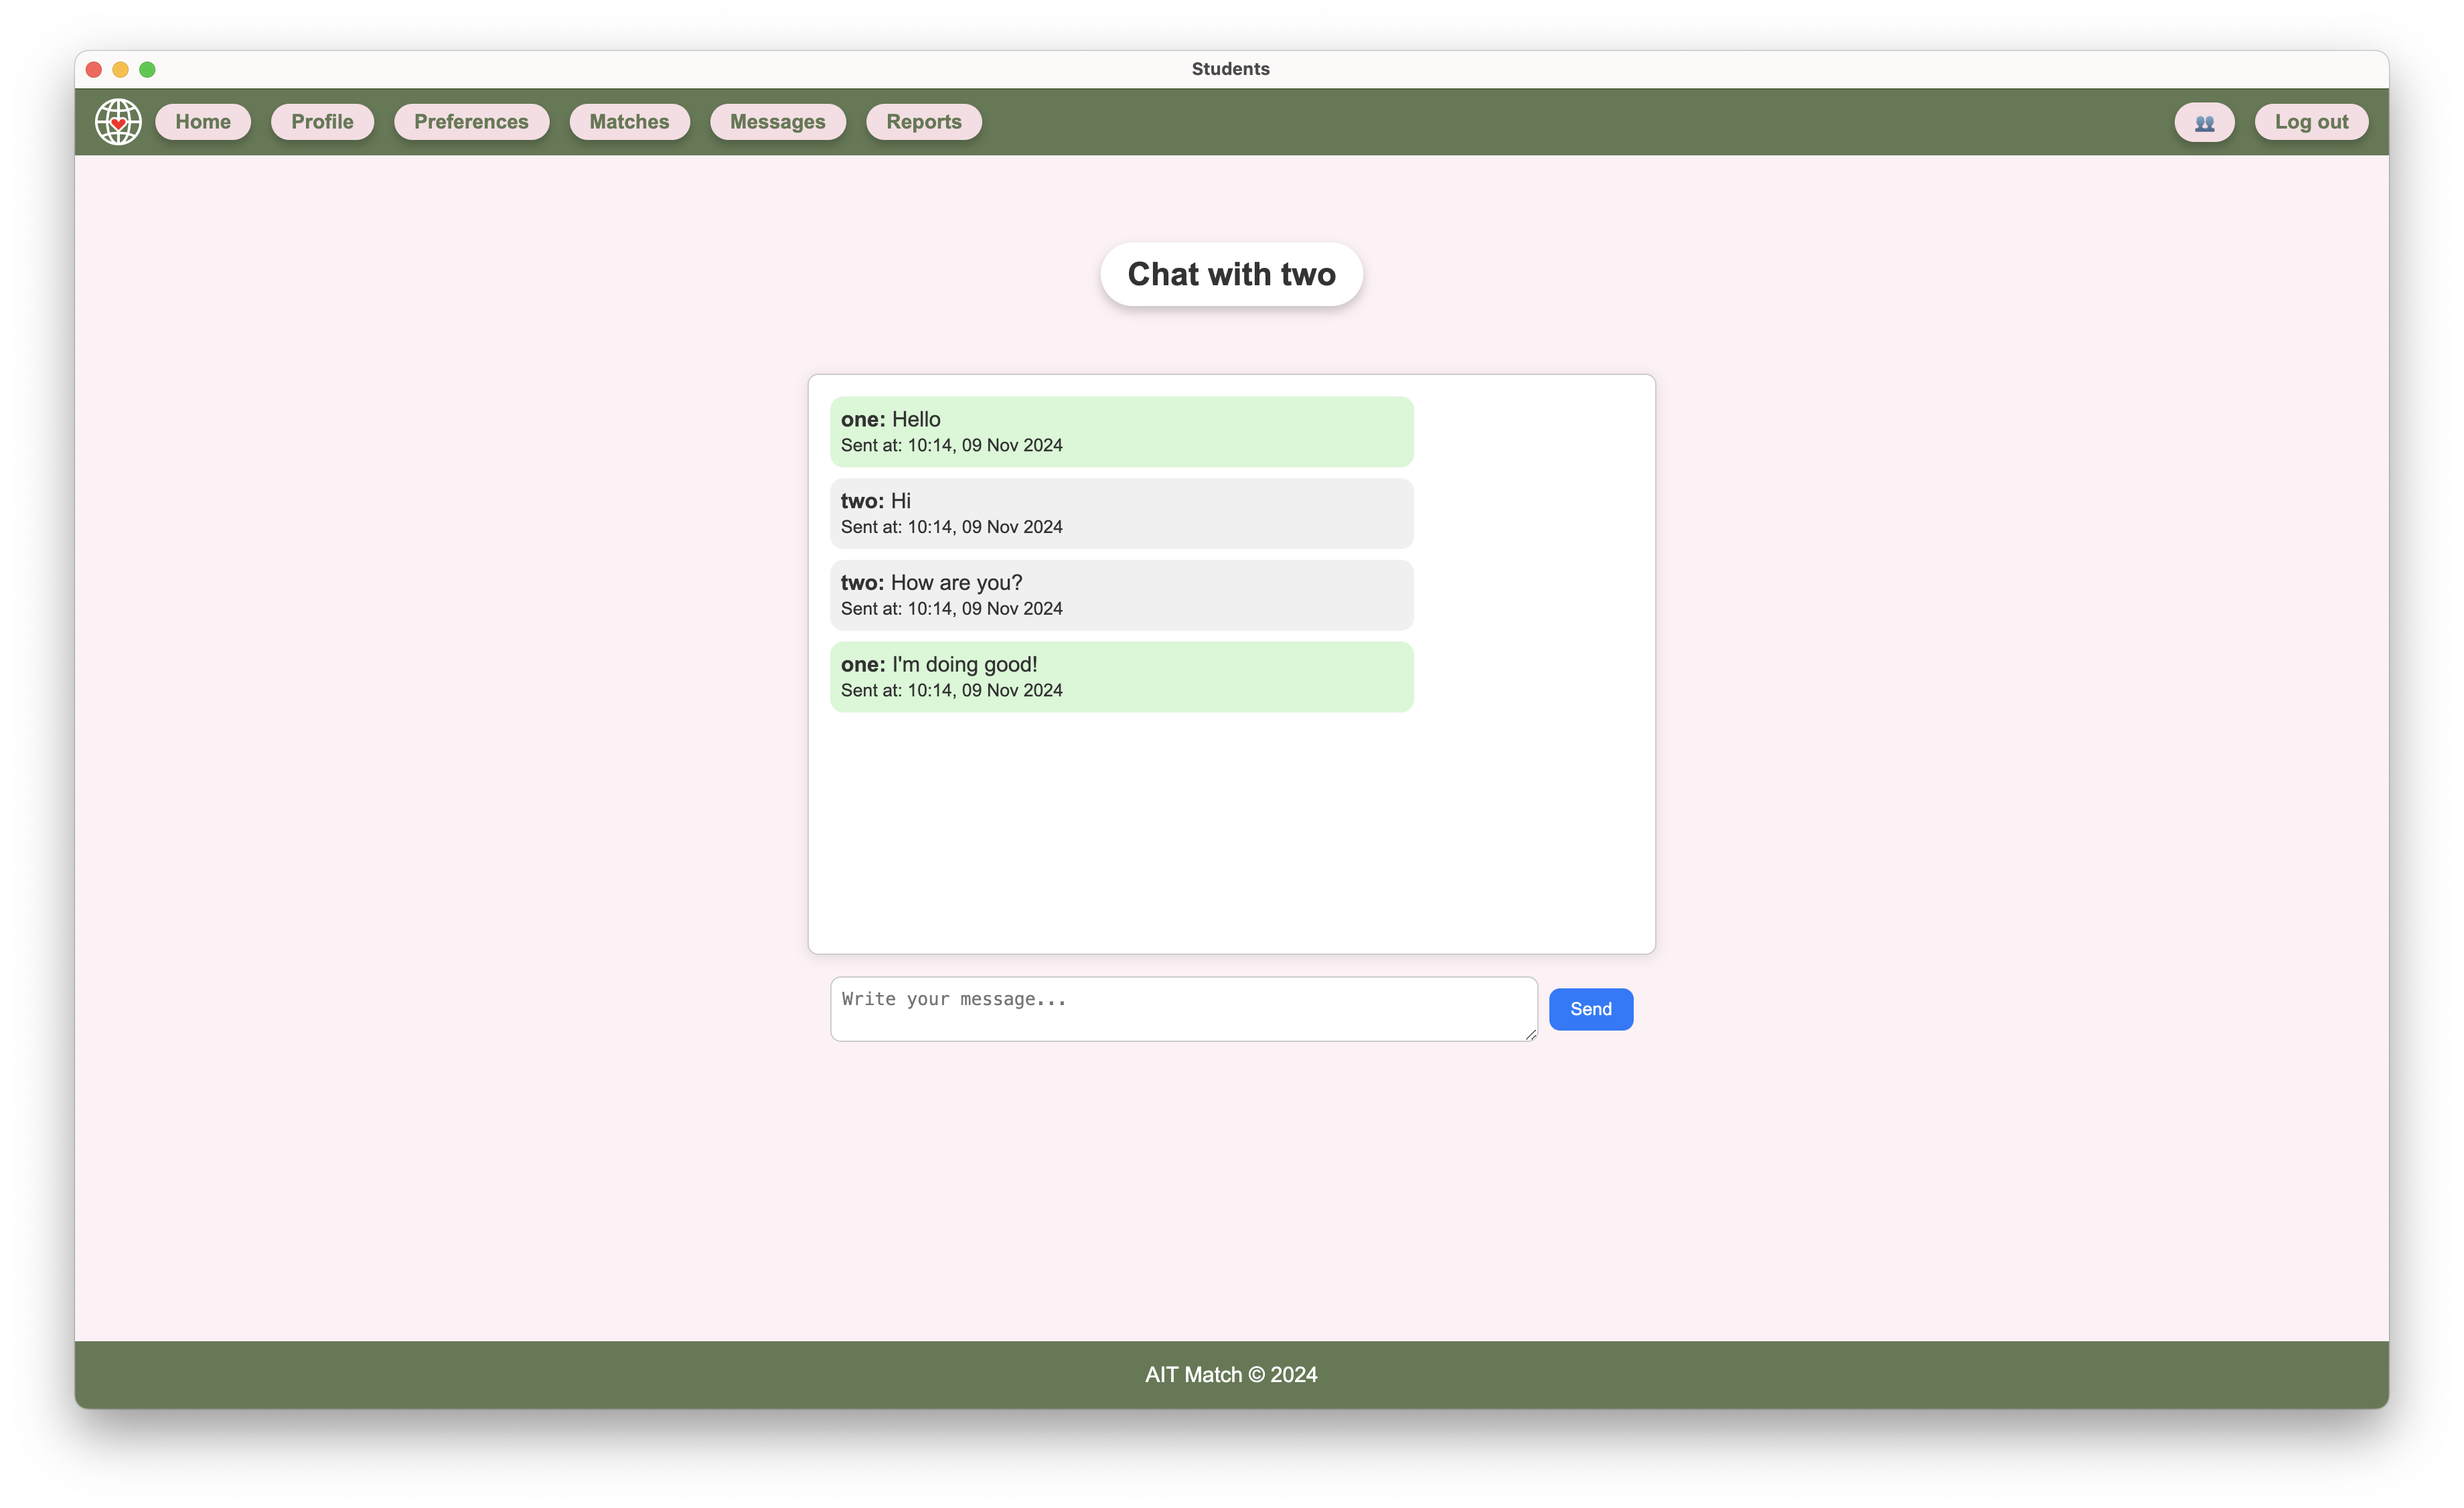
\includegraphics[width=5in]{figures/results/chat/chat-room-page.png} 
                \caption{Chat Room Page.}
                \label{fig:no-conversation-page.png}
            \end{figure}
% ------------------------------------------------- %
        \newpage
        \subsection{Report: Reported Profile Page}
        \begin{figure}[h]
                \centering
                \captionsetup{justification=centering, singlelinecheck=false, labelsep=space}
                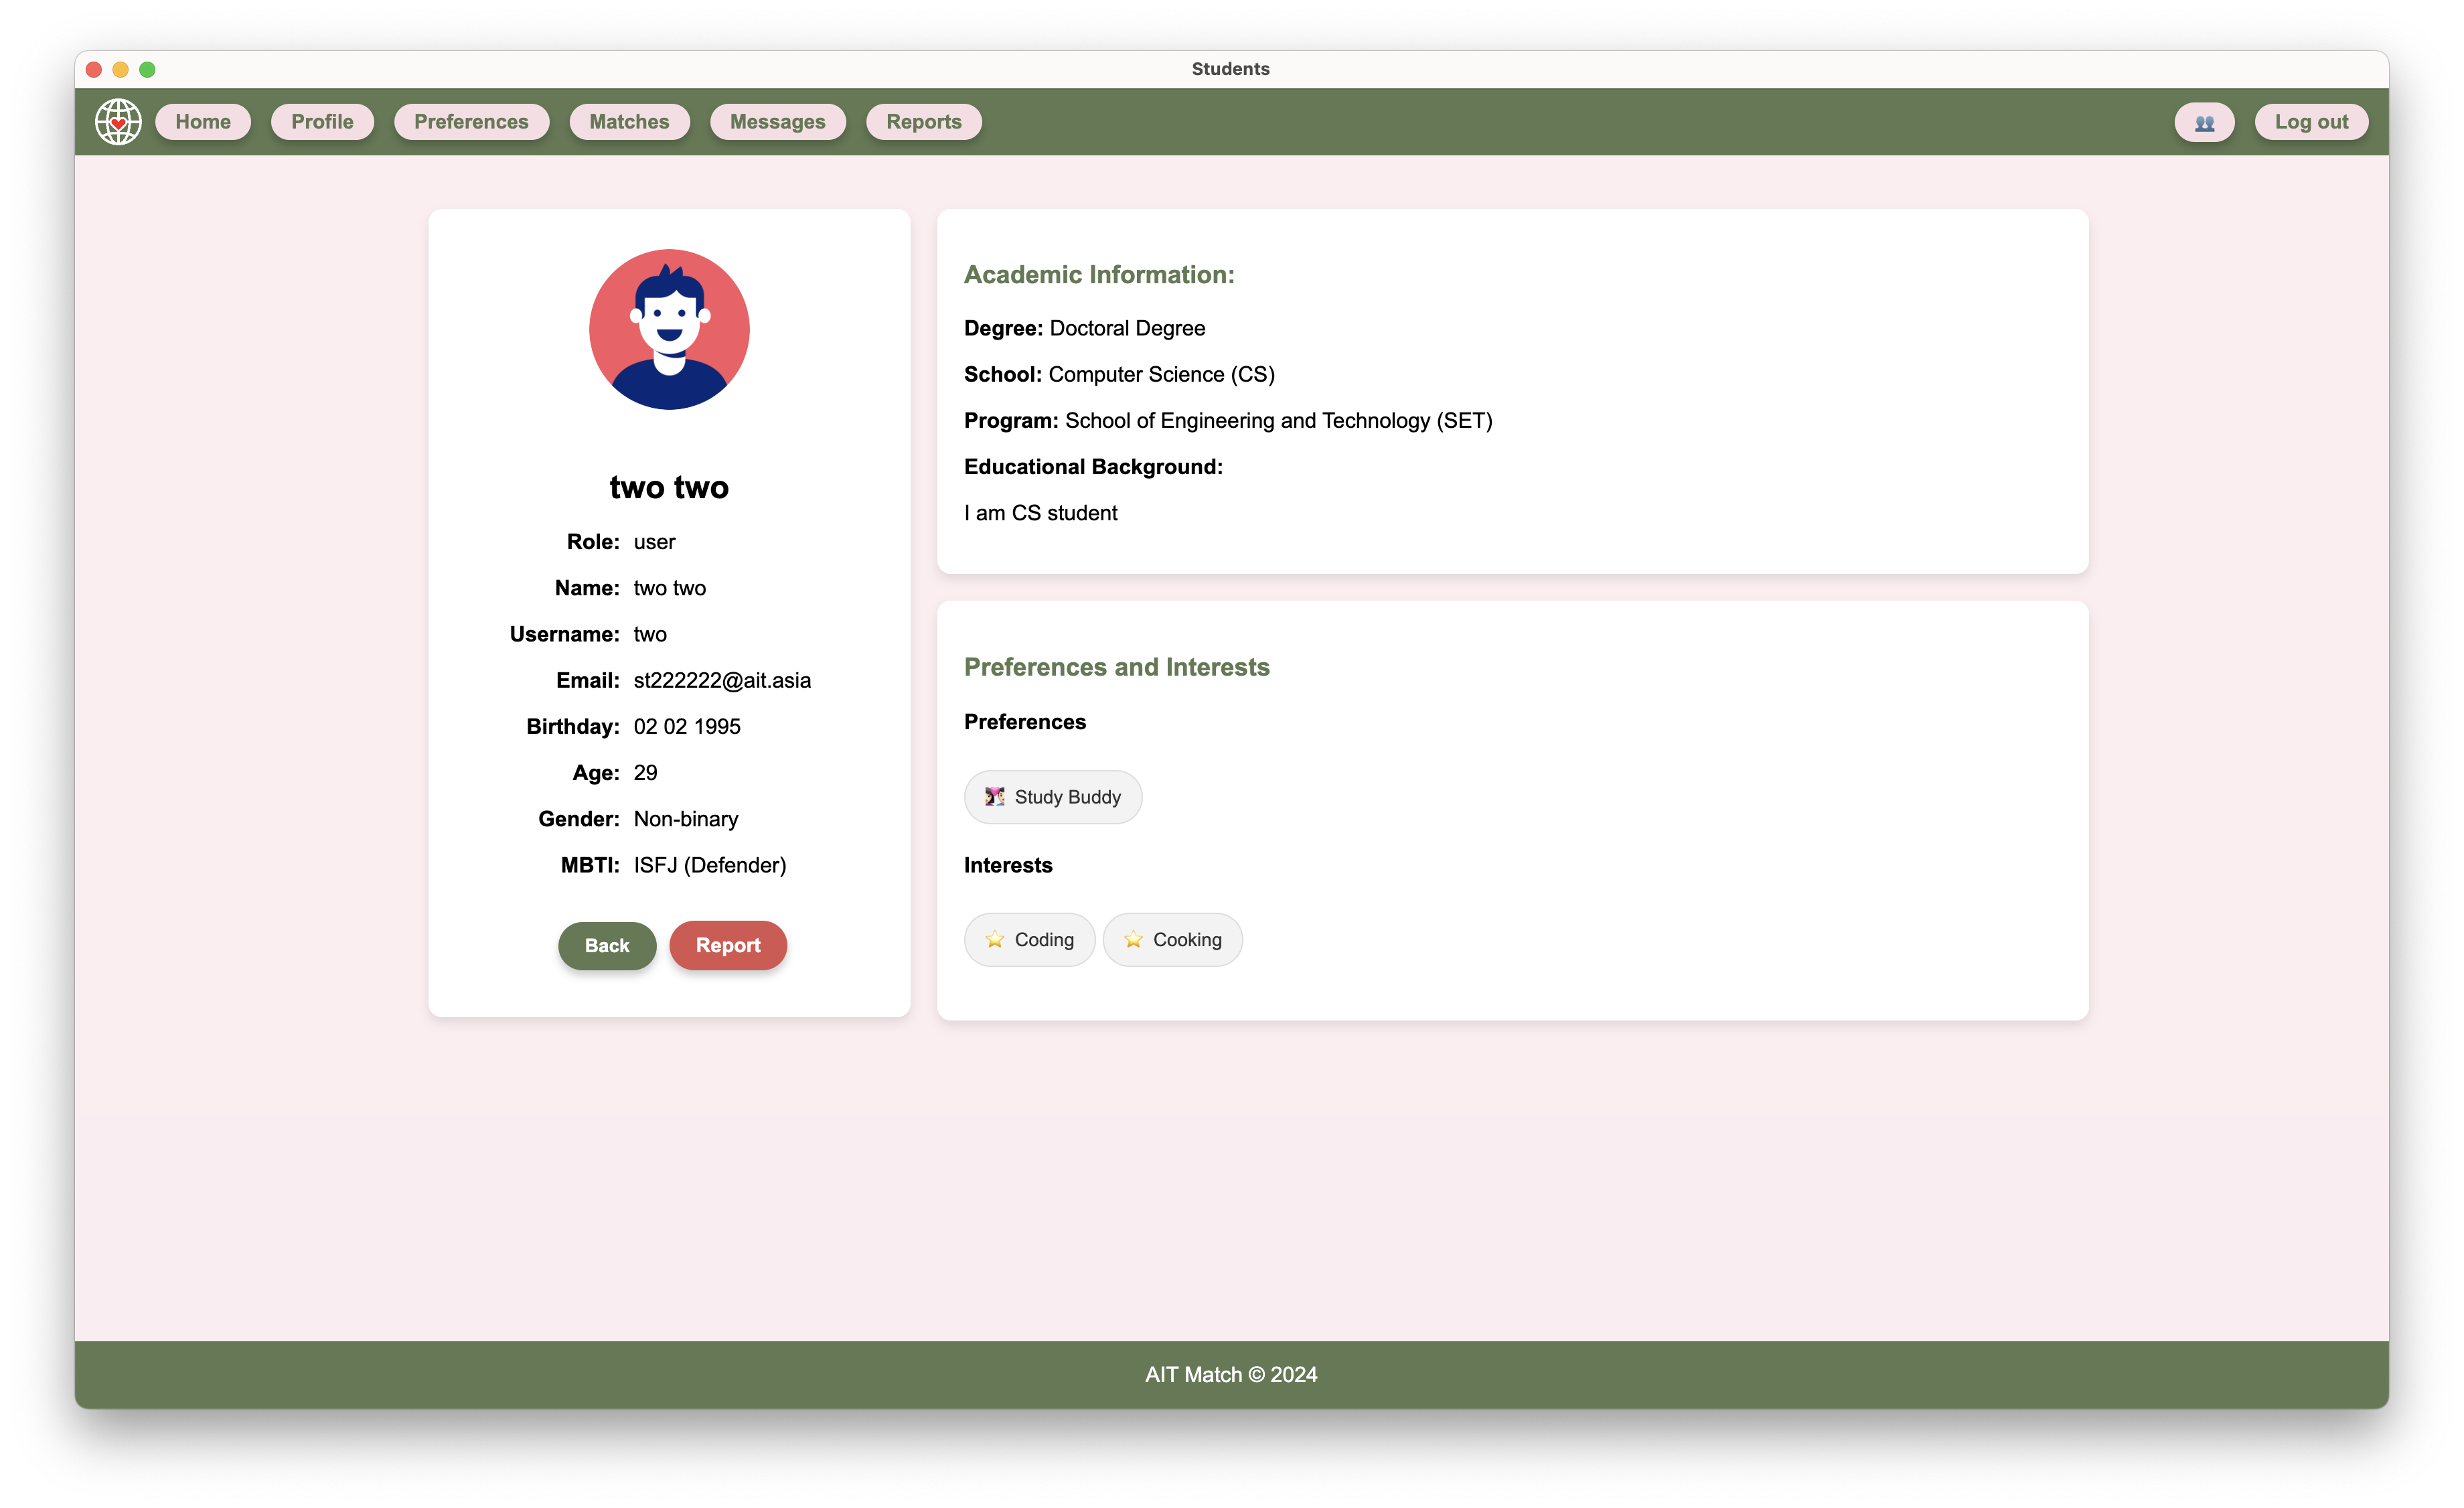
\includegraphics[width=5in]{figures/results/reports/reported-profile-page.png} 
                \caption{Reported Profile Page.}
                \label{fig:reported-profile-page}
            \end{figure}

        \subsection{Report: New Report Page}
        \begin{figure}[h]
                \centering
                \captionsetup{justification=centering, singlelinecheck=false, labelsep=space}
                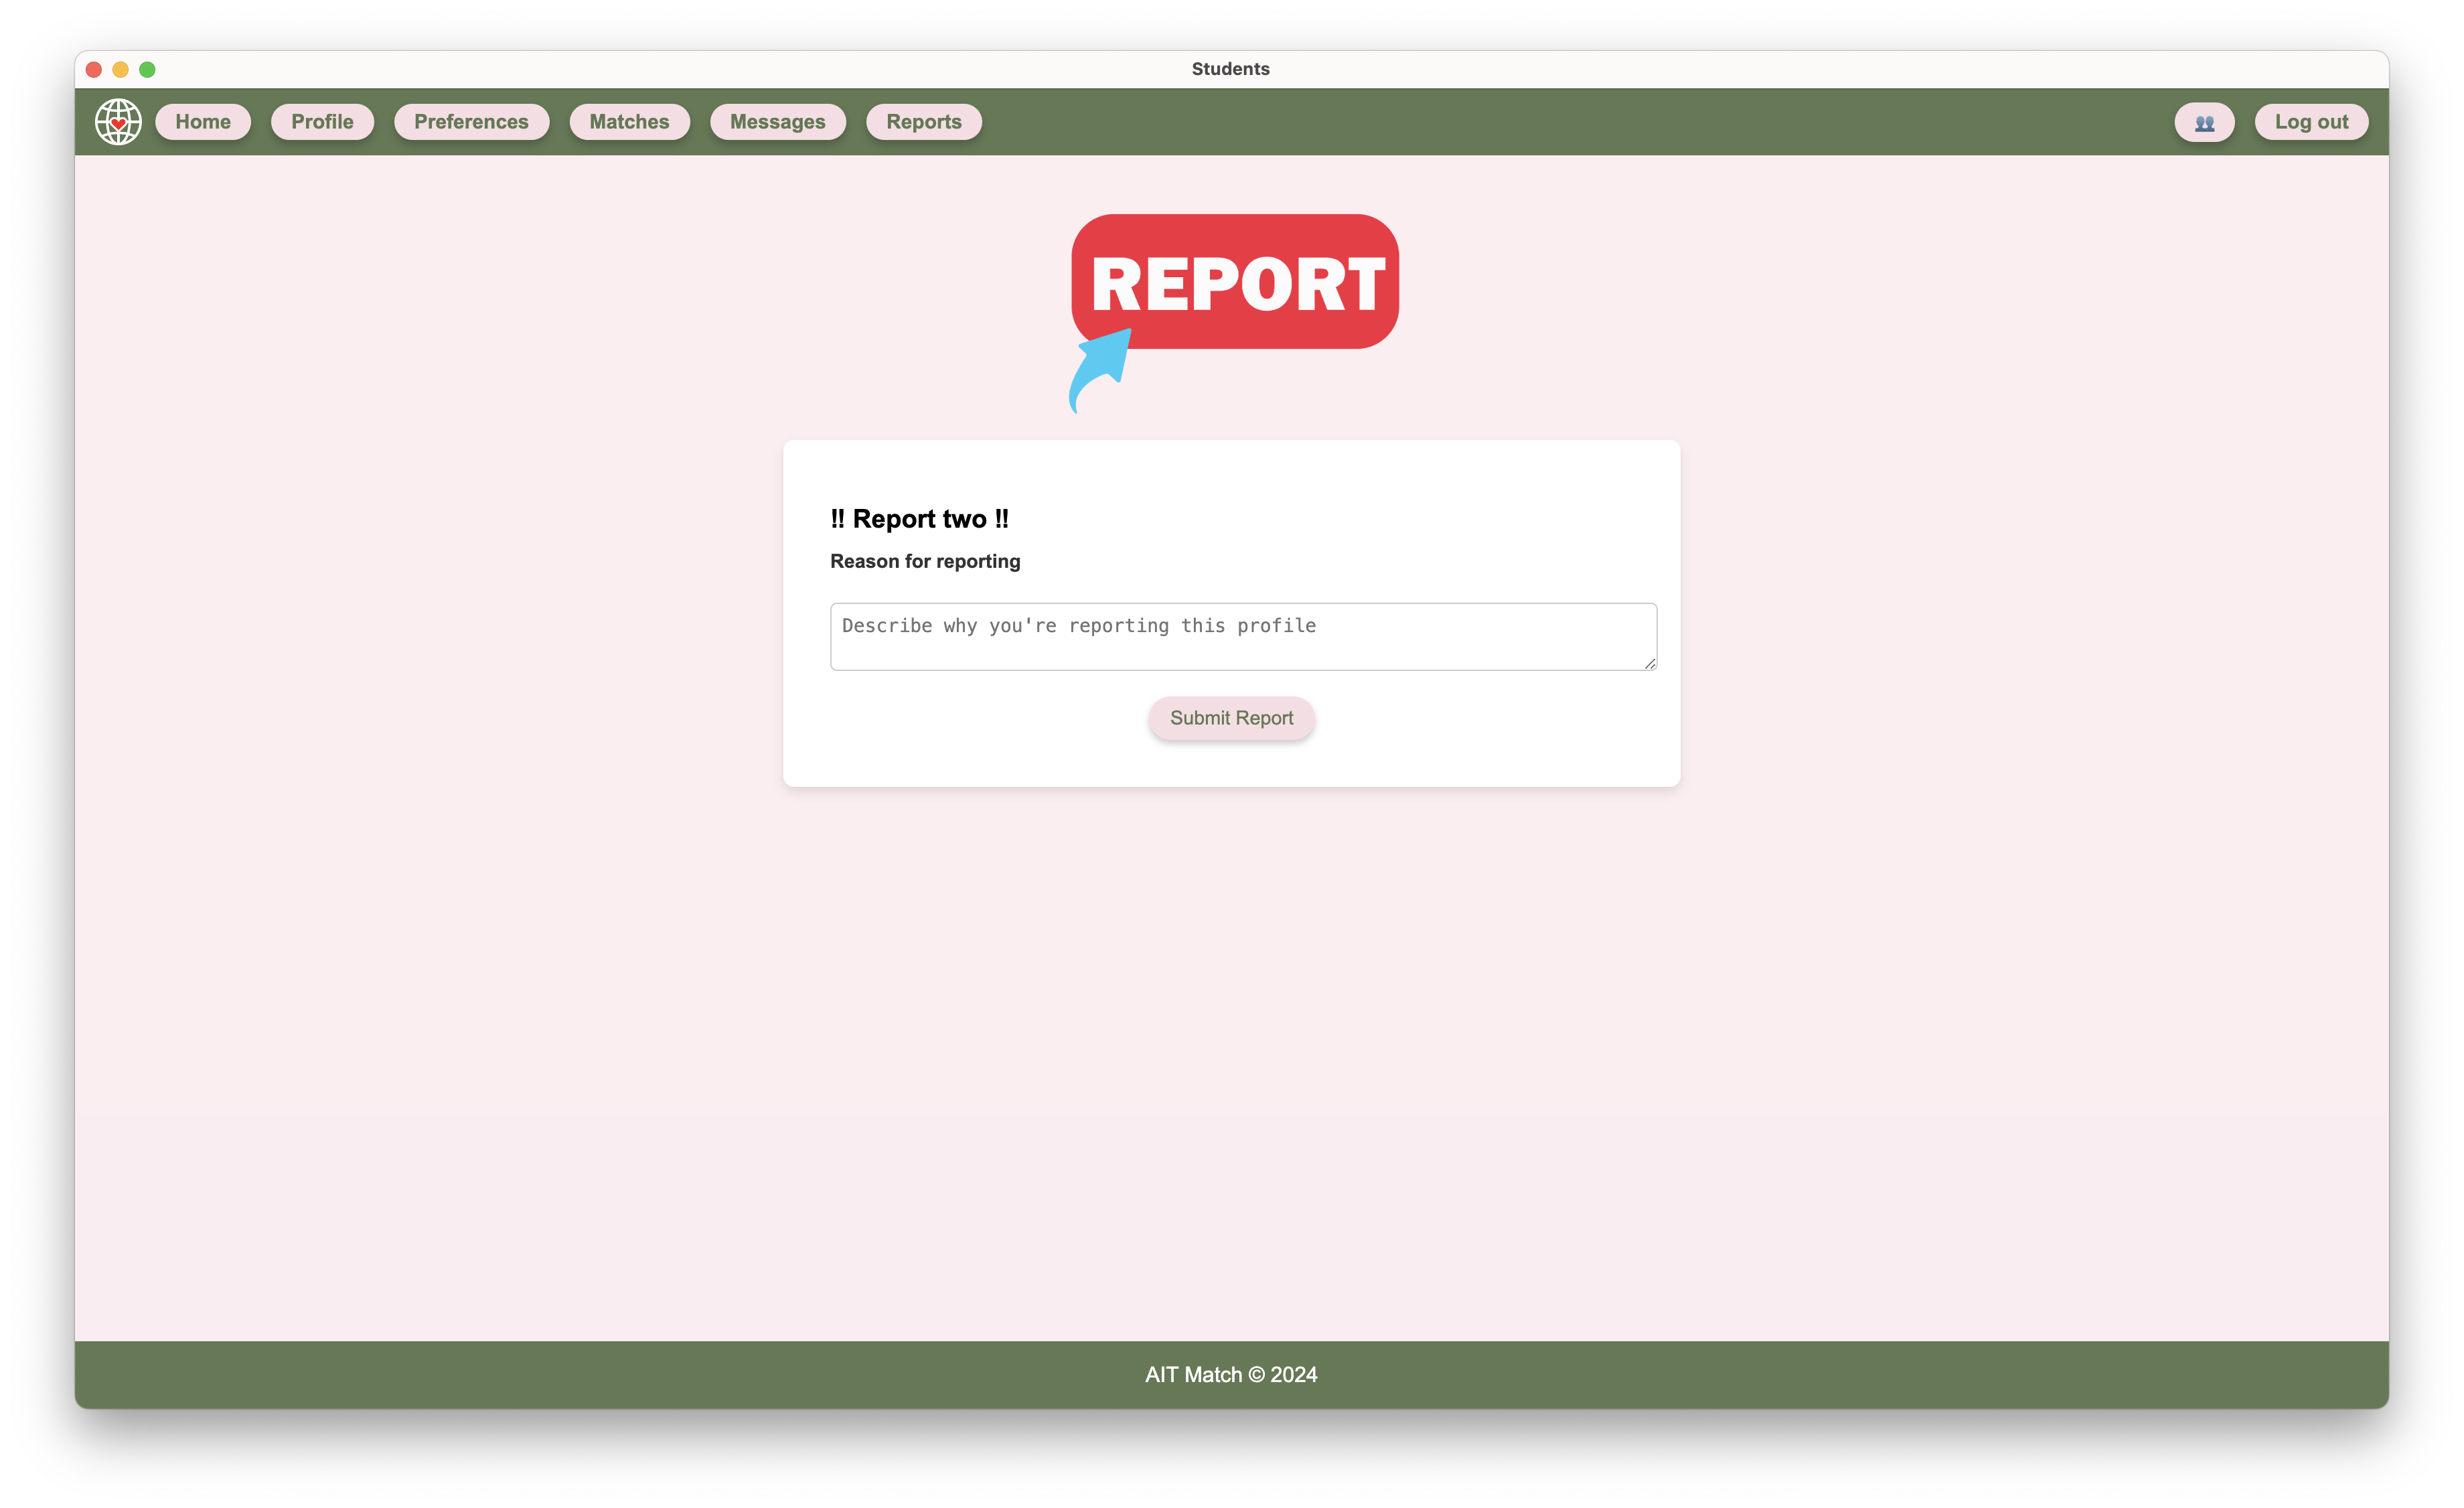
\includegraphics[width=5in]{figures/results/reports/report-new-page.png}
                \caption{New Report Page.}
                \label{fig:report-new-page}
            \end{figure}

        \newpage
        \subsection{Report: No Report Page}
        \begin{figure}[h]
                \centering
                \captionsetup{justification=centering, singlelinecheck=false, labelsep=space}
                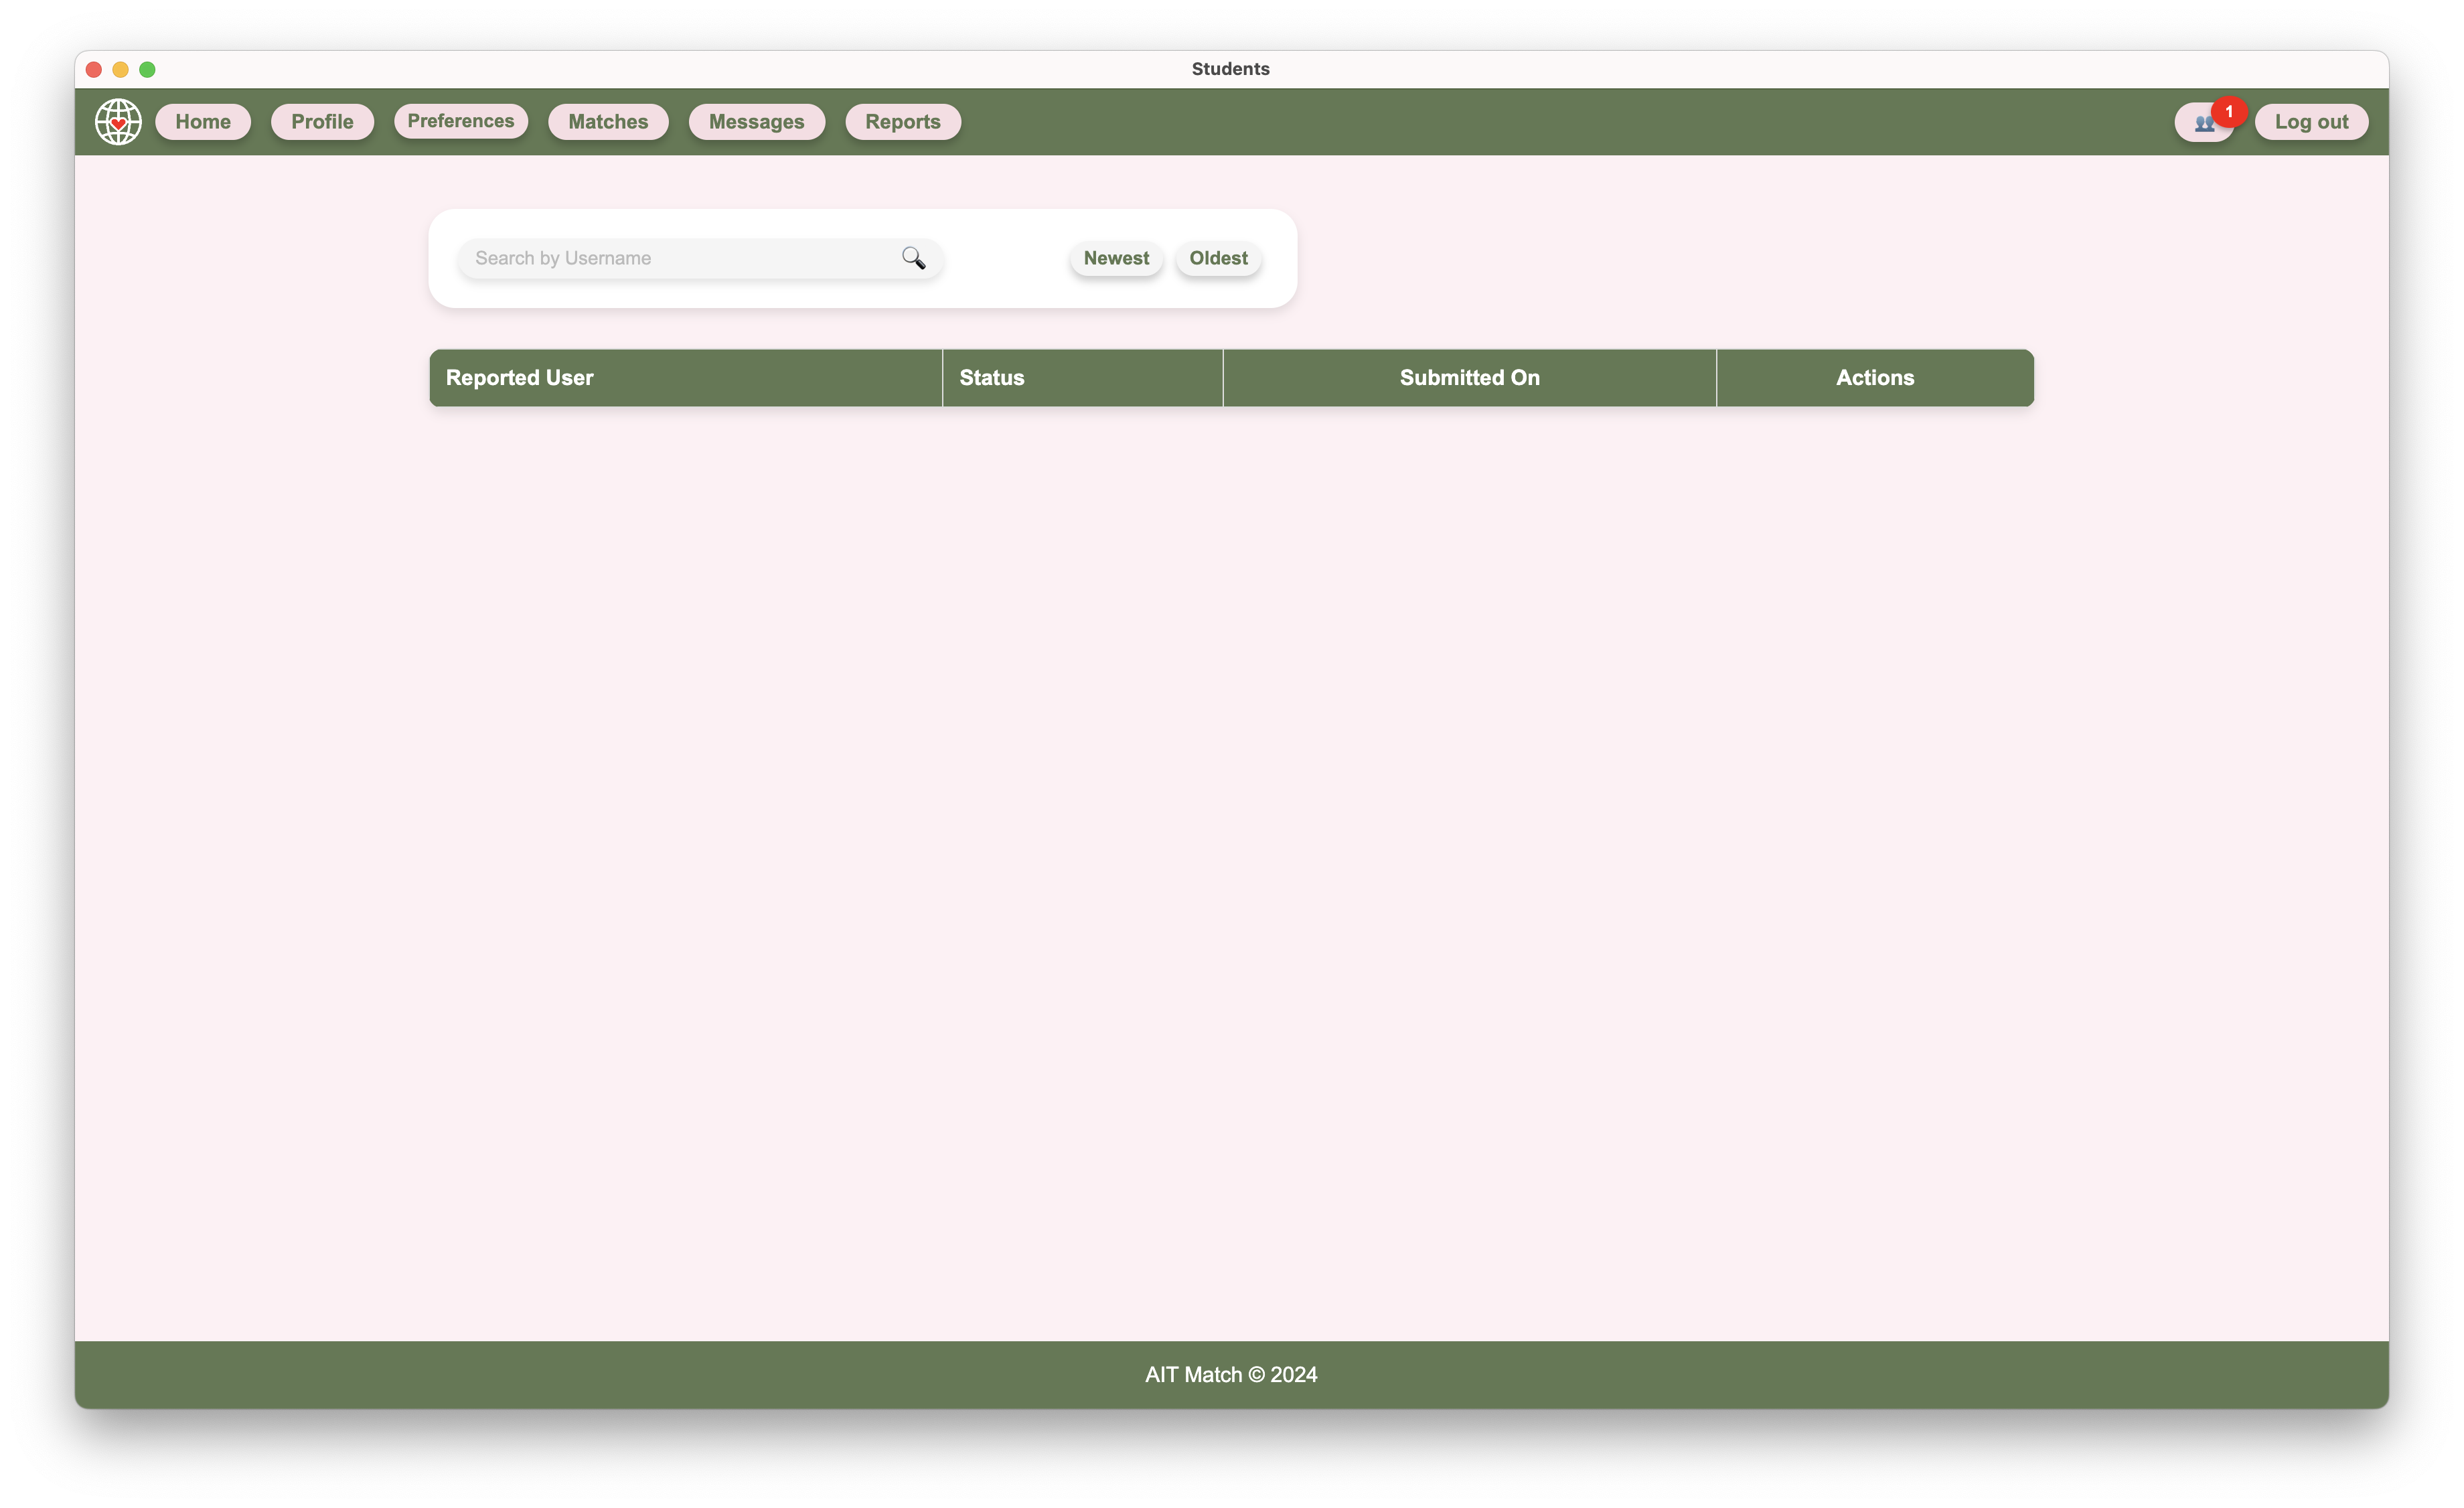
\includegraphics[width=5in]{figures/results/reports/no-reports-page.png}
                \caption{No Report Page.}
                \label{fig:no-reports-page}
            \end{figure}

        \subsection{Report: Report Index Page}
        \begin{figure}[h]
                \centering
                \captionsetup{justification=centering, singlelinecheck=false, labelsep=space}
                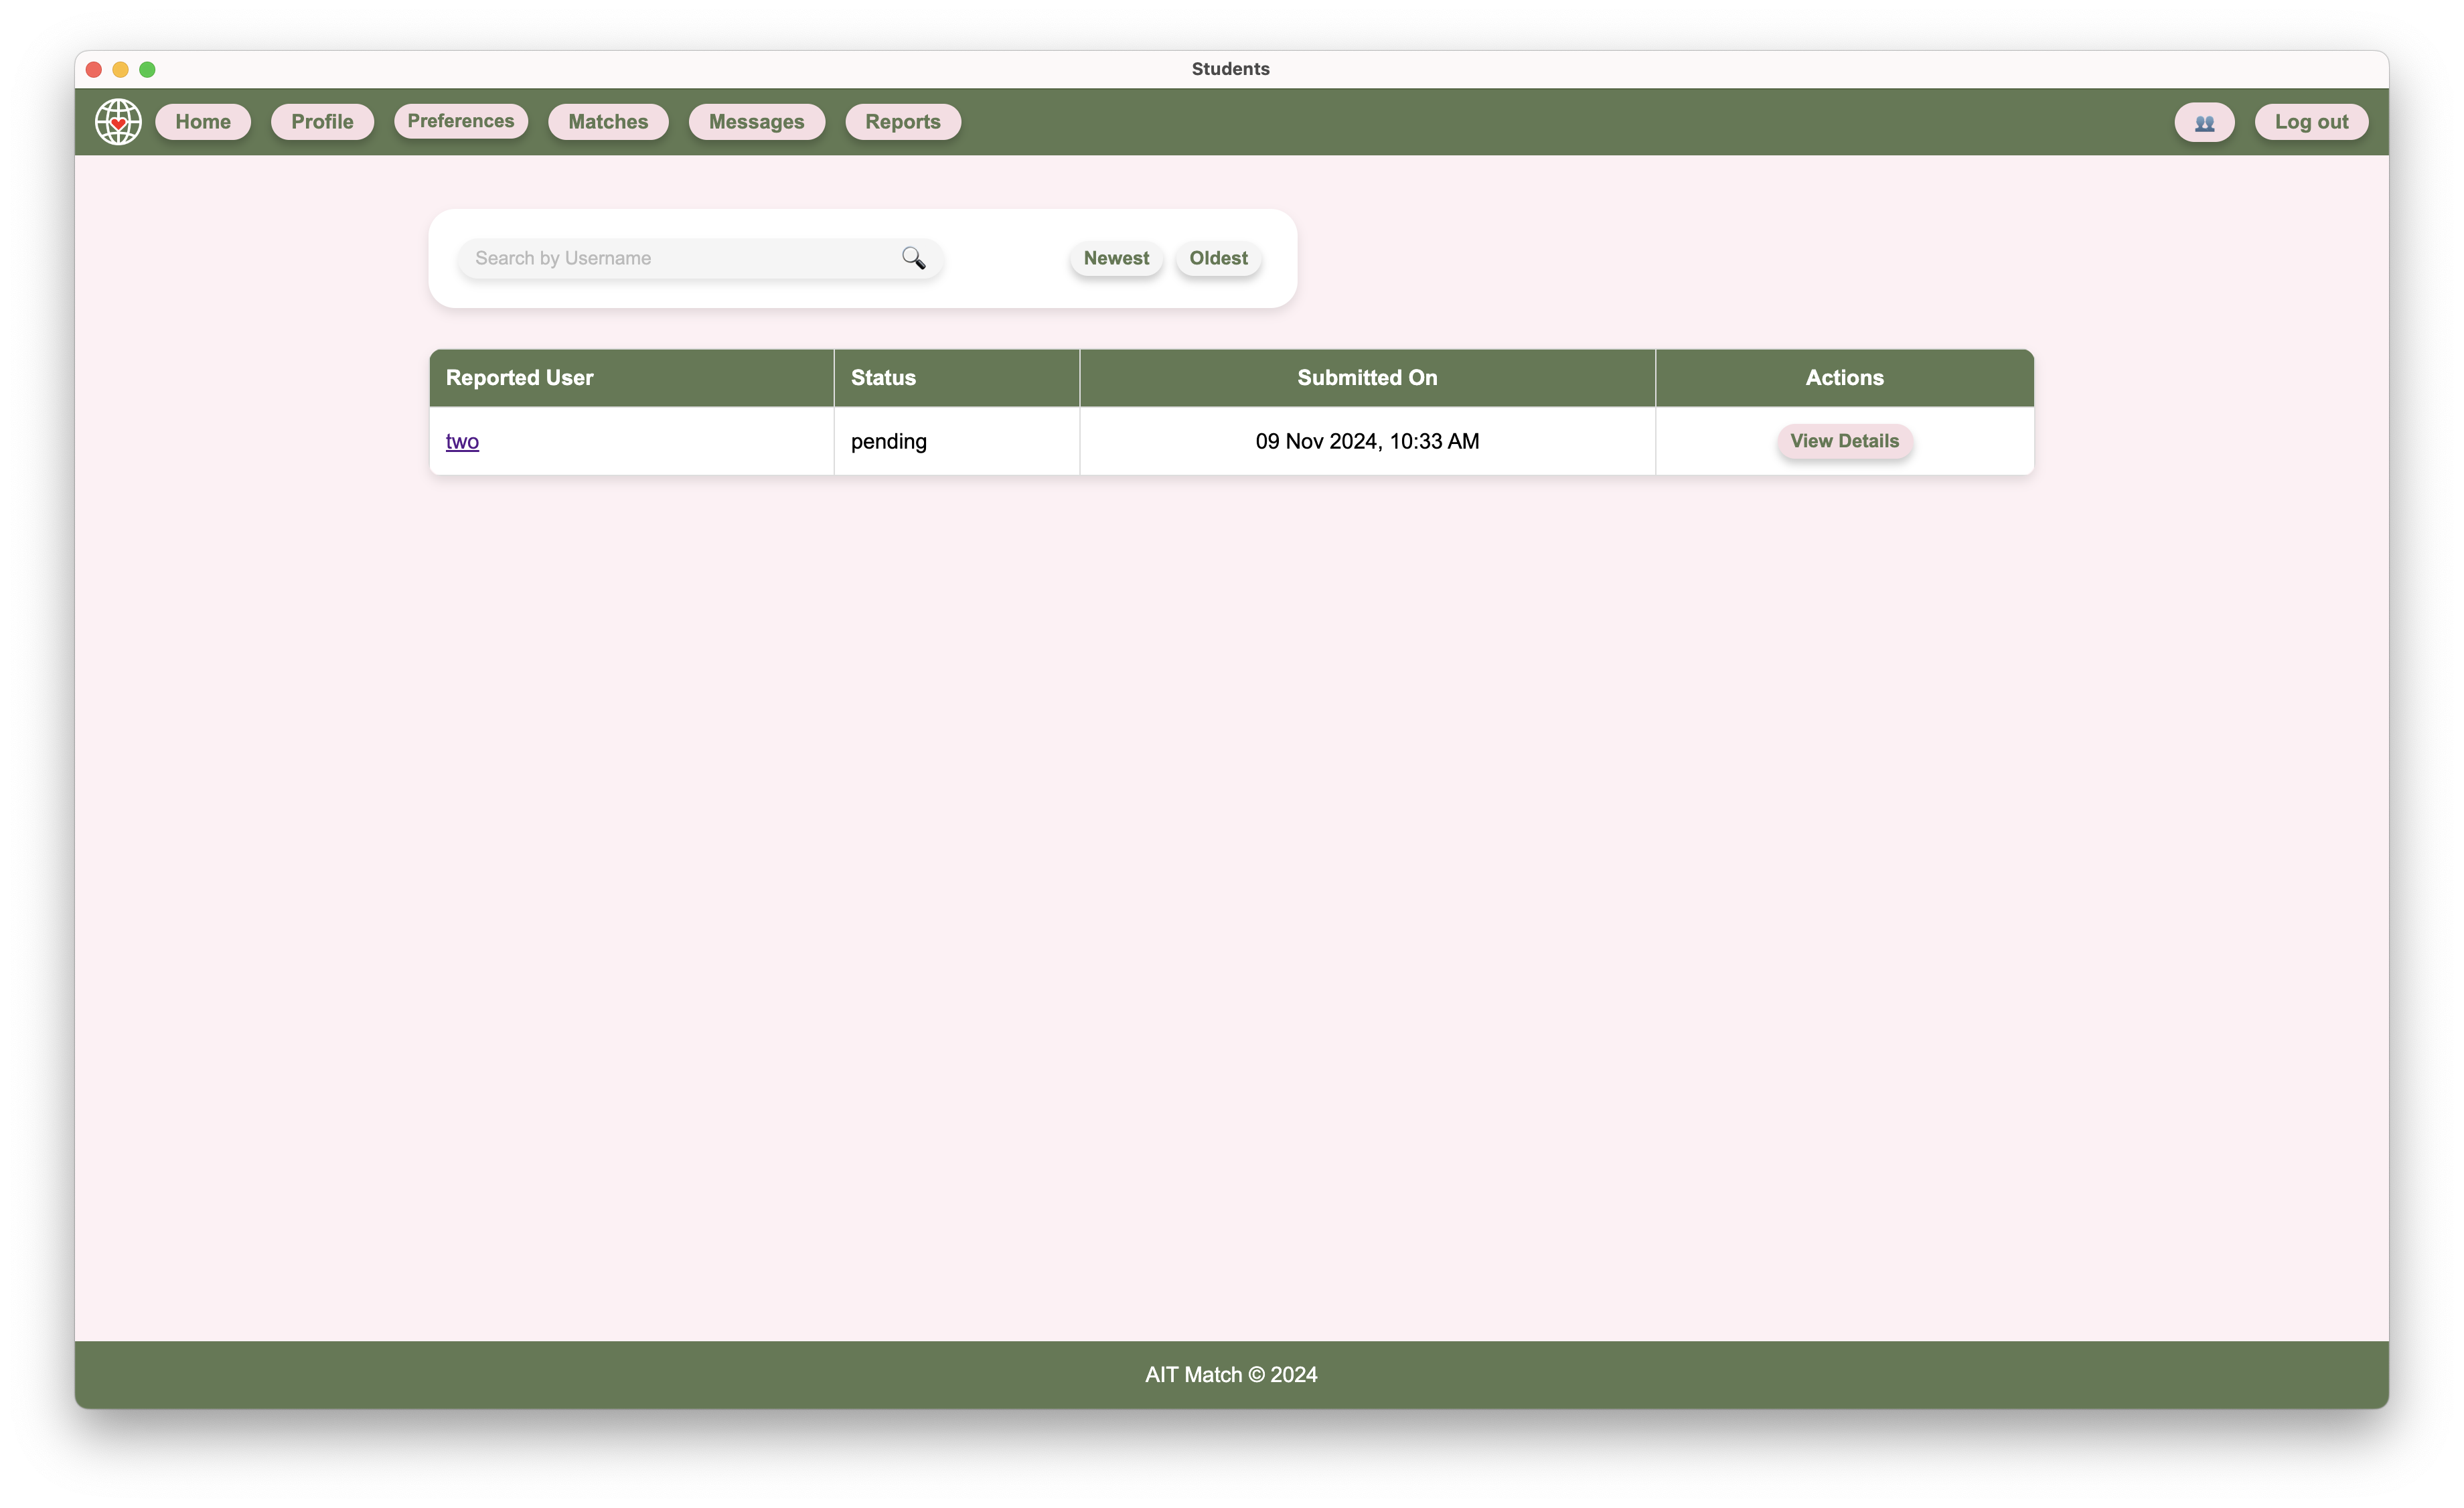
\includegraphics[width=5in]{figures/results/reports/report-index-page.png}
                \caption{Report Index Page.}
                \label{fig:report-index-page}
            \end{figure}

        \newpage
        \subsection{Report: Report Show Page}
        \begin{figure}[h]
                \centering
                \captionsetup{justification=centering, singlelinecheck=false, labelsep=space}
                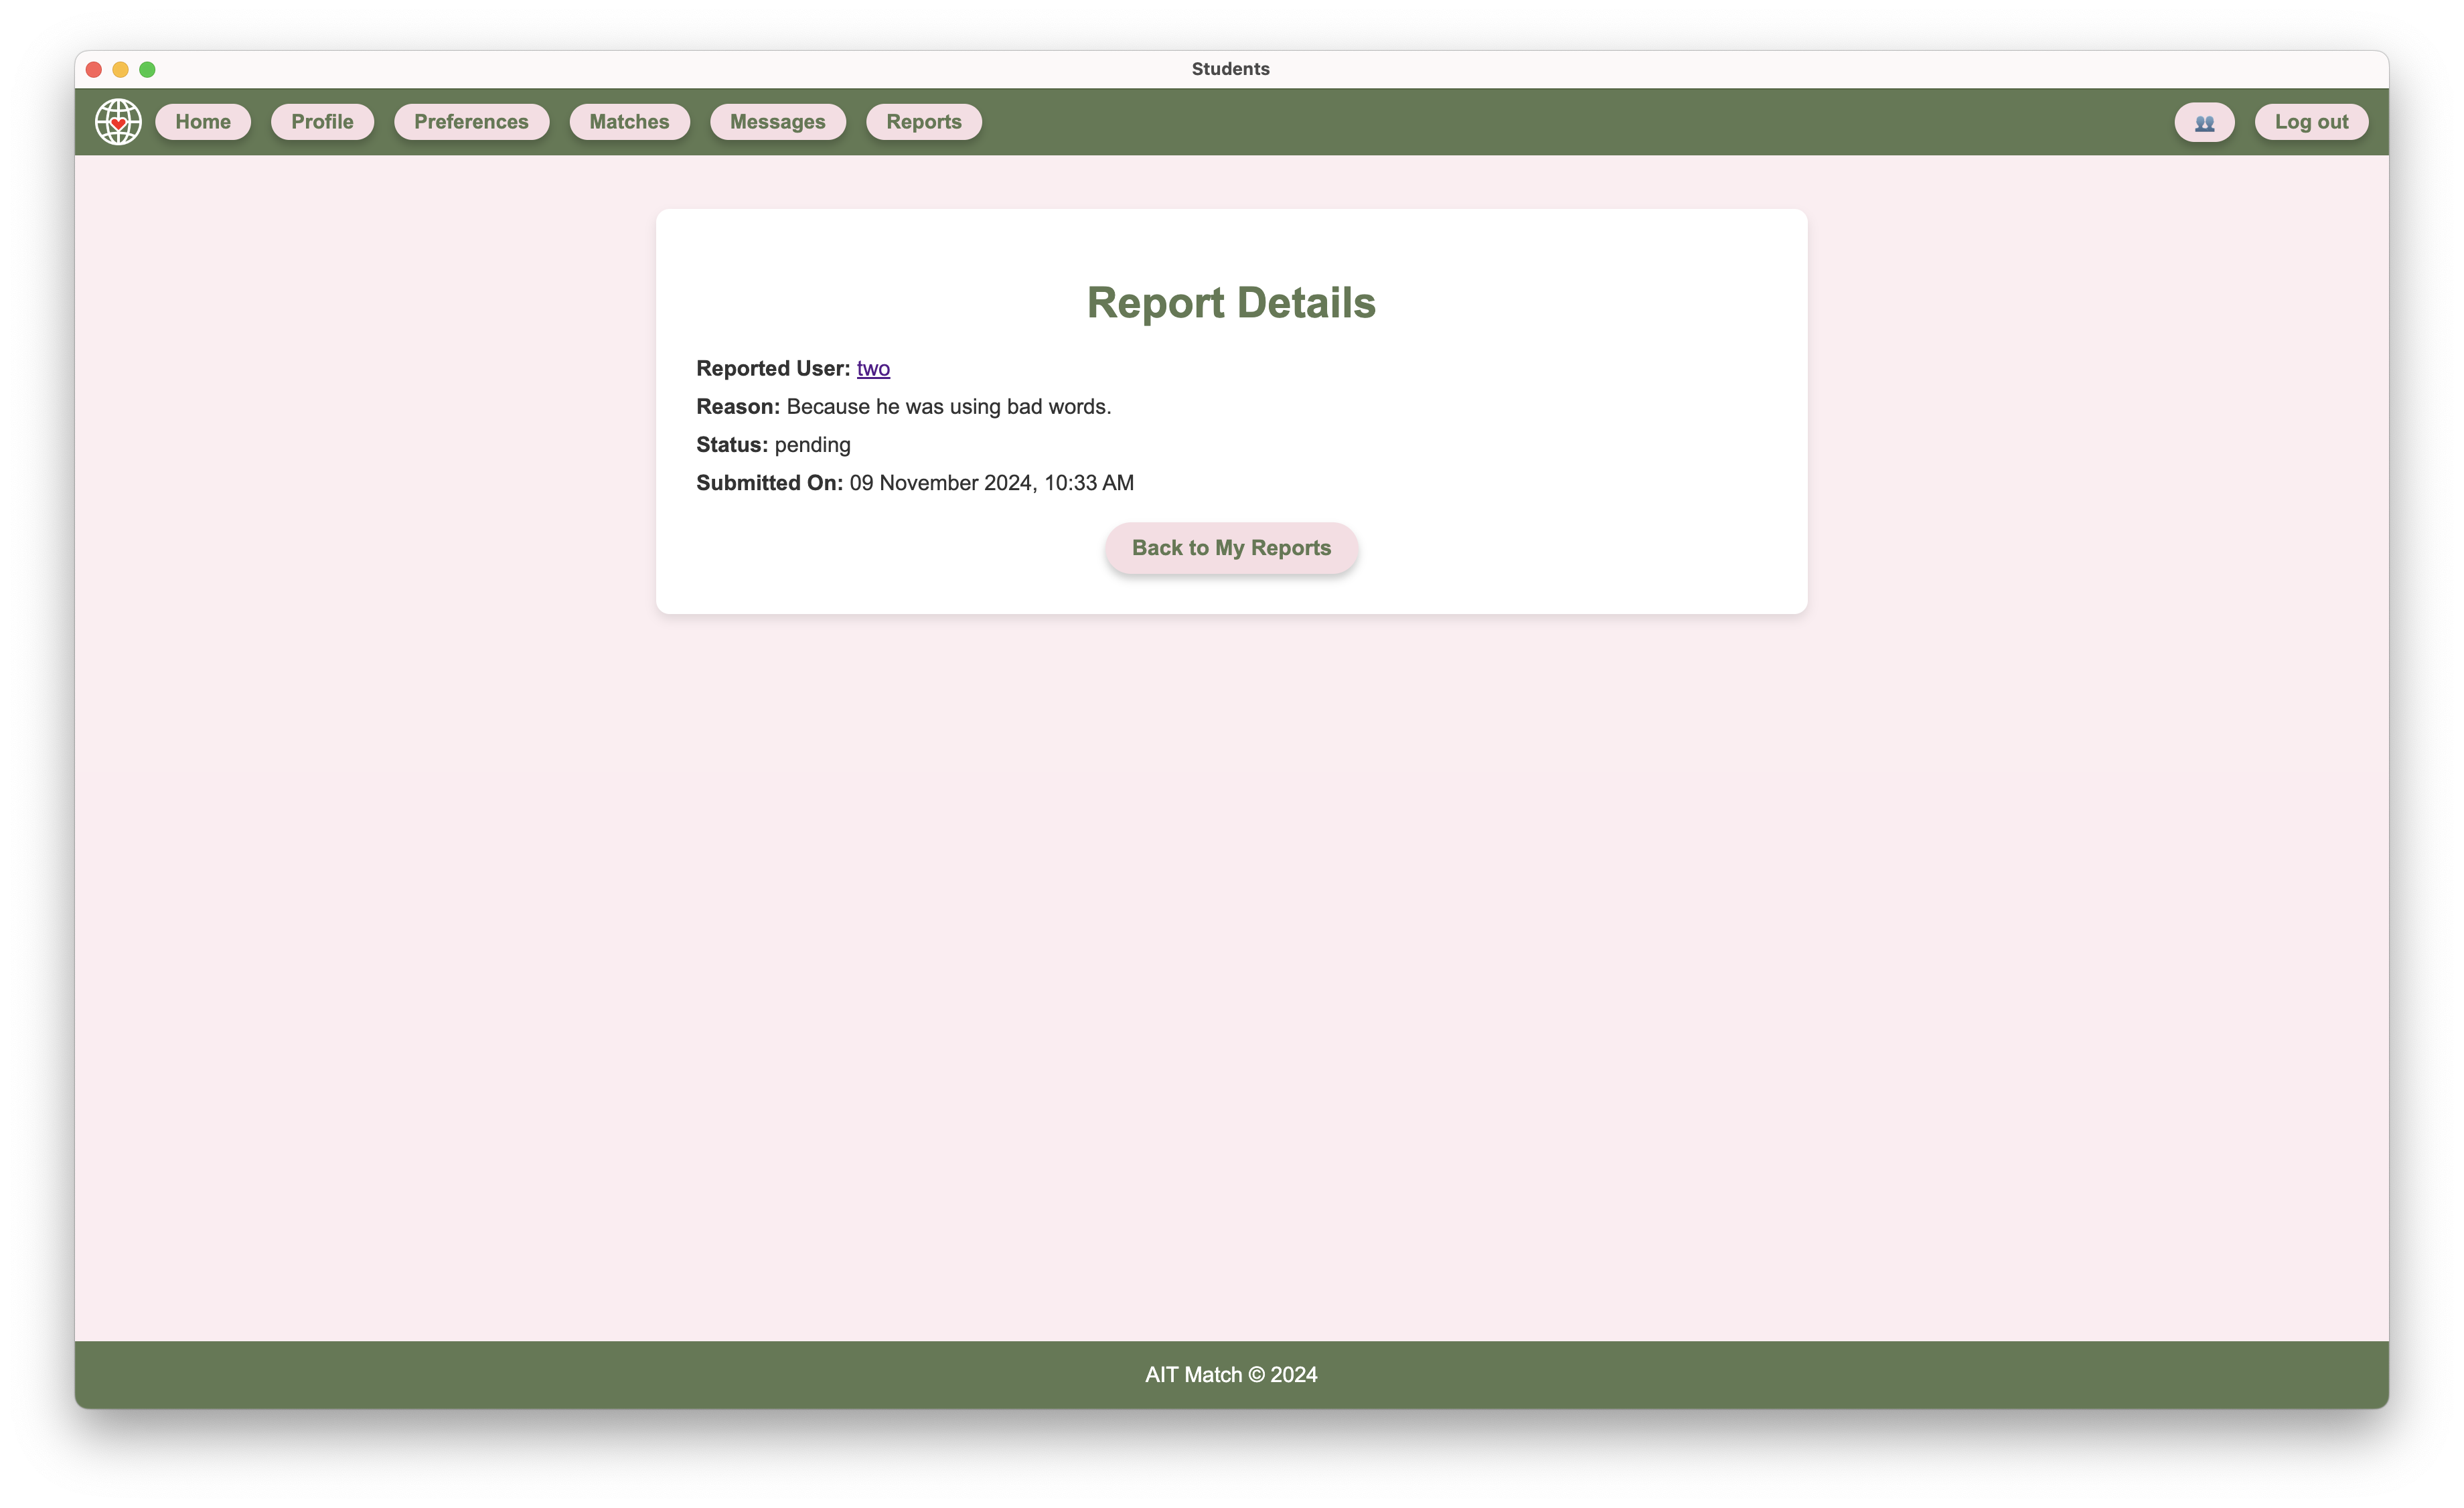
\includegraphics[width=5in]{figures/results/reports/report-show-page.png}
                \caption{Report Show Page.}
                \label{fig:report-show-page}
            \end{figure}
% ------------------------------------------------- %
        \newpage
        \subsection{Admin Panel: Users Management Page}
        \begin{figure}[h]
                \centering
                \captionsetup{justification=centering, singlelinecheck=false, labelsep=space}
                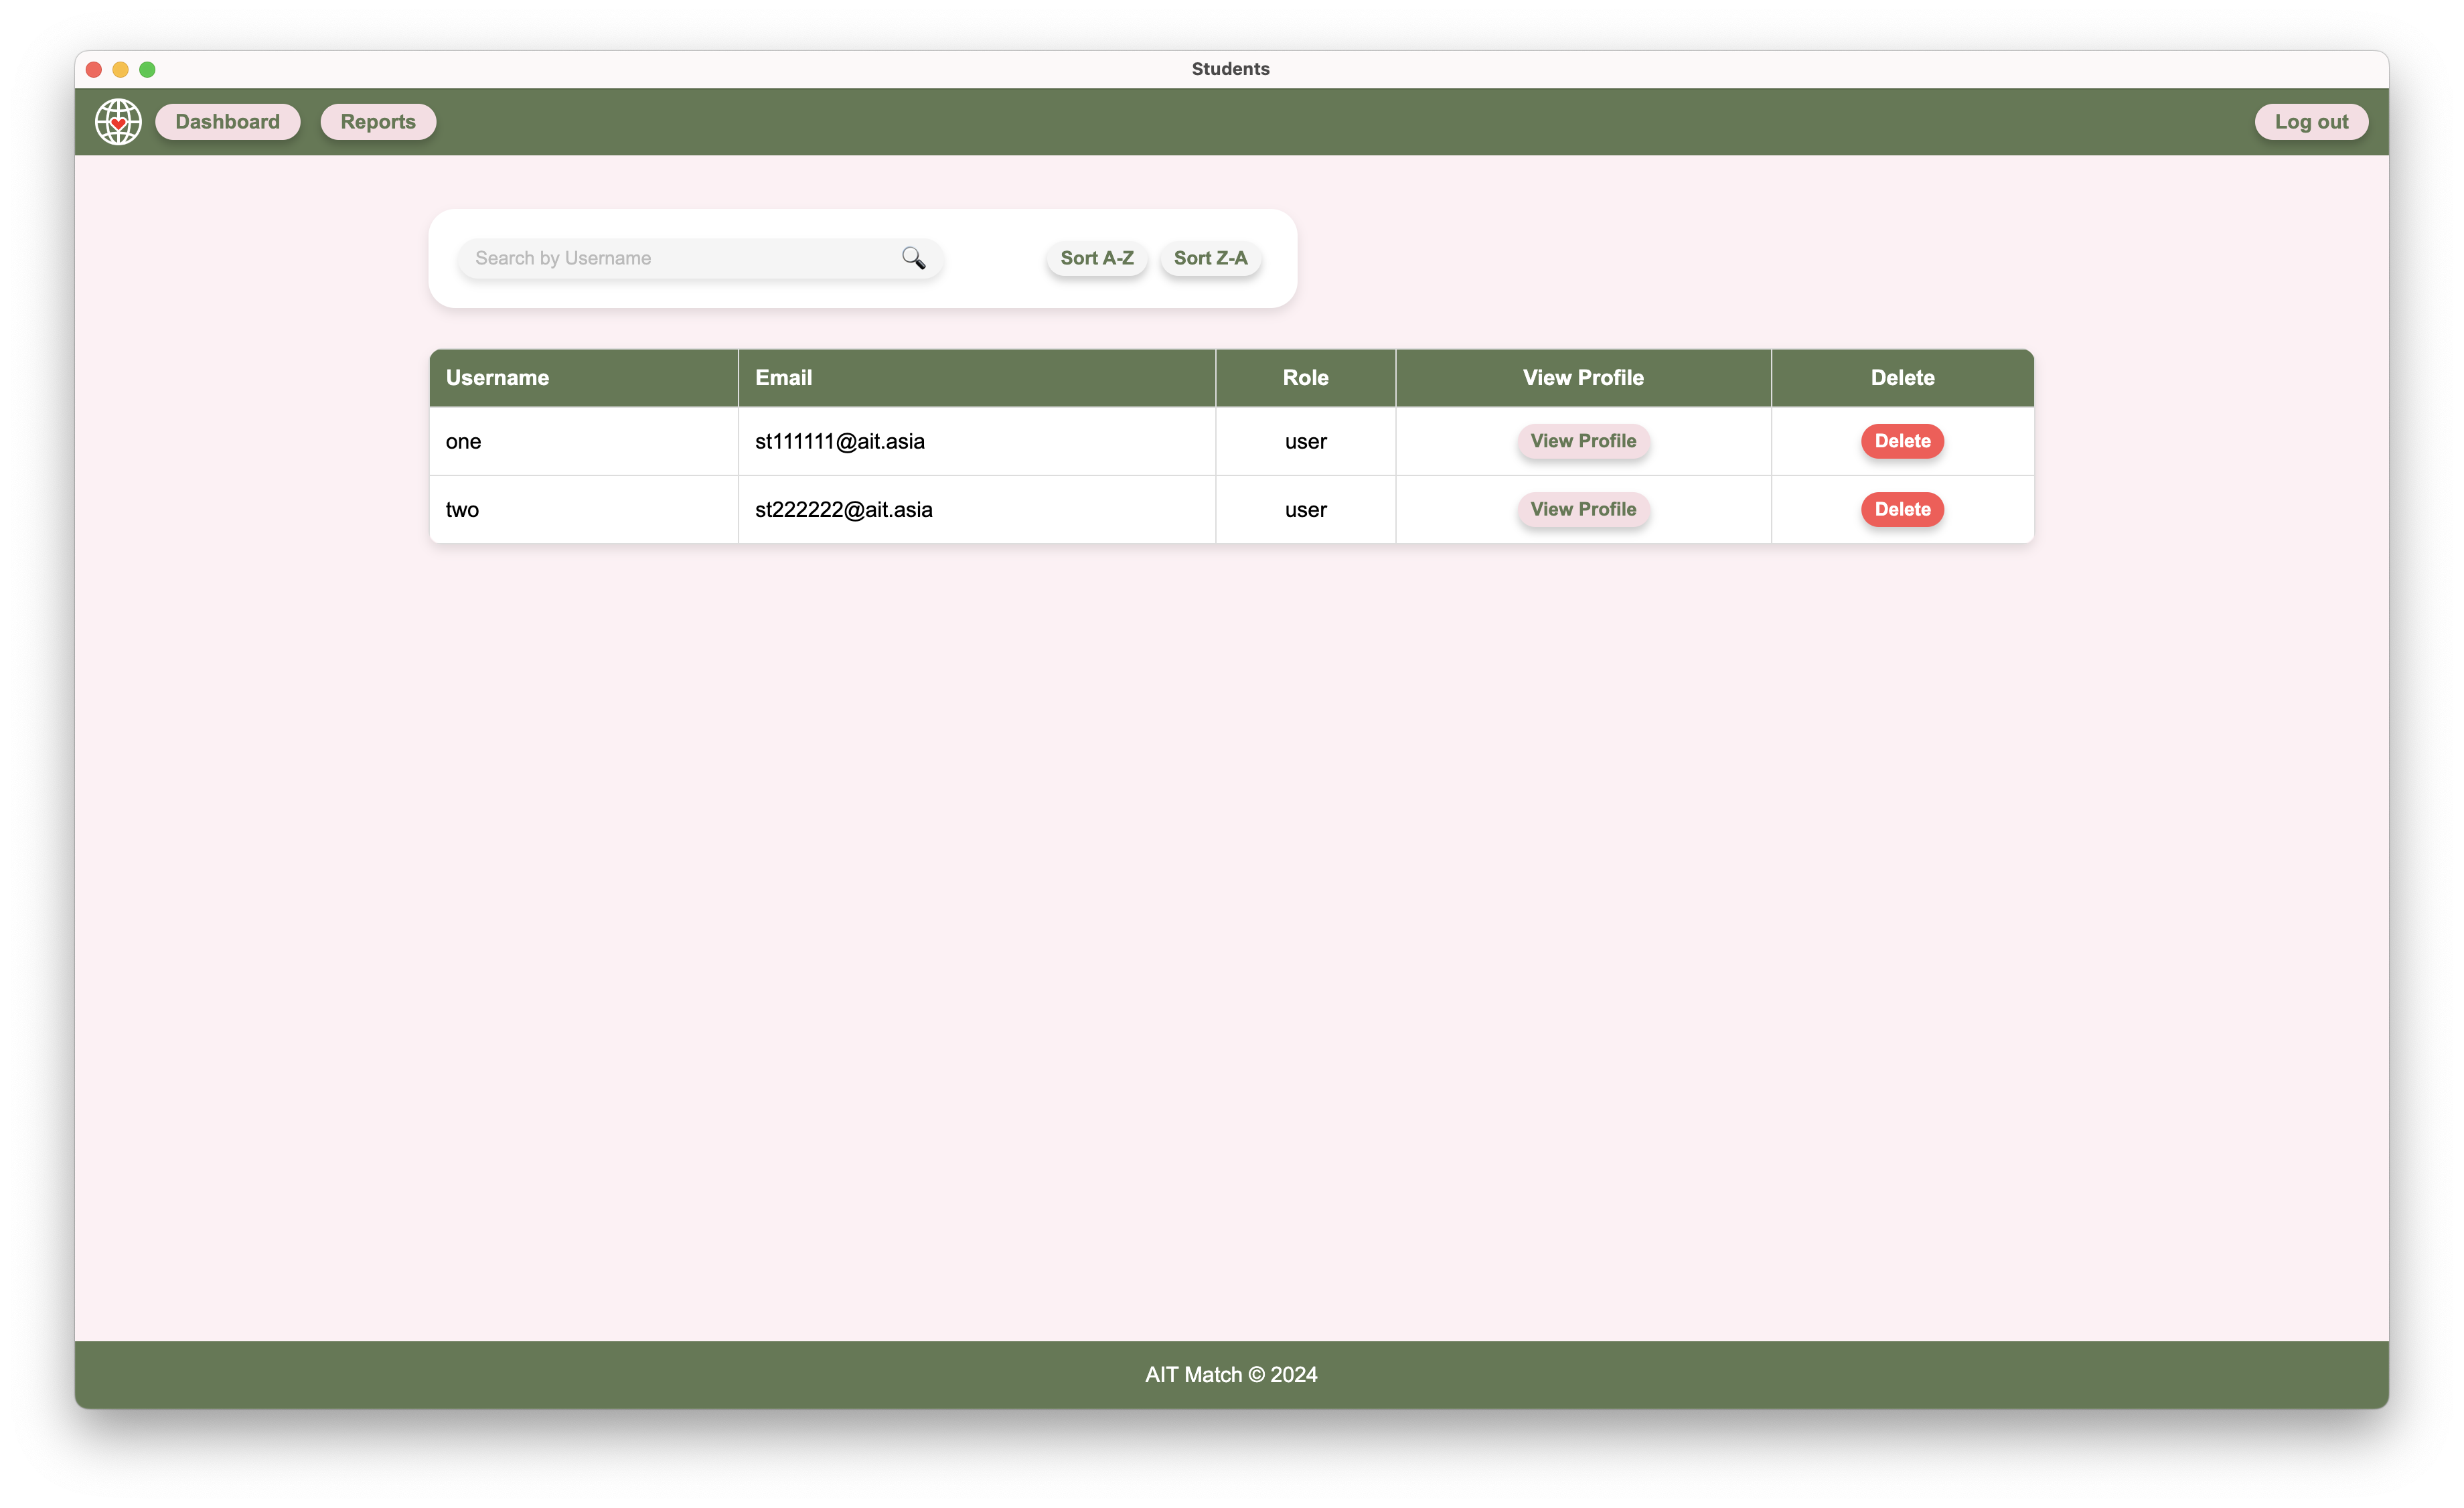
\includegraphics[width=5in]{figures/results/admin/user-management.png} 
                \caption{Admin Users Management Page.}
                \label{fig:user-management}
            \end{figure}

        \subsection{Admin Panel: Reports Management Page}
        \begin{figure}[h]
                \centering
                \captionsetup{justification=centering, singlelinecheck=false, labelsep=space}
                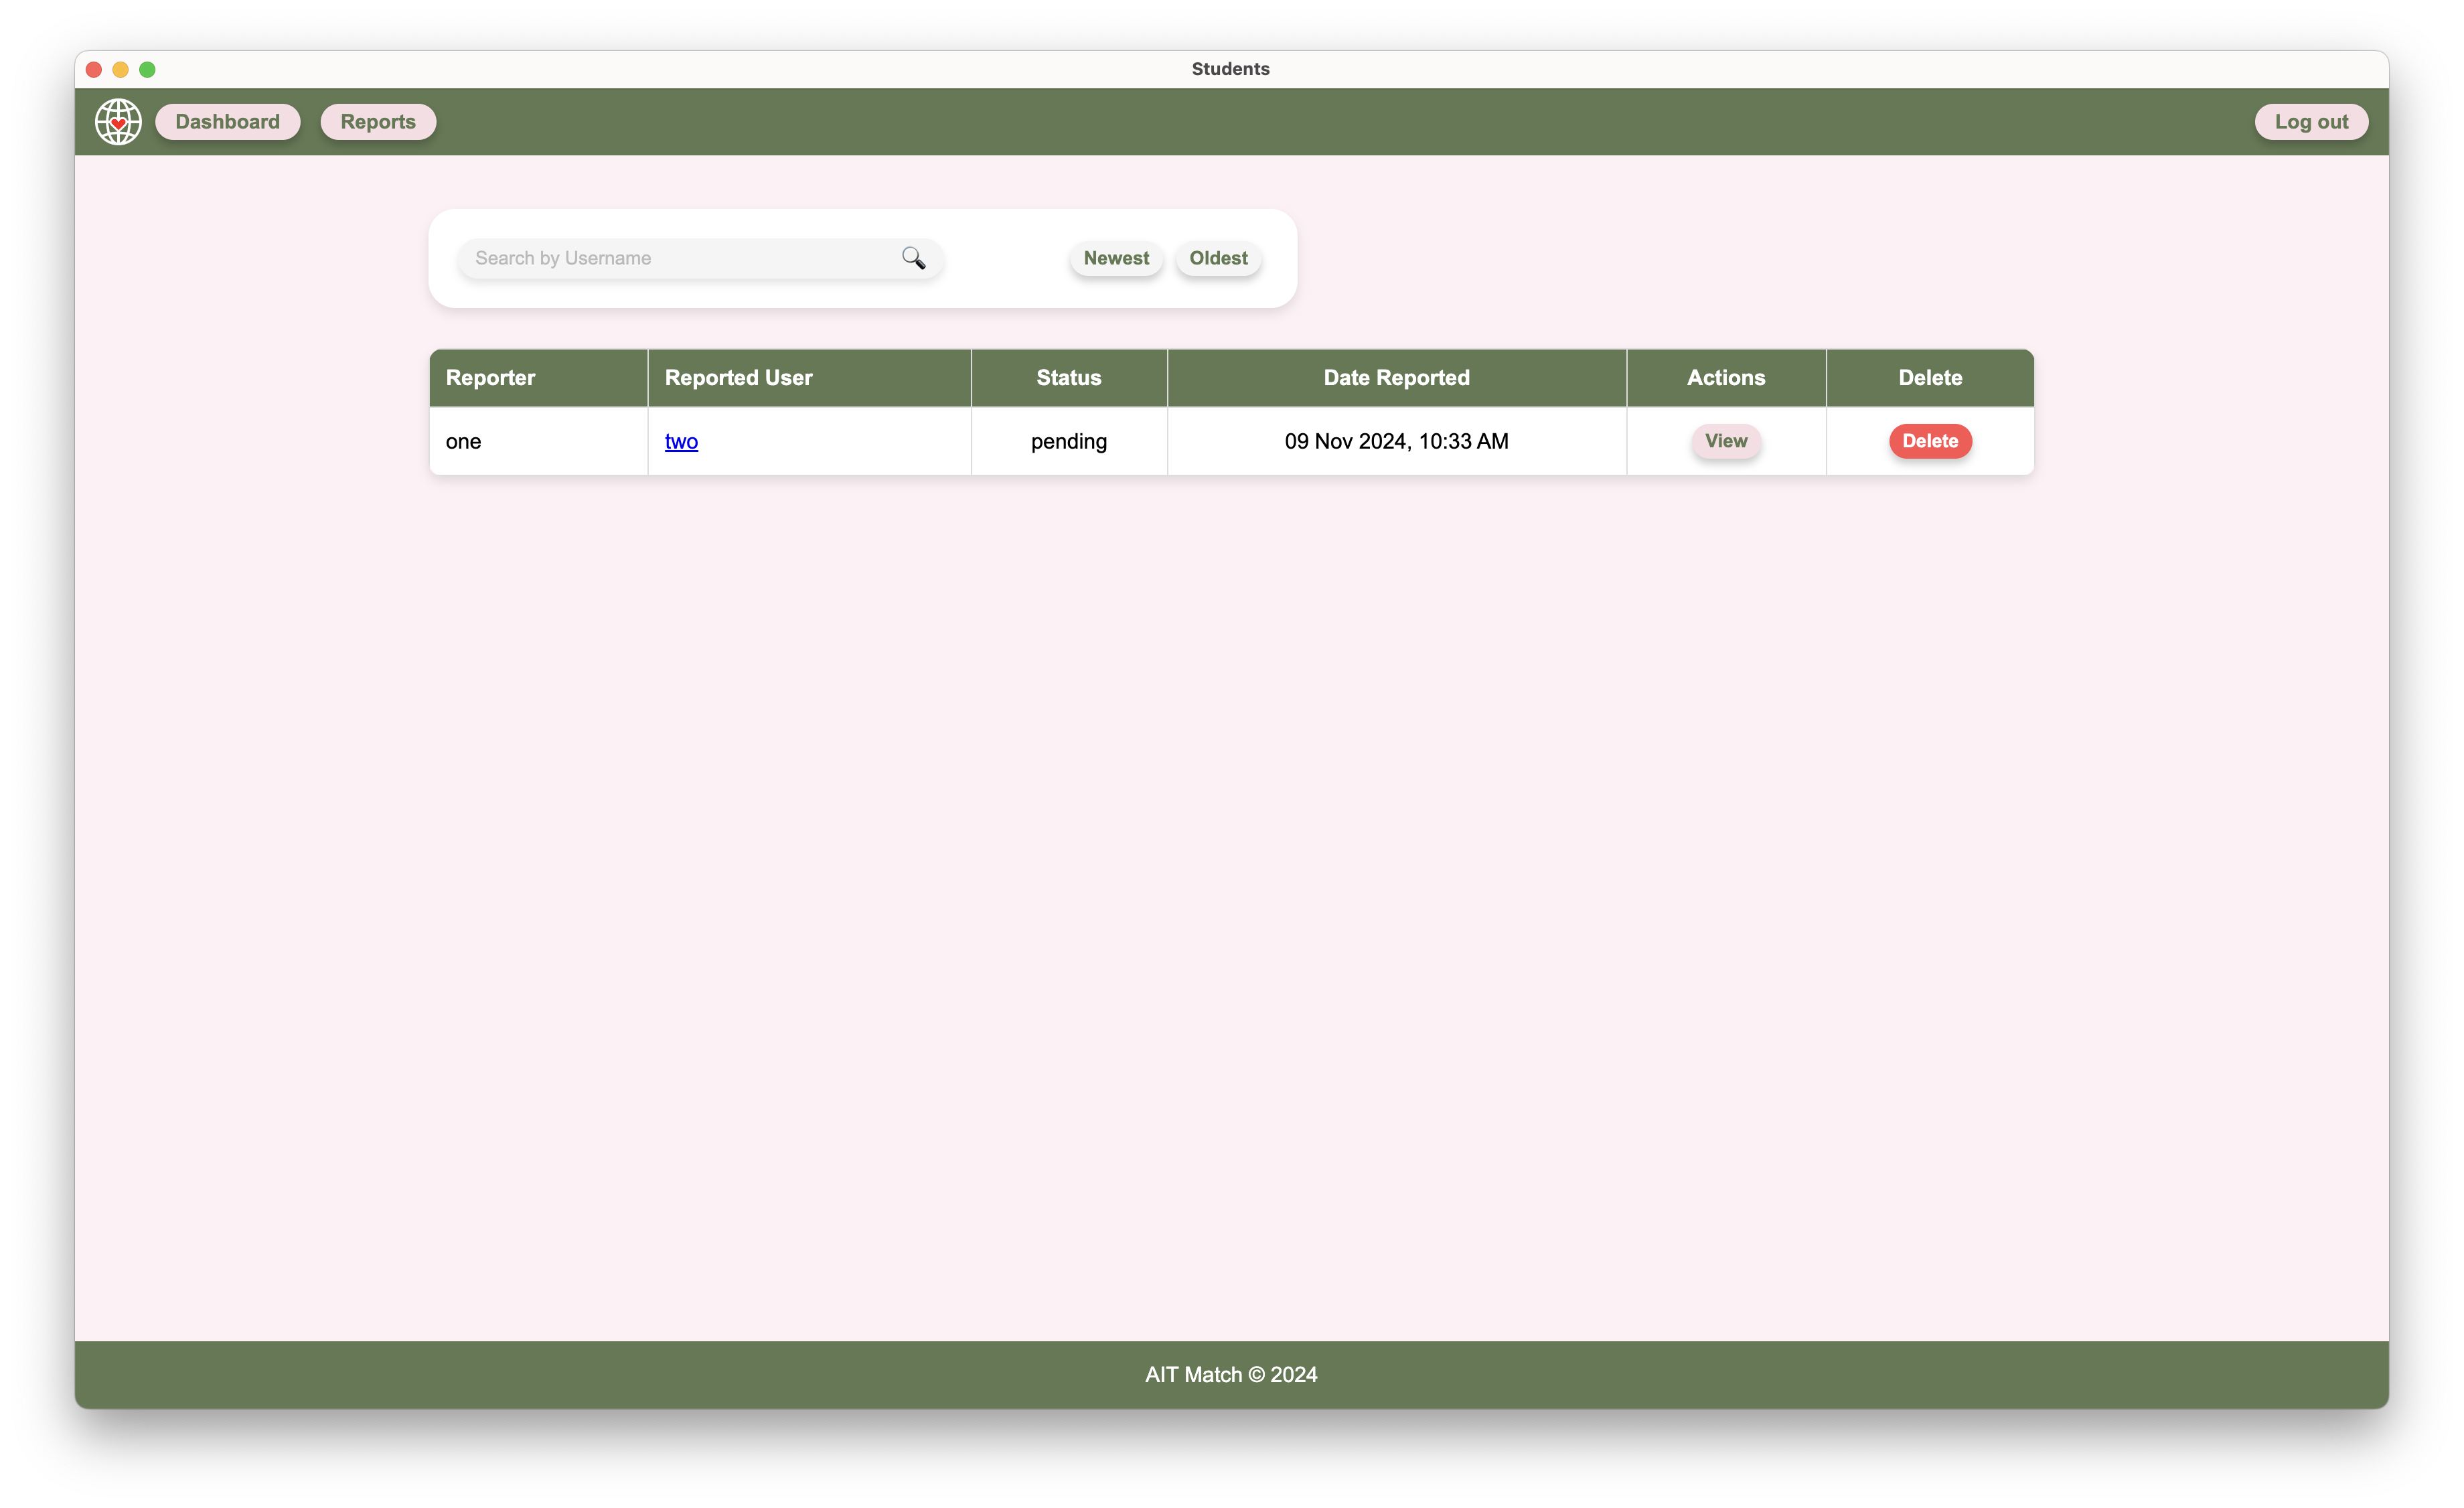
\includegraphics[width=5in]{figures/results/admin/report-management.png}
                \caption{Admin Reports Management Page.}
                \label{fig:report-management}
            \end{figure}

            


